%%%%%%%%%%%%%%%%%%%%%%%%%%%%%%%%%%%%%%%%%
% kaobook
% LaTeX Template
% Version 1.1 (23/6/19)
%
% This template originates from:
% https://www.LaTeXTemplates.com
%
% For the latest template development version and to make contributions:
% https://github.com/fmarotta/kaobook
%
% Authors:
% Federico Marotta (federicomarotta@mail.com)
% Based on the doctoral thesis of Ken Arroyo Ohori (https://3d.bk.tudelft.nl/ken/en)
% and on the Tufte-LaTeX class.
% Modified for LaTeX Templates by Vel (vel@latextemplates.com)
%
% License:
% CC0 1.0 Universal (see included MANIFEST.md file)
%
%%%%%%%%%%%%%%%%%%%%%%%%%%%%%%%%%%%%%%%%%

%----------------------------------------------------------------------------------------
%	PACKAGES AND OTHER DOCUMENT CONFIGURATIONS
%----------------------------------------------------------------------------------------

\documentclass[
	fontsize=10pt, % Base font size
	twoside=true, % Use different layouts for even and odd pages (in particular, if twoside=true, the margin column will be always on the outside)
	%open=any, % If twoside=true, uncomment this to force new chapters to start on any page, not only on right (odd) pages
	%chapterprefix=true, % Uncomment to use the word "Chapter" before chapter numbers everywhere they appear
	%chapterentrydots=true, % Uncomment to output dots from the chapter name to the page number in the table of contents
	numbers=noenddot, % Comment to output dots after chapter numbers; the most common values for this option are: enddot, noenddot and auto (see the KOMAScript documentation for an in-depth explanation)
	%draft=true, % If uncommented, rulers will be added in the header and footer
	%overfullrule=true, % If uncommented, overly long lines will be marked by a black box; useful for correcting spacing problems
]{kaobook}

% Load common packages and commands
\usepackage{styles/environments}
\usepackage{aas_macros}

% Load mathematical packages for theorems and related environments. NOTE: choose only one between 'mdftheorems' and 'plaintheorems'.
\usepackage{styles/mdftheorems}
%\usepackage{styles/plaintheorems}
\usepackage{quotchap}
% Load packages for testing
\usepackage{blindtext}
%\usepackage{showframe} % Uncomment to show boxes around the text area, margin, header and footer
%\usepackage{showlabels} % Uncomment to output the content of \label commands to the document where they are used

\usepackage{hyperref}
\usepackage{xcolor}
\hypersetup{
	colorlinks   = true, %Colours links instead of ugly boxes
}

\newcommand{\ztf}{\href{https://github.com/robertdstein/AMPEL_followup_pipeline/releases/tag/v1.0.0}{\emph{AMPEL Follow-up Pipeline}}}
\newcommand{\Msol}{\mbox{$M_{\odot}$}}
\newcommand{\arcdeg}{\mbox{$^\circ$}}
\newcommand{\arcsec}{$^{\prime\prime}$}
\newcommand{\arcmin}{$^{\prime}$}

\graphicspath{{images/}{./}{figures/}} % Paths in which to look for images

\addbibresource{main.bib} % Bibliography file

\makeindex[columns=3, title=Alphabetical Index, intoc] % Make LaTeX produce the files required to compile the index

\makeglossaries % Make LaTeX produce the files required to compile the glossary

\makenomenclature % Make LaTeX produce the files required to compile the nomenclature

\usepackage{lipsum}
%%%%********************************************************************
% fancy quotes
\definecolor{quotemark}{gray}{0.7}
\makeatletter
\def\fquote{%
	\@ifnextchar[{\fquote@i}{\fquote@i[]}%]
}%
\def\fquote@i[#1]{%
	\def\tempa{#1}%
	\@ifnextchar[{\fquote@ii}{\fquote@ii[]}%]
}%
\def\fquote@ii[#1]{%
	\def\tempb{#1}%
	\@ifnextchar[{\fquote@iii}{\fquote@iii[]}%]
}%
\def\fquote@iii[#1]{%
	\def\tempc{#1}%
	\vspace{1em}%
	\noindent%
	\begin{list}{}{%
			\setlength{\leftmargin}{0.1\textwidth}%
			\setlength{\rightmargin}{0.1\textwidth}%
		}%
		\item[]%
		\begin{picture}(0,0)%
		\put(-15,-5){\makebox(0,0){\scalebox{3}{\textcolor{quotemark}{``}}}}%
		\end{picture}%
		\begingroup\itshape}%
	%%%%********************************************************************
	\def\endfquote{%
		\endgroup\par%
		\makebox[0pt][l]{%
			\hspace{0.8\textwidth}%
			\begin{picture}(0,0)(0,0)%
			\put(15,15){\makebox(0,0){%
					\scalebox{3}{\color{quotemark}''}}}%
			\end{picture}}%
		\ifx\tempa\empty%
		\else%
		\ifx\tempc\empty%
		\hfill\rule{100pt}{0.5pt}\\\mbox{}\hfill\tempa,\ \emph{\tempb}%
		\else%
		\hfill\rule{100pt}{0.5pt}\\\mbox{}\hfill\tempa,\ \emph{\tempb},\ \tempc%
		\fi\fi\par%
		\vspace{0.5em}%
	\end{list}%
}%
\makeatother

%----------------------------------------------------------------------------------------

\begin{document}

%----------------------------------------------------------------------------------------
%	BOOK INFORMATION
%----------------------------------------------------------------------------------------


%\subject{Use this document as a template}

\title[Multi-Messenger Observations of the Dynamic Universe]{Multi-Messenger Observations of the Dynamic Universe
\subtitle{Searching for sources of astrophysical neutrinos and gravitational waves}

\author[Robert Stein]{Robert Stein}}

\date{\today}

\publishers{An Awesome Publisher}

%----------------------------------------------------------------------------------------

\frontmatter % Denotes the start of the pre-document content, uses roman numerals

%----------------------------------------------------------------------------------------
%	OPENING PAGE
%----------------------------------------------------------------------------------------

%\makeatletter
%\extratitle{
%	% In the title page, the title is vspaced by 9.5\baselineskip
%	\vspace*{9\baselineskip}
%	\vspace*{\parskip}
%	\begin{center}
%		% In the title page, \huge is set after the komafont for title
%		\usekomafont{title}\huge\@title
%	\end{center}
%}
%\makeatother

%----------------------------------------------------------------------------------------
%	COPYRIGHT PAGE
%----------------------------------------------------------------------------------------

\makeatletter
\uppertitleback{\@titlehead} % Header

\lowertitleback{
	\textbf{Disclaimer}\\
	You can edit this page to suit your needs. For instance, here we have a no copyright statement, a colophon and some other information. This page is based on the corresponding page of Ken Arroyo Ohori's thesis, with minimal changes.
	
	\medskip
	
	\textbf{No copyright}\\
	\cczero\ This book is released into the public domain using the CC0 code. To the extent possible under law, I waive all copyright and related or neighbouring rights to this work.
	
	To view a copy of the CC0 code, visit: \\\url{http://creativecommons.org/publicdomain/zero/1.0/}
	
	\medskip
	
	\textbf{Colophon} \\
	This document was typeset with the help of \href{https://sourceforge.net/projects/koma-script/}{\KOMAScript} and \href{ttps://www.latex-project.org/}{\LaTeX} using the \href{https://github.com/fmarotta/kaobook/}{kaobook} class.
	
	The source code of this book is available at:\\\url{https://github.com/fmarotta/kaobook}
	
	THE CODE UseD TO PRODUCE PLOTS IN THis thesis can be found at...
		
	(You are welcome to contribute!)
	
	\medskip
	
	\textbf{Publisher} \\
	First printed in May 2019 by \@publishers
}
\makeatother

%----------------------------------------------------------------------------------------
%	DEDICATION
%----------------------------------------------------------------------------------------

\dedication{
	A neutrino is not a big thing to be hit by. \\
	
	In fact it's hard to think of anything much smaller by which one could reasonably hope to be hit. And it's not as if being hit by neutrinos was in itself a particularly unusual event for something the size of the Earth. Far from it. It would be an unusual nanosecond in which the Earth was not hit by several billion passing neutrinos.\\
	\flushright --\textit{The Hitchhiker's Guide to The Galaxy}

}

%----------------------------------------------------------------------------------------
%	OUTPUT TITLE PAGE AND PREVIOUS
%----------------------------------------------------------------------------------------

% Note that \maketitle outputs the pages before here

% If twoside=false, \uppertitleback and \lowertitleback are not printed
% To overcome this issue, we set twoside=semi just before printing the title pages, and set it back to false just after the title pages
\KOMAoptions{twoside=semi}
\maketitle
\KOMAoptions{twoside=false}

%----------------------------------------------------------------------------------------
%	PREFACE
%----------------------------------------------------------------------------------------

\chapter{Abstract}

Neutrinos are great, probably


%----------------------------------------------------------------------------------------
%	TABLE OF CONTENTS & LIST OF FIGURES/TABLES
%----------------------------------------------------------------------------------------

\begingroup % Local scope for the following commands

% Define the style for the TOC, LOF, and LOT
%\setstretch{1} % Uncomment to modify line spacing in the ToC
%\hypersetup{linkcolor=blue} % Uncomment to set the colour of links in the ToC
\setlength{\textheight}{23cm} % Manually adjust the height of the ToC pages

% Turn on compatibility mode for the etoc package
\etocstandarddisplaystyle % "toc display" as if etoc was not loaded
\etocstandardlines % "toc lines as if etoc was not loaded

\tableofcontents % Output the table of contents

\listoffigures % Output the list of figures

% Comment both of the following lines to have the LOF and the LOT on different pages
\let\cleardoublepage\bigskip
\let\clearpage\bigskip

\listoftables % Output the list of tables

\endgroup

%----------------------------------------------------------------------------------------
%	MAIN BODY
%----------------------------------------------------------------------------------------

\mainmatter % Denotes the start of the main document content, resets page numbering and uses arabic numbers

\setchapterstyle{kao}
\setchapterpreamble[u]{\margintoc}
\chapter{Introduction}
\labch{intro}
\begin{fquote}[Lewis Carroll][Alice in Wonderland][1899]Begin at the beginning,'' the King said, gravely, ``and go on till you come to an end; then stop.
	
	Start from a cliche, and work ....
	Get your facts first, then you can distort them as you please. Mark Twain
	In the beginning the Universe was created. This has made a lot of people very angry and been widely regarded as a bad move. Douglas Adams
\end{fquote}

Neutrino astronomy is the youngest branch of the oldest scientific discipline. Understanding the stars has long been of central importance to society, and indeed guided exploration and scientific development of the human race for many millennia. While the centrality of astronomy as a tool for navigation has long past, it continues to be a key driver of the most human of pursuits, the expansion of our understanding of the universe in which we live. The field of astroparticle physics is grounded in recognition of the fact the capacity for human understanding ultimately surpasses even our ability to create. While terrestrial accelerators such as the Large Hadron Collider  at CERN may be capable to probing accelerating particles to $\sim 10$  TeV (the energy of a ), studies of cosmic rays in the past century have revealed that the universe  can accelerate particles to $\sim 10$  EeV, one billion times higher. If we wish to study physics at these energies, competing with nature is not a viable option. Instead, we must learn to understand the dataset that nature provides for us.

\begin{marginfigure}
	\centering 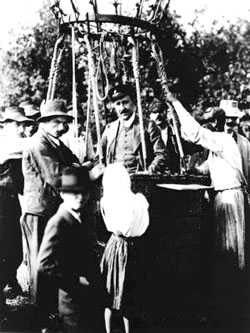
\includegraphics{intro/V-Hess-web_2.jpg}
	\caption{Victor Hess with his famous balloon, 1912.}
\end{marginfigure}

The field of \emph{astroparticle physics}, particle physics with cosmic accelerators, has been a fruitful source of mysteries in recent years. The existence of high-energy charged particles \emph{cosmic rays} was first demonstrated by Victor Hess in 191n, but their origin remains unknown over a century later. In that century, the ghostly neutrino particle was first proposed by Pauli in 192n, its existence was confirmed by in Y, its centrality in solar fusion was first posited by N, the solar neutrino flux was then measured in Z with at an unexpectedly-low rate (the so-called \emph{solar neutrino problem}), which then led to the first discovery of physics outside the Standard Model of particle physics, namely \emph{neutrino oscillations}. Experiments studying these solar neutrinos also accidentally provided us with the first case of observational astronomy with multiple 'messengers' (the observation of nearby supernova SN1987a with both neutrinos and photons), followed by the discovery of extra-terrestrial high-energy \emph{astrophyiscal neutrinos} with the IceCube detector in 2013 produced by the very same cosmic accelerators responsible for cosmic rays. A scramble to find the origin of these neutrinos led to the birth of a new field, \emph{neutrino astronomy}. The long-awaited discovery of Gravitational Waves by LIGO in 2015 was shortly thereafter followed by the discovery of a Binary Neutrino Star merger (GW170817) detected simultaneously with both photons and gravitational waves, kick-starting \emph{gravitational-wave astronomy}. One month later, the observation of a high-energy neutrino IC170922A from the direction of a flaring galactic nucleus led to the identification of the first likely source of high-energy neutrinos, TXS 0506+056. Thirty years after SN1987A, the year 2017 truly marked the dawn of an era of \emph{multi-messenger astronomy}. 


\begin{marginfigure}
	\centering 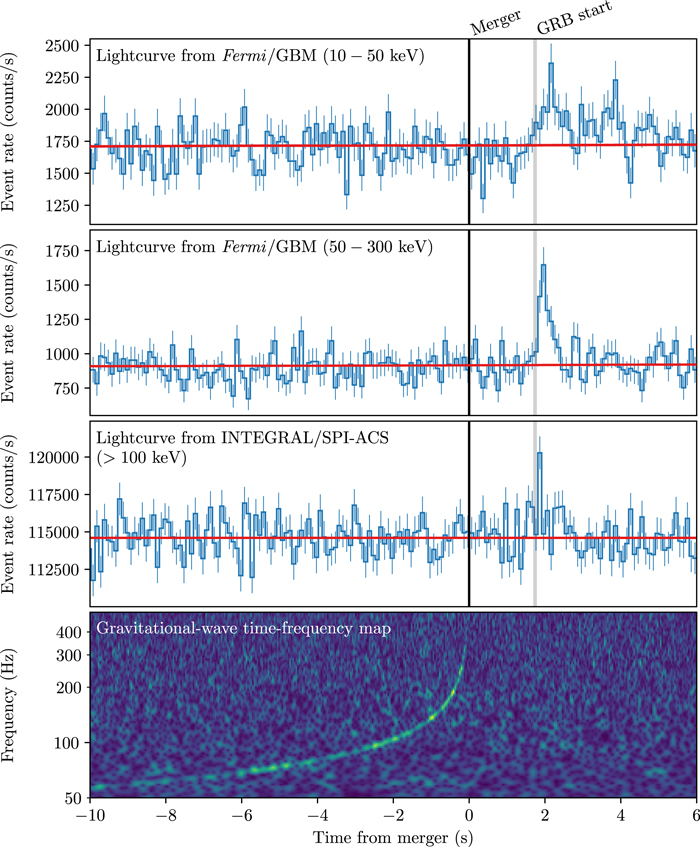
\includegraphics{intro/apjlaa920cf2_lr.jpg}
	\caption{The detection of a binary neutron star merger with photons (upper 3 panels) and gravitational waves (lower panel)  (from CITE).}
\end{marginfigure}

This thesis presents research probing the intersect of these new branches of astronomy with multiple messengers, incorporating searches for sources of neutrinos and gravitational waves using photons, and searches for photon sources using neutrinos. At its core, it seeks to understand what can be learned through combining knowledge from these new branches of astronomy with that of the oldest, namely photon astronomy as observed optical telescopes. The latter field is undergoing a revolution of its own, at the brink of transition from a mature human-driven field characterised by  of to an algorithm-driven one dominated by enormous data volumes. Optical astronomy is moving from object-centric to population-centric science, with scales at which detailed study of individual objects is becoming infeasible. In all three fields, a focus on rapid automated responses seeks to remove human-dependent latency in observational decisions, so-called \emph{realtime astronomy}. This drive was central in the identification of both GW170817 and TXS 0506+056, and forms a central part of this work.

This thesis begins with an introduction to ...




\setchapterimage[3.5cm]{mma/crab-page}
\setchapterpreamble[u]{\margintoc}
\chapter{Multi-Messenger Astronomy}
\labch{theory}
\begin{fquote}[William Shakespeare][Hamlet][1556] Though this be madness, yet there is method in it.
\end{fquote}

Multi-wavelength astronomy seeks to understand the universe through correlations between photons of different energies. Multi-messenger astronomy expands this concept to incorporate information from non-photon messengers, namely cosmic rays, gravitational waves and neutrinos. Each messenger provides a unique view of astrophysical processes in objects.

\section{Photons}

\begin{marginfigure}
	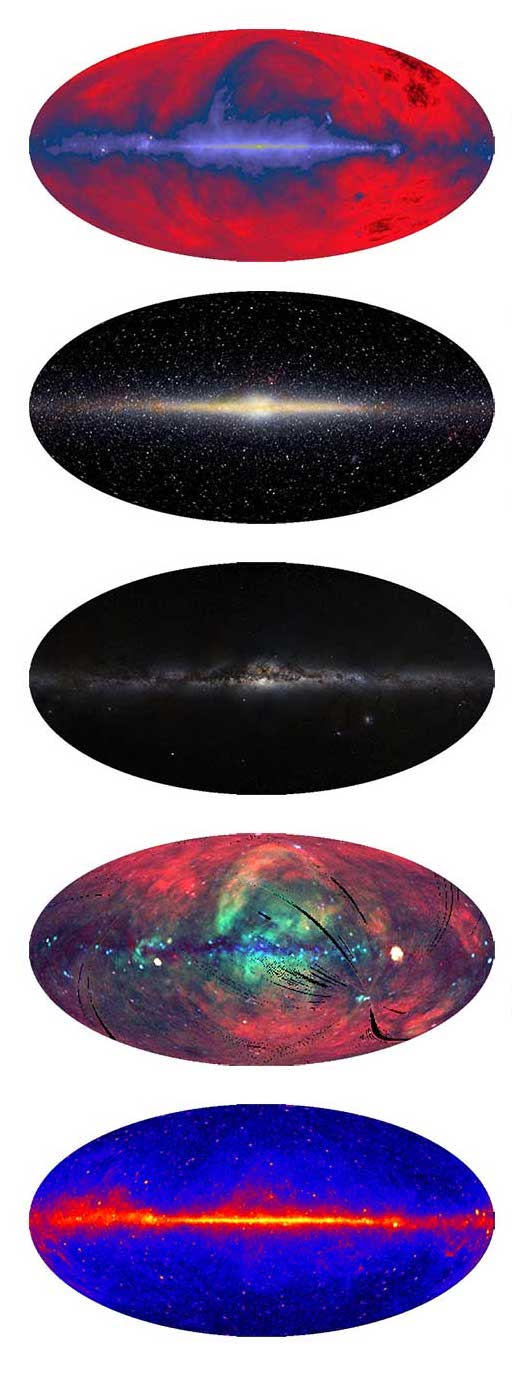
\includegraphics{mma/multiwavelength_sky_full}
	\caption{The sky, in galactic coordinates. From top: radio, infra-red, optical, X-ray and gamma-ray. Credit: NASA}
	\label{fig:mwsky}
\end{marginfigure}

Photon astronomy, in particular that in optical wavelengths, is the oldest branch of astronomy. As clear in Figure \ref{fig:mwsky}, our own galaxy is the most obvious structure at all wavelengths. The different pictures of the galaxy are also noteworthy. One example is dust extinction obscuring a large portion of the optical emission (middle panel), but  which is reprocessed to yield a particularly clear infra-red image (upper middle panel). This is an illustration of one broader principle, that interpolation between different photon energies can reveal .

In general, photon emission can be divided into two broad classes, \emph{thermal emission}
 and \emph{non-thermal emission}. Thermal emission is approximate black-bodies, and produces characteristic spectra. Non-thermal emission arises from particle acceleration, and is typically characterised by power-law emission. Objects can have both components. Thermal emission is typically centered in IR, optical or UV wavelengths, while non-thermal emission is typically manifested in both low energies (radio) and high-energies (hard X-rays and gamma-rays).
 
 \subsection{Thermal Photons}

 \subsection{Non-thermal Photons}
 
 \subsection{Spectroscopy}
 
While photon observations are typically integrated over relatively-wide rsange of wavelengths, additional information can be gleaned from \emph{high-resolution spectroscopy}, in which emission in fine wavelength bins can be analysed. With precision measurements  

\section{Cosmic Rays}

\emph{Cosmic Rays} were first discovered by Victor Hess in 1912 \sidecite{Hess:1912srp}. The name itself is a misnomer, as they are in fact charged particles. Being charged particles, they are deflected by magnetic fields, and it is thus challenging to determine where they originate from.

An industry of experiments has since developed to measure the composition and spectrum of Cosmic Rays, as illustrated in Figure \ref{fig:CR_spectrum}. The data is well-described by an unbroken power-law up to $\sim$1 PeV, beyond which there is a spectral softening known as \emph{the knee}. This softer spectrum continues before undergoing a hardening, known as the \emph{ankle}. There is then evidence of a high-energy cutoff, sometimes dubbed \emph{the second knee} in a case of metaphor-stretching.

\begin{figure}[!ht]
	\centering 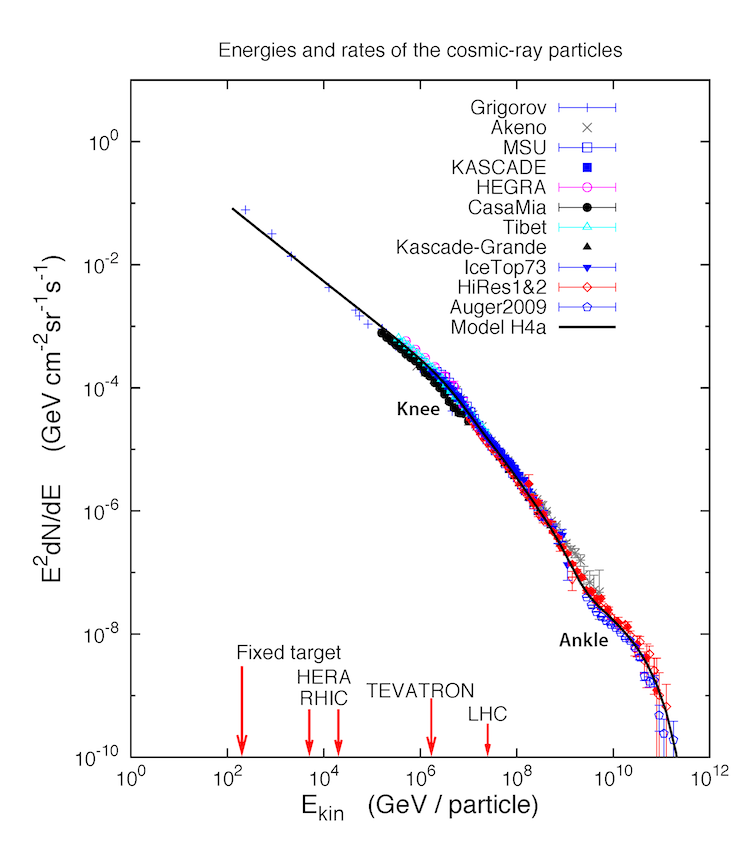
\includegraphics{mma/CRspectrum750}
	\caption{Cosmic Ray spectrum above 100 GeV, from x (icecube).}
	\label{fig:CR_spectrum}
\end{figure}

The knee is typically identified as the point at which cosmic rays transition from being predominantly galactic to extragalactic, with the ankle component being fully extragalactic. The origin of the high-energy cutoff is unclear, and the corresponding flux is so low that detector arrays must be several hundred square kilometers to study this regime with high statistics. As of 2020, this is primarily studied by the \emph{Pierre Auger Detector} and \emph {Telescope Array} detector. This regime is particularly interesting, because it is the point at which the GZK... mechanism 

UHECRs

\begin{equation}
p + \gamma_{CMB} \rightarrow \Delta^{+} \rightarrow n + \pi^{+}
\label{eq:GZK_pip}
\end{equation}
\begin{equation}
p + \gamma_{CMB} \rightarrow \Delta^{+} \rightarrow p + \pi^{0}
\label{eq:GZK_pi0}
\end{equation}

Equations \ref{eq:GZK_pip} and \ref{eq:GZK_pi0} would lead to a cutoff, in which pion production would suppress ultra-high energies above a threshold energy set by the mass of the $\Delta^{+}$ resonance. Attenuation would not occur for nearby cosmic ray sources, so the presence of such a cutoff would be evidence of an \emph{an extragalatic origin} for UHECRs. However, the \emph{Cosmic Ray Composition} determines the exact threshold for the GZK cutoff, with heavier comsic rays experiencing a much higher? threshold. There is thus much focus on understanding whether UHECRs are proton-dominated or Iron-dominated, with TA data supporting the former and PAO data supporting the latter. A joint working group concluded that these results are not in tension, once systematic uncertainties are accounted for. In summary, it appears that a definitive confirmation of a cutoff compatible with the GZK mechanism remains out of reach of present-generation instruments.

An alternative explanation for any apparent cutoff is that sources of UHECRs simply cannot accelerate particles beyond certain energies due to physical constraints. In general, any cosmic ray accelerator must at a minimum satisfy the \emph{Hillas Criterion} that any particle can be contained during the acceleration process \sidecite{1984ARA&A..22..425H}. This can be calculated by equating the Lamour Radius of a particle with the physical size of an accelerator:

Enu?

\begin{equation}
\frac{E_{\textup{max}}}{\textup{PeV}} \approx
1600 \times \frac{B}{\textup{Gauss}} \times \frac{R}{10^{16} \textup{cm}} \times
\beta Z
\label{eq:hillas}
\end{equation}

Equation \ref{eq:hillas} leads to a constraint on minimal magnetic field strength and source extension, which can be illustrated by a \emph{Hillas Plot} such as that in Figure \ref{fig:hillas_plot}.

\begin{figure}[!ht]
	\centering 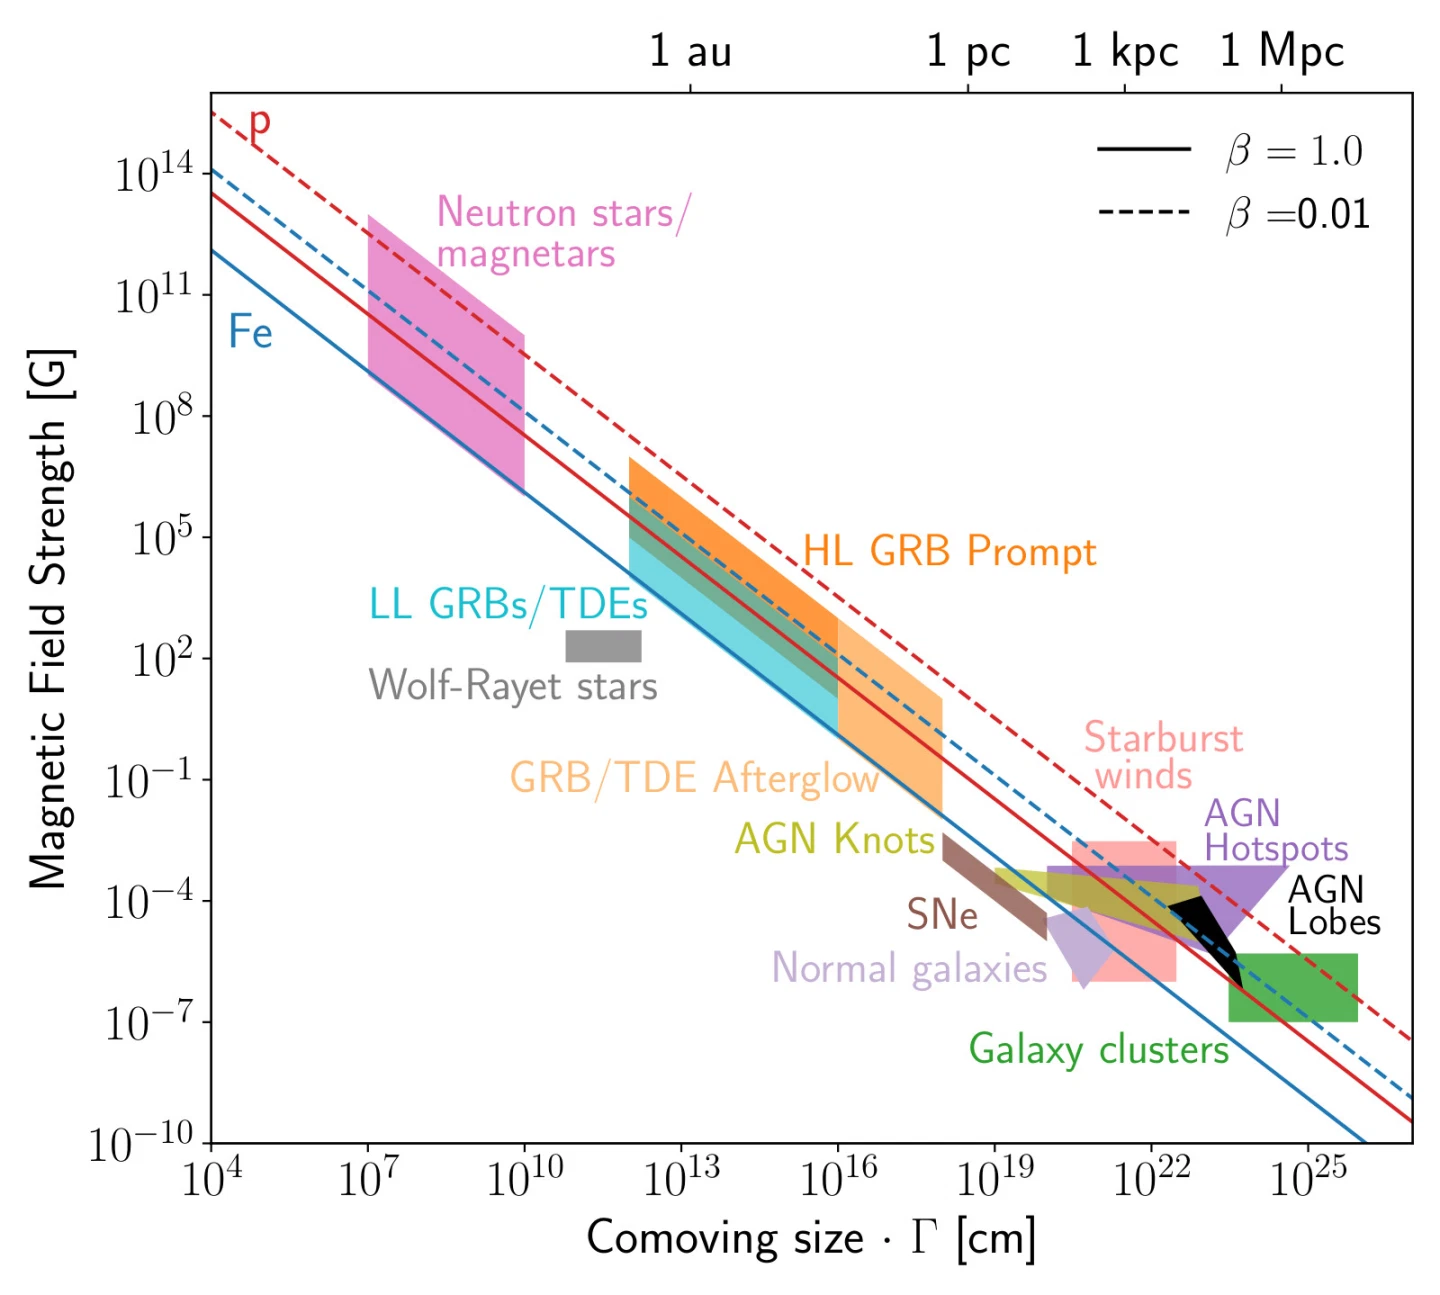
\includegraphics{mma/hillas}
	\caption{A Hillas plot illustrating possible cosmic-ray accelerators. credit: Mauricio B.}
	\label{fig:hillas_plot}
\end{figure}

Fermi acceleration

\section{Neutrinos}

The neutrino was first proposed as a particle by Pauli in 19xx as a solution to understand the mechanics of beta decay. Though observations suggested that the process involved a three-body decay, only the charged electron and proton could be measured. Invoking the existence of a light, chargeless particle provided a theoretical escape route. However, this particle was proven to be more than a theoretical construct, with the first evidence of observation by x in y.

In parallel, the \emph{Standard Solar Model} was developed in 19xx, which correctly identified that the sun was powered by nuclear fusion. This model came with a firm prediction of a guaranteed flux of electron anti-neutrinos, \emph{solar neutrinos}, which would be produced in tandem with thermal radiation. However, the first attempt to measure the solar neutrino flux, by the Homestake experiment in 196x, found a flux that was only half the predicted level. This deficit, dubbed the \emph{solar neutrino problem}, was subsequently confirmed by many other experiments.

The solar neutrino problem was finally resolved in 200n, when the electron neutrino deficit was conclusively matched with a corresponding excess of muon neutrinos. This confirmed the presence of \emph{neutrino oscillations}, by which neutrinos can change flavour states. To undergo oscillations, neutrinos must have different non-zero mass states, in contrast to previous assumptions in the Standard Model of particle physics. 

A new generation of experiments have developed to probe neutrino flavour oscillations across a range of energies, baselines and channels. In general, \emph{reactor neutrinos} are used to probe electron neutrino disappearance, while solar neutrinos are used to probe muon neutrino appearance. Our current knowledge is summarised in N. Only the difference in squared masses can be probed by these experiments, so while it is known that mass states 1 and 2 have a difference of neV, and 13 $\sim$neV, the absolute ordering could be either \emph{Normal ordering} (m1<m2<m3) or \emph{inverted ordering} (m3<m1<m2). Directly measuring these masses remains a particle physics aim, with recent experiments such as KATRIN probing the sub-eV regime. IceCube has provided the first evidence of neutrino oscillations over astronomical baselines, with the detection of astrophysical tau neutrinos.

In 1987, experiments studying the solar neutrino problem unexpectedly measured a simultaneous excess in neutrinos. This detection occured shortly before the discovery of a nearby supernova in the L? Magellanic Clouds, and coincided with the core-collapse of that supernova. These \emph{supernova neutrinos} were the first that could be cleanly identified as arising from beyond our solar system, and confirmed the essential \emph{neutrino cooling} that is required during the stellar core collapse. This was also the first example of astronomy with multiple messengers. Only nearby galactic supernovae produce a sufficiently large flux to be clearly identified against this background. However, the predicted diffuse supernova neutrino background will soon be within reach of experiments.

Interactions of cosmic rays with the atmosphere produce a guaranteed flux of \emph{atmospheric neutrinos}, and this was finally confirmed observationally with the AMANDA detector in 200n. This flux extends over many orders of magnitude,. It is expected that there should be a distinct second \emph{atmospheric prompt} component of neutrinos, produced via charm quark in the atmosphere. However, this component has not yet been measured.

\emph{Astrophysical neutrinos} are to some degree guaranteed as a byproduct of high-energy cosmic ray production, resulting via pion production from the interaction of cosmic rays with ambient matter (pp) and radiation (p$\gamma$). However, the extent of astrophysical neutrino production depends very substantially on the conditions at cosmic ray accelerators, with high fluxes requiring abundant target material for pion production. A flux of astrophysical neutrinos was first discovered by IceCube in 2013, at a level close to the maximal one. This astrophysical component begins to dominate over the atmospheric neutrinos above n TeV. No neutrino source has yet been discivered, but possible sources of these astrosphysical neutrinos are discussed further in Chapter N.

At the very highest energies, it is expected that the impact of the GZK cutoff (Equations \ref{eq:GZK_pip} and \ref{eq:GZK_pi0}) should generate a flux of neutrinos through interactions of UHECRs with the cosmic microwave background. These \emph{Cosmogenic Neutrinos} have not yet been observed, but upcoming radio neutrino observatories in particular are seeking to measure them. The flux of cosmogenic neutrinos depends very strongly on the composition, density and evolution of cosmic ray sources, so it remains unclear whether it will be accessible to these detectors. (See Fig N)

\begin{figure}[!ht]
	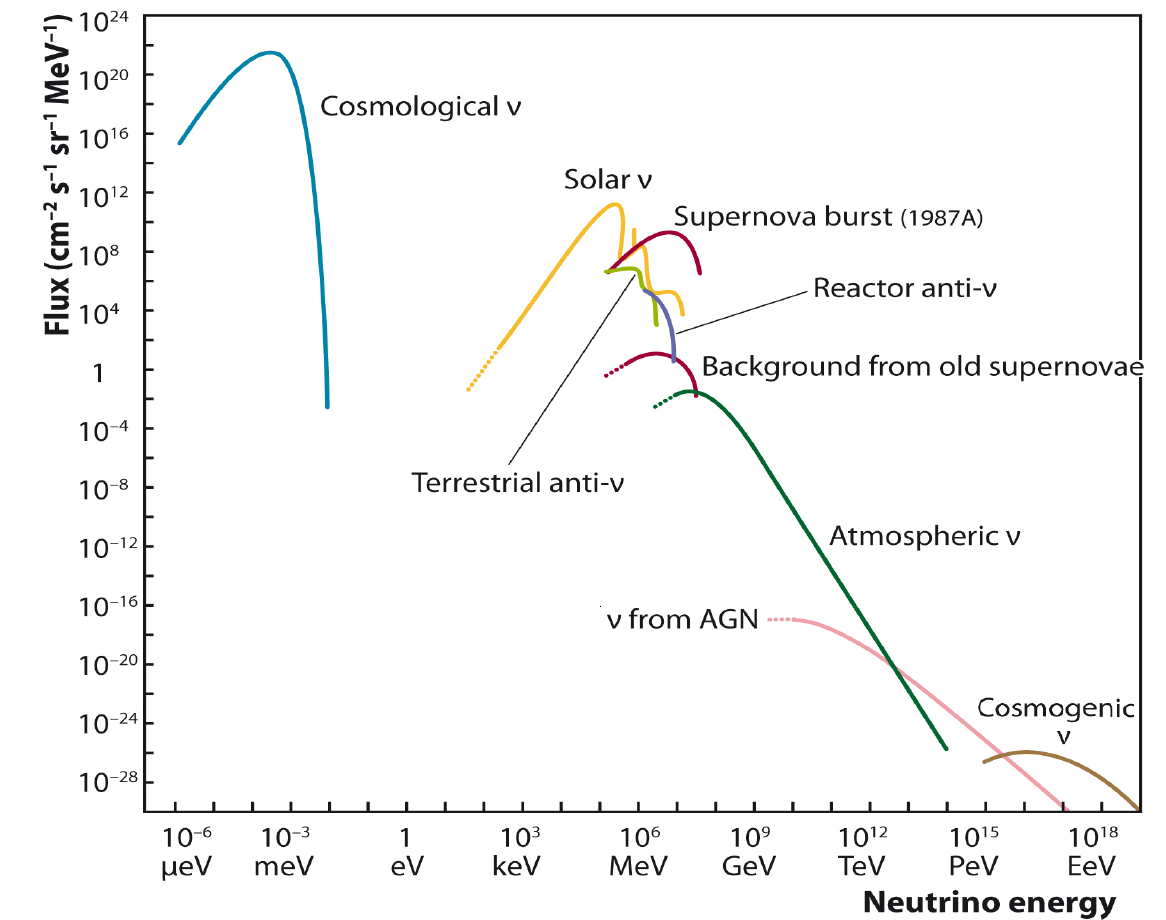
\includegraphics{mma/nu_spectrum}
	\caption{The full spectrum of neutrinos, from all sources. Credit: IceCube}
	\label{fig:nu_spectrum}
\end{figure}

\begin{figure}[!ht]
	\centering 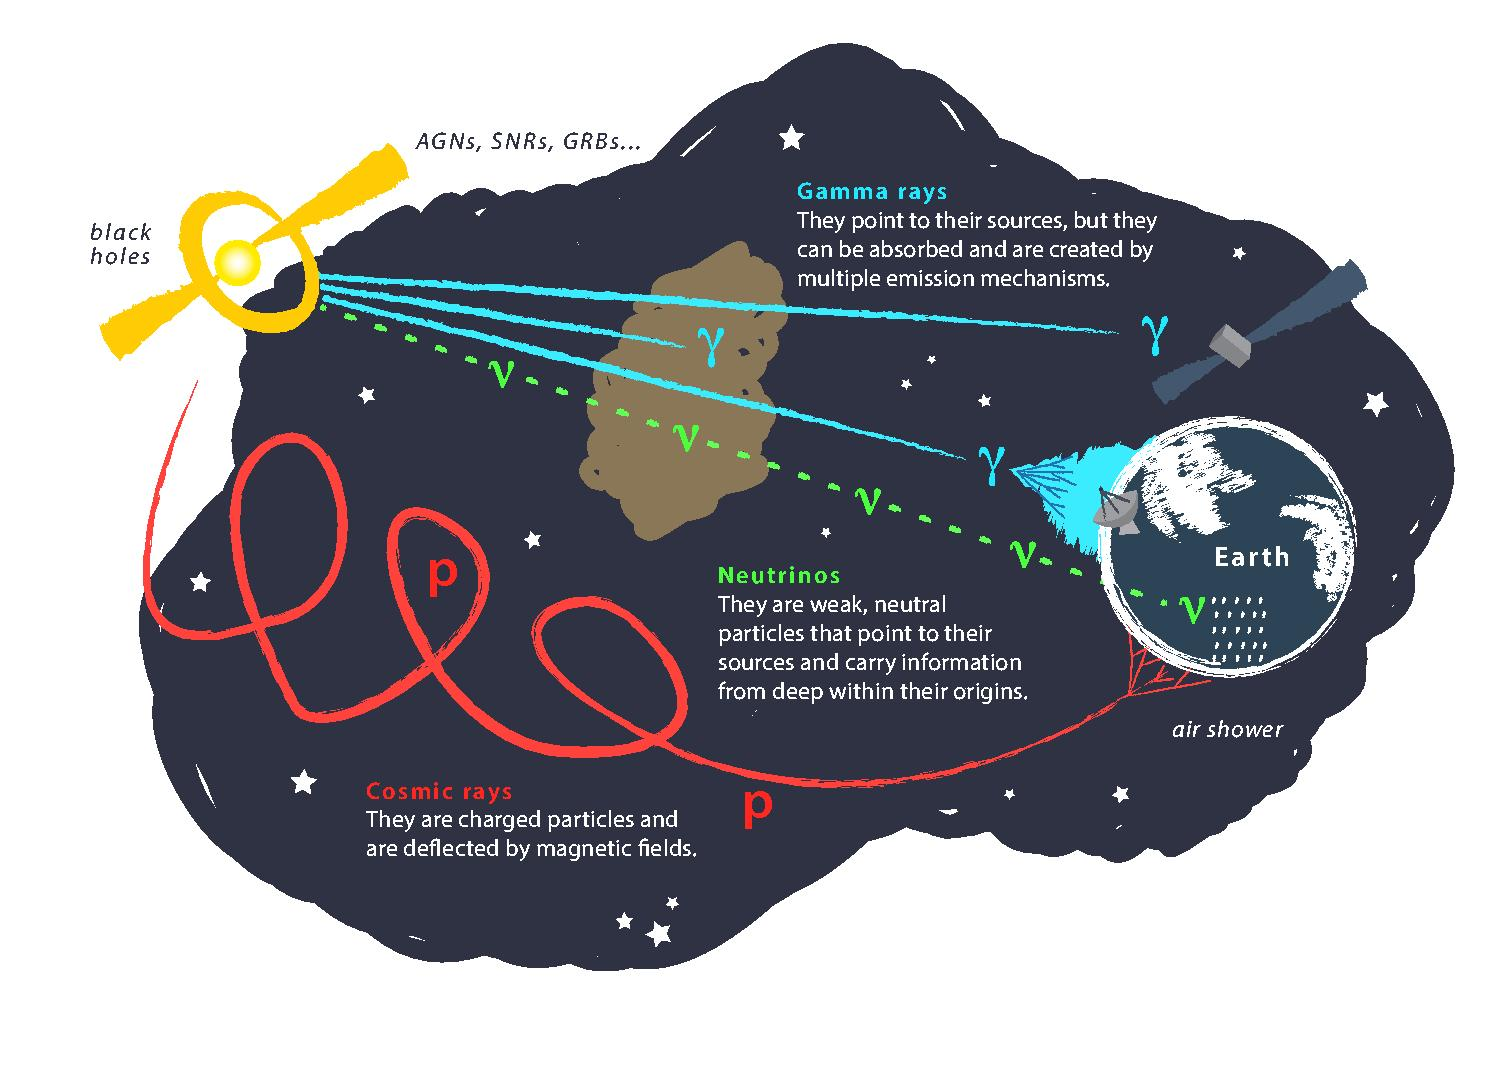
\includegraphics{mma/mm}
	\caption{An overview of multi-messenger astronomy. credit: IceCube.}
	\label{fig:mm}
\end{figure}

cosmological

In all cases, neutrino production is accompanied by a flux of pionic gamma-rays. However, these can be subsequently absorbed, so neutrinos may be produced in seemingly gamma-dark sources.

Waxmann-Bachall.

glashow

\section{Gravitational Waves}

Einstein
LIGO
LISA
other sources?
quadropole moment
supernovae
Einstein Telescope
O4
\setchapterimage[8.5cm]{desy_blazar}
\setchapterpreamble[u]{\margintoc}
\chapter{Sources of astrophysical neutrinos}
\labch{sources}
\begin{fquote}[Winston Churchill][Lady Windermere's Fan][18??]...man will occasionally stumble over the truth, but usually manages to pick himself up, walk over or around it, and carry on. 
\end{fquote}
As far back as X, when nuclear fusion was proposed as a mechanism to power the sun, it was expected that a flux of solar neutrinos should be detectable on Earth. This prediction was confirmed by early neutrino detectors, ZZ and Z, which measured the flux xyc.
The discovery of a source of neutrinos from beyond the solar system followed soon after, with the detection of nearby supernova SN1987A. Nearby supernova occur either within our galaxy, or in the neighbouring Magellanic clouds, at a rate of a couple per century. In thie case of SN1987A, the detection of the supernova was preceded by simultaneous detections of an elevated neutrino flux in multiple detectors on Earth. The coincident detection of photons and neutrinos marjked the first multi-messenger detection of an astrophysical source.

It is now well-understood that there is a diffuse flux of MeV-neutrinos produced from SN?, and preparations are underway for the inevitable next nearby SN, coordinated by the SuperNova Early Warning System (SNEWS). Given the increased volume of current-generation neutrino detectors, the next nearby supernova will be measured with much greater precision. IceCube itself will contribute to this, through a dedicated supernova detection system. Given the detector geometry, IceCube will not be able to identify individual neutrino events, nor reconstruct their directions. However, an increase in DOM noise will be clearly measurable, and likely with sufficiently resolution to resolve the time-evolution of the signal. 

In both cases, the neutrinos detected at MeV-energies.  However, in light of the discovery of a flux of high-energy astrophysical neutrinos by IceCube, a new branch of astronomy has developed searching for sources of these astrophysical neutrinos. The central fact for neutrino astronomy, at least in the ~TeV-PeV range for which IceCube is sensitive, is that at lower energies there is an overwhelming background, while at higher energies, statistics are poor. This is illustrated in Fig. The power of IceCube to detect an astrophysical flux depends on the degree to which this differs from the atmospheric background. Above all, the expected energy distribution for most astrophysical sources likely differs from the soft-spectrum atmospheric neutrino flux. In addition, the spatial distribution of the background is broadly isotropic, and uniform as a function of right ascension. The temporal distribution of this background, beyond small-scale season variations, is also reasonably isotropic. Foreground fuxes which differ substantially will be most easily detected.

The expected degree of anisotropy in the extragalactic astrophysical neutrino flux strongly depends on the properties of the assumed sources, in particular their density and source evolution. The source evolution describes the rate or density evolution of astrophysical objects as a function of redshift. For sources with a negative source evolution, the density in the local universe is greater than at high redshift, so there are fewer neutrinos produced by distant, unresolved sources. Conversely, for a strongly positive source evolution, we expect a greater fraction of neutrinos to arrive from unresolved sources. When local density and source evolution are coupled, we then find arrive at a flux which anisotropic to varying degrees. Given that the atmospheric backgrounds are broadly isotropic, and uniform as a function of right ascension, the sensitivity of IceCube to a given astrophysical flux will depend strongly on whether that flux is sufficiently spatially anistotropic to distinguish it from atmospheric backgrounds. A higher-density source population, with positive evolution, would be much harder to identify that a low-density one with negative evolution. Anisotropy in neutrino arrival times can be an additional metric to distinguish astrophysical neutrinos. For sources which are variable or transient, neutrino emission is only expected for distinct time periods, eliminating background events.

In general, given knowledge about the background, the most agnostic methods to identify neutrino sources look for clustering within the data without reference to external datasets. Such auto-correlation analyses can be done with either a time-integrated or time-dependent all-sky likelihood scan. The result of such an analysis is a pixelised likelihood map. Comparisons of this map can then be made to expectations from background, either using the single "hottest spot" in the sky, or by comparing the distribution of hotspots. No significant excess was found for either approach, providing significant general constraints on neutrino source populations, . Given the current detector volumes and resolution, as well as the lack of observed lower-significance overfluctuations, it appears that the astrophysical neutrino flux is not sufficiently anisotropic for auto-correlation analyses to discover a neutrino source in the near future.

As an alternative to agnostic searches, specific source hypothesis tests can be substantially more sensitive. Given the position of a known astrophysical object, the threshold for a significant excess is greatly reduced due to the avoidance of an all-sky trial factor. Sensitivity can be further enhanced when information from multiple objects is combined in a so-called 'stacking search'. These methods can be used to test for neutrino excesses correlated to astrophysical populations. One drawback of these methods is that their sensitivity strongly depends on the quality of available multi-wavelength data. Often these catalogues are not complete, particularly in the case of transient or variable objects. 

On the other hand, realtime analysis is a complementary method that inverts this traditional object neutrino relationship. Instead of taking a known object, and asking whether neutrinos are correlated to it, realtime analysis identifies likely-astrophysical neutrinos and seeks to identify coincident astrophysical objects that could potentially have produced the neutrino. The power of realtime searches is that they can, if a possible counterpart is identified, lead to contemporaneous multi-wavelength follow-up that maybe reveal more about a given object. Within this context, the 

However, it should be noted that both realtime and stacking analyses are only sensitive to cases where neutrino sources have detectable EM counterparts. It might however be the case that EM emission from neutrino sources is either absorbed or attenuated, and consequently stacking analyses will be unable to identify such EM-dark neutrino sources. Furthermore, particularly for CCSNe-like populations following the Star Formation Rate (SFR), a large fraction of the astrophysical neutrino might in fact come from unresolved sources.

\section{Galactic Neutrino Emission}

As can be seen in Fig, the galactic plane accounts for a significant fraction of EM emission in every wavelength, from radio to high-energy gamma rays. It is therefore natural to suspect that the Milky Way might contribute to the astrophysical neutrino flux. Likely sources of galactic neutrinos are much the same as high-energy gamma rays, namely Supernova Remnants (SNRs) and Pulsar Wind Nebulae (PWNe). In addition, given that the galaxy should act as a target for extragalactic UHECRs and thus produce secondary neutrinos, it is guaranteed that some galactic contribution should be present in the neutrino flux. Despite this expectation, to date no significant galactic neutrino excess has been found. Given the position of the galactic center in the southern hemisphere, where IceCube muon track datasets are less sensitive, IceCube searches are typically conducted using likely-astrophysical cascades. These searches have in some cases been conducted jointly with the northern-hemisphere ANTARES neutrino observatory, and additionally with HAWC high-energy gamma-ray detector. At this point, limits on the galactic neutrino flux are beginning to constrain reasonable models, above all the standard KRA-$\gamma$ model. Given constraints limiting the galactic contribution to less than n\% of the diffuse flux, we can state with certainty that the astrophysical neutrino flux must be \textbf{predominantly extra-galactic}. 

Specific tests were performed on likely galatic sources of high-energy neutrinos, but none have identified any specific excess. The latest constraints limit the contributions of PWNe and SNRs to be less then Y\% amd Z\% respectively. 

An additional analysis was performed on the Fermi Bubbles, a large gamma-ray-emitting region perpendicular to the galactic plane. The origin of the Fermi Bubbles is still unclear, but one explanation is X. Neutrino emission might be expected from XYZ, however no excess was found. 

Fermi Bubbles
\section{Emission from the Local Universe}
As with the galactic plane, it is expected that collisions between UHECRs and matter in the local universe should produce a secondary flux of high-energy neutrinos, regardless of the ultimate origin of the UHECRs. Additionally, the primary flux of astrophysical neutrinos might well be correlated with the local matter density of the universe, for example in cases where neutrinos are produced from X, Y or Z. Both cases were tested through a correlation analysis between neutrinos and local matter density as defined by the 2-mm Redshift Survey (2MRS) catalog. 
2MRS survey and stuffs.

\section{Blazars}
One long-favoured candidate neutrino source class is Blazars, the subclass of Active Galactic Nucleii (AGN) with relativistic particle jets that point towards the Earth. These blazars have long been known to emit both high-energy  and Very-High Energy (VHE) gamma-rays in the MeV-TeV range. Extensive modeling of these objects, particularly nearby examples such as BL-Lac and Markarian 421 (Mrk 421), have revealed a characteristic SED with two charectiristic "humps", as shown in Figure n. While there is consensus that the lower-energy hump likely arises from synchrotron emission,  the higher-energy one has been explained both by leptonic and hadronic models. Neutrino emission would be expected for the latter in all cases, but never the former.

Since 200n, there have been extensive observations by the Fermi Large Area Telescope (Fermi-LAT), an MeV-GeV gamma-ray satellite telescope. With a significantly increased sensitivity over its predecessors, Fermi has discovered n00 blazars as of 4FGL, adding to the  n from previous mission.

It is now known that blazar emission dominates the high-energy gamma-ray sky. Modelling of the "Extragalactic Background Light" (EBL) typically assumes that 80\% of all gamma-ray emission in the Fermi range is produced by blazars. IACTs have also confirmed that blazars sunch as Mrk 421 are extremely bright at TeV gamma-rays. Although photons at these energies are quickly attenuated during propagation due to interactions with CMB PHOTONS, it is assumed by extrapolation from observations of nearby blazars that more distant ones are also likely TeV-emitters.

 Given the simultaneous production of gamma-rays with neutrinos in hadronic interactions, it is natural to suspect that bright gamma-ray sources, namely blazars, may additionally be neutrino sources. This hypothesis has been tested repeatedly by IceCube, and under the assumption of a linear proportionality, the contribution of all blazars has been constrained to less than 6\% of the astrophysical neutrino flux. This limit additionally accounts for the contribution of unresolved blazars, as well as those in the 3FGL? catalogue that were tested. A more agnostic search on 3FHL blazars constrained their contribution to be less than 20-30\%, without limiting the contribution of unresolved blazars. In both cases, it must be pointed out that this limit is dependent on assumed spectral index. These constraints generally disfavoured blazars as neutrino sources, with fine-tuned models required to generate neutrinos from lower-luminosity unresolved blazars without violating constraints on the brighter resolved blazars. 
 
 \subsection{TXS 0506+056}
 
 However, this interpretation was challenged by the observation of IC170922A, a high-energy neutrino that arrived in spatial and temporal coincidence with a bright gamma-ray flare from blazar TXS 0506+056. A likelihood analysis correlating high-energy neutrinos with the monthly gamma-ray lightcurves of Fermi blazars led to the disfavouring of a chance coincidence at the level of $3 \sigma$. This result implied that, rather than the average gamma-ray flux, high-energy neutrinos might instead be correlated with instantaneous gamma-ray flux. Prompted by this observation, the IceCube collaboration conducted a time-dependent search for archival neutrino emission from the direction of TXS 0506+056, and identified a signal-like neutrino cluster in 2014-15 with a significance of $3.5 \sigma$. Surprisingly, this neutrino cluster was not accompanied by any significant contemporaneous gamma-ray activity CITESIM. TXS 0506+056 thus presented a somewhat contradictory picture, with both pieces of evidence challenging to interpret in a unified framework. Theoretical attempts to model the arrival of IC170922A were generally successful, particularly when accounting for the likely Eddington Bias in any flux estimation . However, attempts to model the arrival of the neutrino cluster were significantly more challenging as the implied neutrino flux was much greater than the measured gamma-ray flux. Despite relatively poor observational constraints for the 2014-15 period, there have been no successful models describing all claimed neutrino emission from TXS 0506+056.
 
 In general, how to resolve the apparent incoherence of these observations remains an open question. Additionally, it remains unclear whether or how TXS 0506+056 is, in some way, "special". If it were simply one of many neutrino blazars emitting proportionally to its gamma-ray flux, we would have expected the stacking analysis to identify a correlation with higher significance.  On the other hand, if the source is in some way unique, then the observed behaviour would be more coherently understandable. One study promptly identified that the hitherto-accepted classification of TXS 0506+056 as a BL-Lac was incorrect, and it was in fact an FSRQ. As a member of the rare subclass of 'masquerading BL-Lacs', it had a specific properties which in some models would indicate enhanced neutrino emission. There has been some recent evidence that TXS 0506+056 has a unique jet geometry, citeBRITZEN, but there is to date there is no model which has attempted to connect this geometry to observations of neutrino emission. A search for additional neutrino clusters from blazars in 4FGL did not reveal any significant excess correlation with either FSRQs or BL-LACs.
 
 \begin{figure}[!ht]
 	\centering 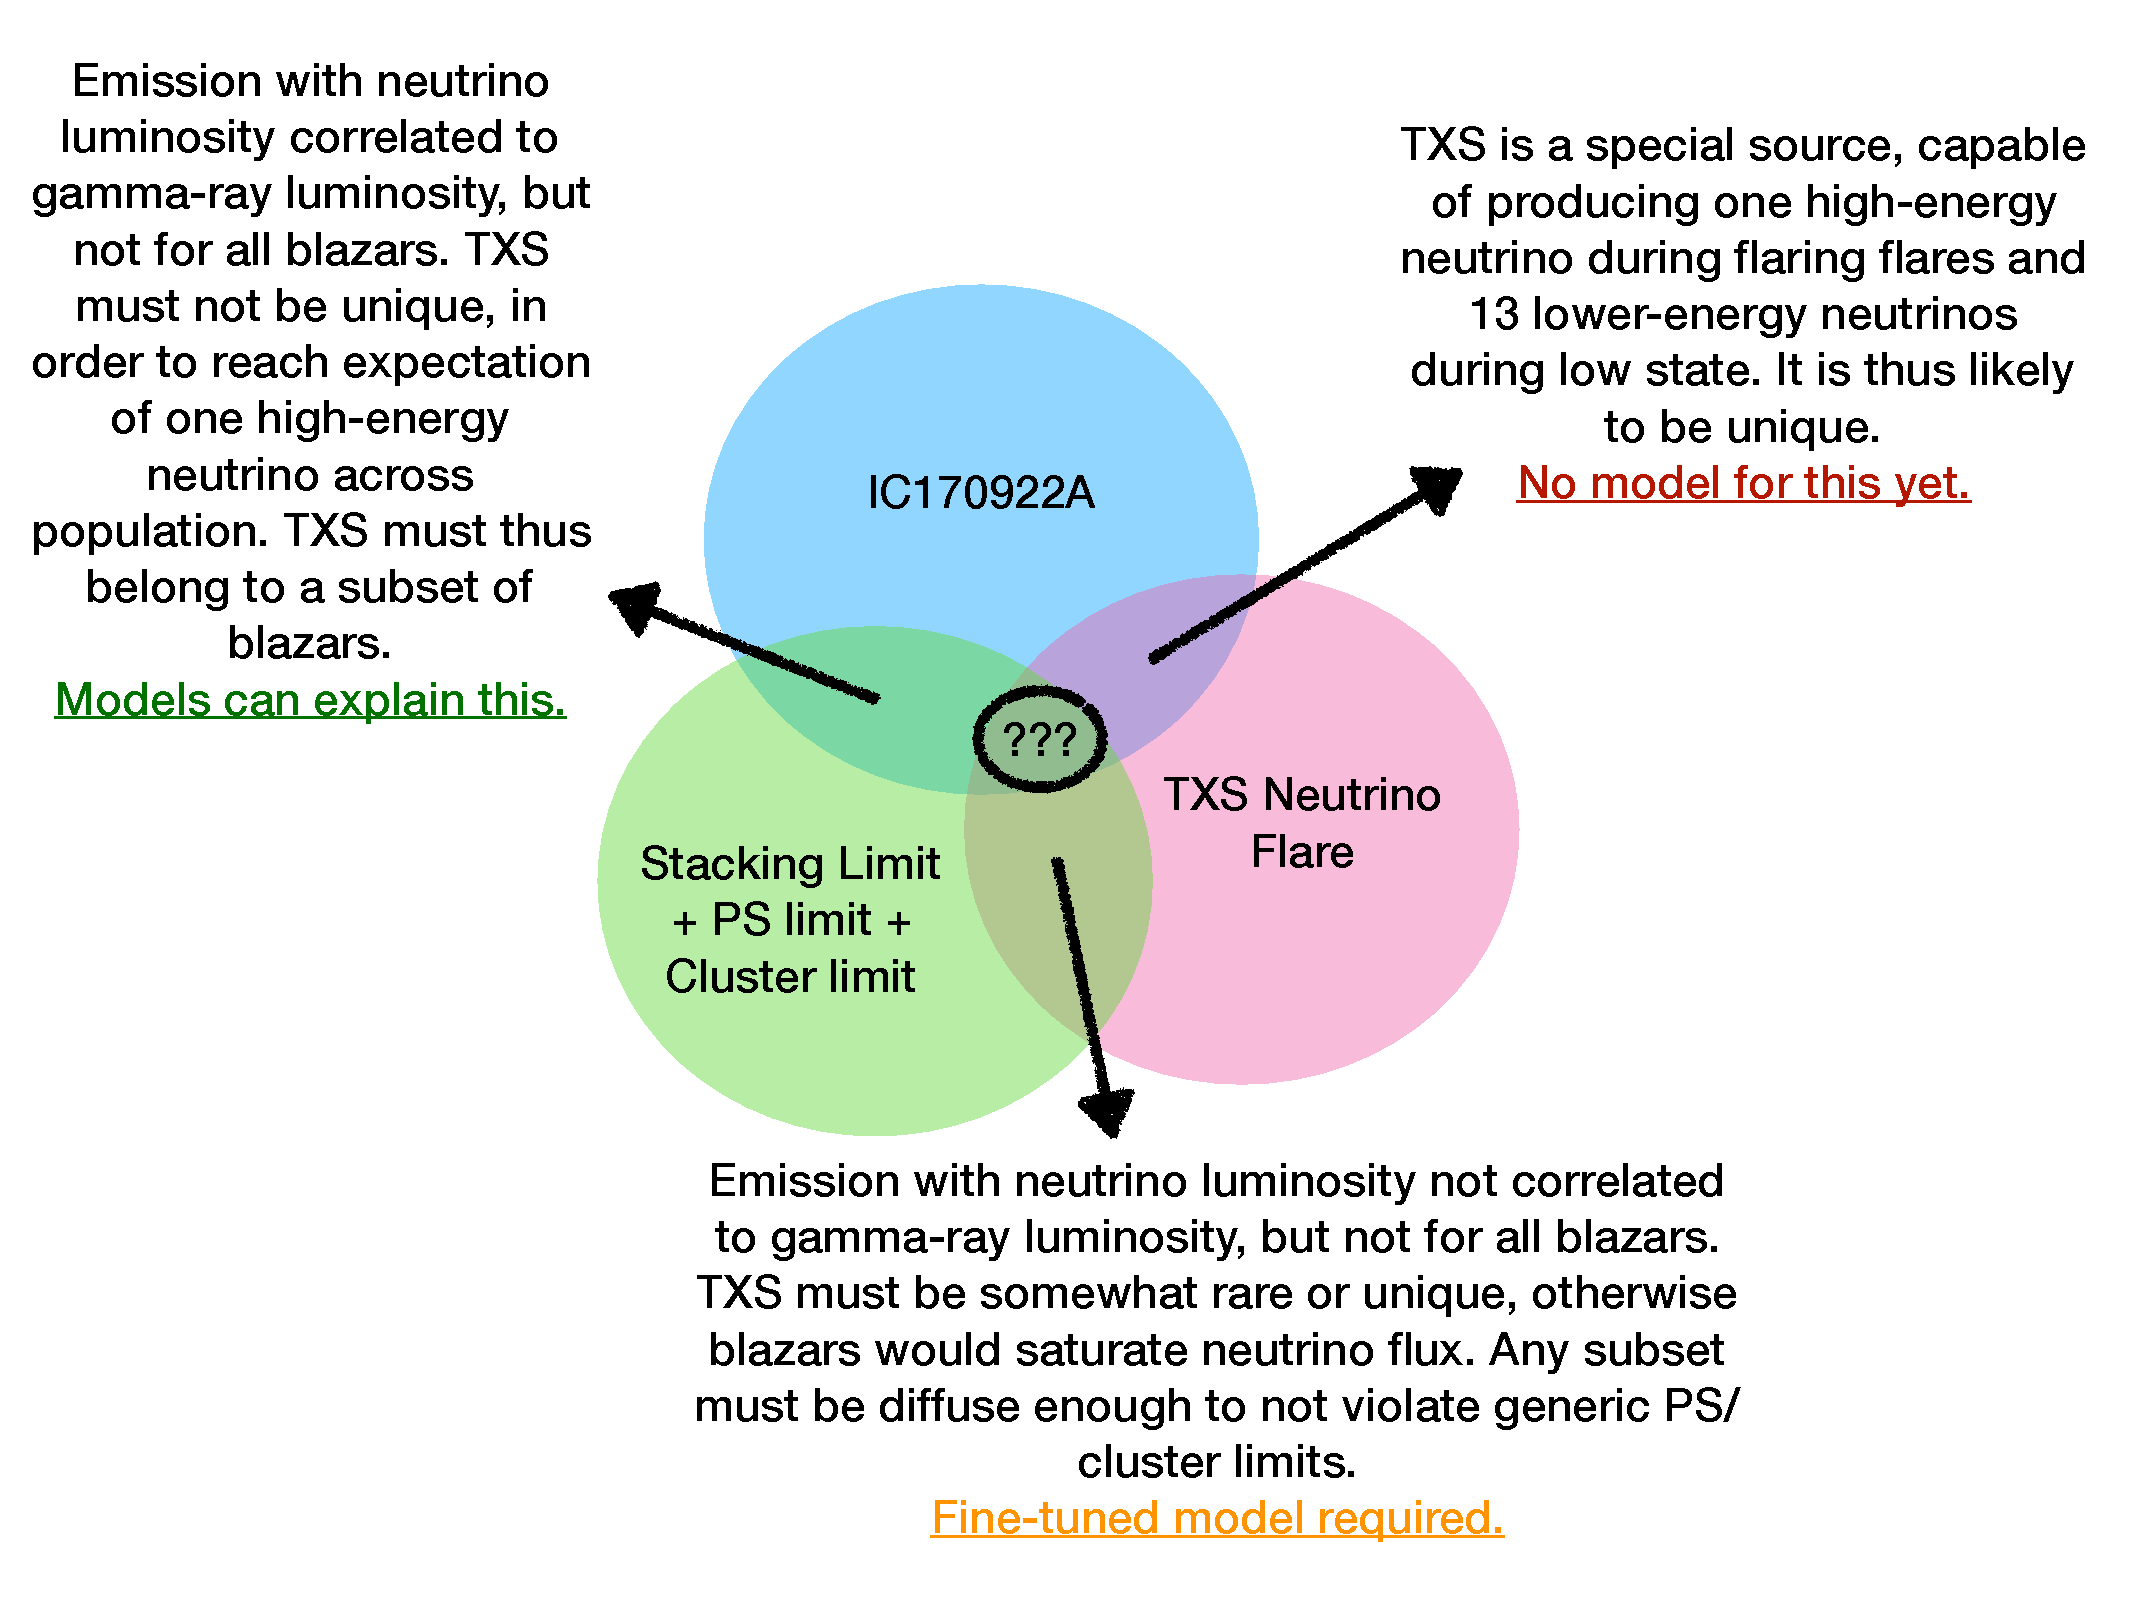
\includegraphics{txs_logic}
 	\caption{The challenge of coherently understanding the scenarios for neutrino emission from blazars, given the two pieces of evidence from TXS 0506+056, as well as the constraints from IceCube stacking analyses, general point-source searches and generic time-dependent cluster searches. To date, no model has resolved all three observations coherently.}
 	\label{fig:TXSLogic}
 \end{figure}
\section{Gamma-Ray Bursts}

Gamma-ray Bursts (GRBs) have long been proposed as a source of neutrinos. GRBs themselves fall into two broad categories, short and long, which are believed to arise from distinct physical populations. Long GRBs have been associated with the appearance of broad-lined type Ic supernova, and are thus believed to arise from a relativistic jet produced during supernova explosion. 

Short GRBs are now known to arise from relativistic jets launched during the merger of binary neutron stars. The first, and to date only, observed coincidence occurred for the gravitational wave event GW170817, which was associated with the short GRB 170817A and the kilonova AT2017gfo. Observations of GRB170817A revealed that it was particularly underluminous relative to most short GRBs, a fact later explained by comprehensive observations and modelling of AT2017gfo that confirmed an off-axis jet geometry. Given the relatively narrow jet opening angle, it is expected that the majority of future binary neutron star mergers detected by LIGO will not have detectable GRB counterparts.

Afterglow for both?

For both short and long GRBs, neutrino emission might be expected during the so-called "prompt phase" of gamma-ray emission. IceCube has undertaken numerous searches for neutrino emission, but has so far observed no correlation. Prompt emission from GRBs is particularly favourable for neutrino detection, because the brief and well-defined search period greatly reduces the expected background for such searches. This scenario is indeed one of the most-constrained by IceCube, which current limits restrict to less than 1\% of the astrophysical neutrino flux. 

Our understanding of GRBs has recently expanded further after the discovery of GRB VHE gamma-ray emission by MAGIC and HESS collaborations. The timescales for this emission, extending as much as 18 days after prompt phase indicates that high-energy processes extend throughout the so-called afterglow phase. consequently there is renewed focus on potential neutrino afterglow  emission, which is significantly less-constrained. One previous Icecube analysis limited the contribution to n\% (cite HESE).

An additional subclass are so-called low-luminosity GRBs (LLGRBs), believed to be... Given the poor efficiency with which source sources are detected, stacking searches of LLGRBs are significantly less powerful. However, for this case, generic searches for short-scale neutrino multiplets provide constraints on the contribution of such a population. In this case, they are known to contribute less than x\%.
\section{Core-Collapse Supernova}
 \begin{marginfigure}
	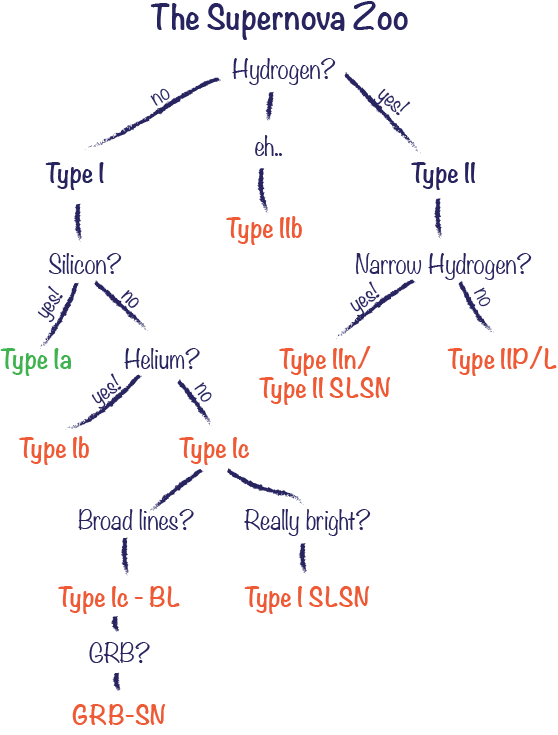
\includegraphics{sn_zoo-1}
	\caption{An overview of the current supernova classification scheme, which has been recently expanded to include superluminous supernova. Type 1a supernovae, marked in green, arise from thermonuclear explosions. All other classes, marked in origin, occur due to core collapse.}
	\labfig{fig:snzoo}
\end{marginfigure}
Supernovae, the explosive death of stars, are perhaps the best-studied phenomenon in astronomy. They are traditionally classified based on observed properties, rather than intrinsic physical attributes. An overview of a classification scheme is given in Figure \ref{fig:snzoo}. The most fundamental distinction is in explosion mechanism, with Type 1a SNe occuring due to thermonuclear explosions while all other classes are believed to arise from stellar core collapse. Further distinctions are made based on emission line, yielding the classes of Type Ib, Ic and Type II. Some SNe are observed to have narrow lines, which occur due to interaction with ejecta and circumstellar material (CSM). These supernova are denoted with 'n', the most common being Type IIn. This group in particular are candidate neutrino sources, in which neutrinos are produced via CSM interactions. An additional class of SNe is the IIP subclass, the subset of Type II SNe for which a characteristic lightcurve plateau is observed. Such plateaus are typically assumed to arise from....
Those Type II supernova not falling into IIp are instead classified as IIL, with characteristic Linear decay lighcurves.

Type Ic SNe can occasionally be observed with spectroscopic features known as Broad-Lines, which typically indicate the presence of fast-moving material. These form a distinct sublass, and it is this subclass which has been associated with long GRBs. Though radio observations have excluded the possibility that all Ic-BL SNe host relativistic jets? it is expected that even those without an observed GRB may instead host so-called 'choked jets' . These occur if a relativistic jet is lauched during core collapse, but because it lacks sufficient power to break through the outer layers of stellar material, it is stopped within the interior of the star. These choked jets, much like their standard counterparts, could produce neutrino emission. This scenario is however particularly difficult to test, because only those choked jets aligned towards Earth would produce a neutrino signal. As the alignment of a choked jet cannot be measured, it is impossible for us to say which supernova should or should not produce neutrinos. 

An additional category of supernovae has been recently observed, identifiable by their atypical brightness. So-called Superluminous supernovae (SLSNe) were initially classified as any SNe with an absolure magnitude brighter than -21 mag. However, in recent years, increased study has led to a spectroscopic classification being favoured, with some dimmer objects in the range $-20 < M < -21$ also being accepted. There are currently two favoured models to explain why SLSNe are so bright, namely the Magnetar model and the PISN model. .....

\section{Tidal Disruption Events (TDEs)}
== Roche Limit==
The tidal radius can best be understood by comparison to the more straightforward concept of the Roche Limit, otherwise known as the Roche Radius. The Roche Radius is defined as the distance at which the self-gravitiational force acting on the outer surface of a body are exactly equal to the gravitational pull of a second body on that same mass element. If a star moves closer than its Roche Radius for an SMBH, there will be a net force on mass elements on the star surface towards the SMBH, and the star will disintegrate.

The Tidal Force of one body acting on another is simply the difference in gravitational force strength between the closer surface of the sphere and its core. The Tidal Force of a black hole of mass M and distance d, acting on a mass element u lying on the closest point of the stellar surface, is thus given by:

$F_{tidal} = \frac{GMu}{(d-r)^{2}} - \frac{GMu}{(d)^{2}}$

$F_{tidal} = \frac{GMu}{d^{2}}((1-\frac{r}{d})^{-2} - 1 )$

Using Binomial Expansion with the reasonable assumption that r<<d, we reach an approximation:

$F_{tidal} \approx \frac{GMu}{d^{2}}\times \frac{2r}{d}$
The Roche Radius for a black hole of mass M for a star of mass m and radius r is thus found by equating this with the self-gravitational force acting on the same mass element. 

$F_{grav} = \frac{Gmu}{r^{2}} = \frac{2GMur}{d^{3}} \approx F_{tidal}$

$ d = r \times (\frac{2M}{m})^{\frac{1}{3}} \approx r_{roche}$

== Tidal Radius ==

This simplistic model does not hold for Tidal Disruption Events. The tidally-disrupted body would need to be in a circular orbit with synchronised spin, but stars tend to have approach Black Holes parabolically. In addition to Angular Momentum, General Relativity should be accounted for. This is particularly relevant for large black holes. A rigorous definition of Tidal radius should account for these things, but in any case, the point at which a star becomes 'tidally disrupted' is difficult to define. An event which only strips a fraction of the outer shell of the star would be ambiguous. Fortunately these definitions differ only by the order of unity from the Roche Radius. In the original paper introducing these calculations by [https://www.nature.com/nature/journal/v333/n6173/abs/333523a0.html Rees (1988)], the tidal radius was defined as the radius at which the mean internal density of the star is exceed by the mean internal density of the orbital volume. In this definition:

$\rho_{star} = \frac{m}{\frac{4}{3} \pi r ^{3}}  = \frac{M}{\frac{4}{3} \pi d ^{3}}= \rho_{volume}$

$ d = r \times (\frac{M}{m})^{\frac{1}{3}} = r_{tidal} $

Thus we see that:

$ r_{tidal} = \frac{r_{roche}}{\sqrt[3]{2}} $

In any definition of a characteristic tidal radius, we nonetheless always find that the radius scales with the cubic root of mass. It is interesting to recall that, in contrast, the Schwarzschild Radius of a black hole scales linearly with its mass. 

$R_{S} = \frac{2GM}{c^{2}}$

Consequently, the Schwarzschild Radius of the Black Hole grows faster as a function of Mass than the tidal radius. There is thus a critical black hole mass, for which the Schwarzschild Radius equals the star's Tidal Radius. Above this, a TDE cannot occur, because the star would have to be wholly swallowed by the black hole in order to be tidally disrupted. Though the exact limit will vary somewhat depending on the mass of the star, using typical values gives us an order-of-magnitude upper limit on TDE-generating black holes of $M < 10^{8} M_{\odot}$.

== Post-Disruption Evolution ==

For TDEs, the accretion of stellar material produces a highly-luminous flare, which is often the cause of discovery. This can be visible in Optical, UV or XRays. The bound mass spirals into the Black hole, but the fall-in time of each mass element in the bound material depends on the Gravitational Potential Energy of the element, leading to a characteristic fall-in rate $ \frac{dM}{dt} \propto t^{\frac{5}{3}}$ relation. This, in turn, can be seen in the light curves of TDEs.

There is evidence to support the existence of jetted TDEs, and these are usually highly-luminous in X rays. However, the classification of candidates into jetted or non-jetted can be unclear.

There is a further proposed model in which an envelope forms around the Black Hole, which could lead to choked jets.

== Neutrino Emission ==

The process for neutrino emission in TDEs, as well as the expected rates and neutrino light curves, are all highly uncertain. A key component of this analysis will be to probe the importance of an accurate time PDF, and the degree to which a minimal-assumption wide box model is the optimal time PDF to use. Even assuming the shape of the expected light curve was well known for each TDE (either the same neutrino light curve for every TDE,  or one closely correlated to the TDE optical or X Ray light curve), there remains a sigificant degree of uncertainty regarding the delay between neutrino emmision and optical emmission. It is possible that the peak neutrino emission is achieved more than 100 days before optical peak, but the expected gap is entirely model-dependent. The following potential models have been proposed for Neutrino Acceleration:

* Jetted TDEs, such as Swift J1644-57
* Choked Jet Scenario

Tidal Disruption Events (TDEs) are rare transients that occur when stars pass close to supermassive black holes (SMBHs). Studies have suggested that TDEs are sources of high-energy neutrinos and ultra-high energy cosmic rays\cite{2009ApJ...693..329F,2017MNRAS.469.1354D}, in particular those TDEs with relativistic particle jets\cite{2014arXiv1411.0704F,2017ApJ...838....3S,2016PhRvD..93h3005W,2017PhRvD..95l3001L}. TDEs with non-thermal radio emission are considered the most likely candidates for sources of high-energy neutrinos.

\section{Fast Radio Bursts}

A relatively recent astro

\section{Active Galactic Nuclei and Starburst Galaxies}
One additional possibility is that the astrophysical neutrino flux is produced by a large population of steady sources, and is thus truly a \textbf{diffuse} astrophysical neutrino flux. One case would be for neutrino production in Starburst Galaxies, which has been suggested in various models x.

Starburst galaxies are those galaxies for which there is a high level of star formation. Such galaxies have elevated supernovae rates, and are typically bright in UV and such. Starburst galaxies have been detected in gamma rays, including at very high energies, confirming the existence of acceleration processes. A search for neutrino emission from Starburst Galaxies was performed in x, and no significant correlation was identified. Given the expected dominant contribution from unresolved Starburst galaxies to any population neutrino flux, and accounting for the fact that this aggregate flux must not exceed the measured astrophysical neutrino flux, it is clear that the nearby starburst galaxies must therefore be very weak neutrino emitters. Such a scenario is unfavourable for identification against an isotropic neutrino background, and in this case it is unlikely that IceCube would have sufficient sensitivity to identify the neutrino flux origin.

A similar case would occur in that case of neutrino production from the cores of Active Galactic Nuclei (AGN), as suggested by XYZ. Here neutrinos would arise from pn interaction occurring in the inner accretion disk of AGN, with the corresponding gamma-ray emission being absorbed. Such a scenario is appealing theoretically, as it would neatly evade the existing constraints on diffuse gamma-ray emission, which we know to arise predominantly from blazars. This hypothesis was tested by IceCube (I hope...)

SUMMARY TABLE with source class, limit, and spectral index
\setchapterimage[6.5cm]{icecube}
\setchapterpreamble[u]{\margintoc}
\chapter{IceCube Neutrino Observatory}
\labch{icecube}
\begin{fquote}[Edmund Hillary][][1957] I am hell-bent for the South Pole — God willing and crevasses permitting.
\end{fquote}
The IceCube Neutrino Observatory is the world's largest neutrino telescope, located at the geographic south pole. It was built as a successor to the AMANDA experiment, which had pioneered the detection of neutrinos in ice. AMANDA served as a proof of concept for the detection of neutrinos, but with a volume of just nkm$^{3}$, it only had sufficient effective area to measure atmospheric neutrinos. 

IceCube, on the other hand, was envisioned as a much larger detector capable of measuring astrophysical neutrinos. It was constructed in phases from 2006 to 2011, eventually reaching a total volume of one cubic kilometer. 

\section{The IceCube Detector}

IceCube is composed of 86 strings arranged in a hexagonal grid. Each string is 2.5 km long, and carries regularly-spaced Digital Optical Modules (DOMs) containing Photo-Multiplier Tubes (PMTs). With a hot-water drill, holes were drilled into the glacier ice to a depth of 2.5 km. After string deployment, the liquid-filled holes refroze, fixing the DOMs in place. In total, there are 5160 DOMs deployed in IceCube, all at depths greater than 1km. The Antartic ice itself thus provides the detection medium for neutrinos, with the Earth acting as a shield against atmospheric muons.

The design of IceCube is an optimisation trading DOM-density against effective area for fixed cost. A minimal DOM density is needed to identify and reconstruct an event, and this threshold decreases as neutrino energy increases. Thus, while IceCube is generally optimised for detecting high-energy neutrinos in the astrophysical regime, it is far too sparse to effectively measure lower-energy (1-100 GeV) neutrinos. However, in addition to the regular grid of strings, IceCube contains a denser in-fill array known as \textit{Deepcore}. This array consists of 7 strings and n DOMs, and typically uses the outer IceCube detector as a veto against muons?. \textit{Deepcore} measures low-energy neutrinos which form the basis of neutrino oscillation studies, but can also be used for neutrino astronomy at lower energy scales.

IceCube also contains a surface array of instrumented ice tanks known as IceTop, which are used to measure surface air showers arising from cosmic rays and photon interactions. IceTop can be used as a veto against muons from air showers, but only for a small fraction of events which are almost-vertically down-going. However, IceTop also functions in its own right as a Cosmic-Ray detector, and contributes competitive measurements of the cosmic ray flux and composition.

While most event selections for GeV and TeV-PeV neutrinos require multiple DOM hits to reject thermal-noise background, a separate detection channel exists for MeV neutrinos that are typically produced in both stellar fusion and supernova collapse. These neutrinos form an irreducible background for the IceCbe detector, with extremely short track lengths that are only detectable by single DOMs. A dedicated SuperNova Data Aquistion System (SNDAQ) is installed to measure the rate of these single-DOM detections, and identify any significant deviation from expected rates. As demonstrated by SN1987a, any nearby supernova will produce a significant flux of MeV neutrinos during core collapse, and this will be manifested in a significant uptick in trigger rate that will evolve as a function of time. It is predicted that IceCube will be able to clearly measure the temporal evolution of MeV neutrinos from any supernova in the galaxy or Magellanic Clouds, similar to Figure NNNN. IceCube sends any mid-significance deviations from trigger rate to the SuperNova Early Warning System (SNEWS), where they are cross-correlated with other sensitive neutrino detectors such as SNO and Super-K. In the event of a multi-detector trigger, observatories around the world will be alerted to the upcoming optical counterpart of a galactic supernova, which can be localised in the case of a strong signal by combining directional information from individual detectors and time-delays between detectors in differing geographical locations. 



MeV neutrinos for supernovae.

\section{Proposed Improvements to the IceCube detector}

There are several planned or proposed extensions to IceCube that would substantially improve the detector performance. Beginning in 2023, deployment will start for the IceCube Upgrade, a Deepcore-like dense infill array. The string spacing will be even tigher than deepcore, with a higher density of DOMs. In combination with hardware improvements from multi-PMT DOMs, the Upgrade should push IceCube's lower energy threshold from a few GeV, and potentially to below one GeV. This opens up an entirely new regime for both oscillation studies and lower-energy neutrino astronomy relative to competitor neutrino detectors such as SuperK. In addition to the gains from DOMs, many new calibration devices will be deployed to more accurately constrain sources of systematic uncertainties, in particular the ice scattering and absorption length. With these calibration measurements, archival neutrino data can be reprocessed, providing more accurate reconstructed parameters. Improvement should be expected for all neutrino sources analyses, which all suffer to lesser or greater degree from these systematic errors. 

Beyond the IceCube Upgrade, a more comprehensive improvement is planned to extend the higher-energy capability of IceCube. IceCube-Gen2 is a proposed extension instrumenting 10 km$^{3}$ of ice, with a sparser string footprint than the existing detector. While multi-PMT DOMs should partially compensate the lower density, Gen2 represents a transition in focus to higher-energy neutrinos at 10TeV-100PeV range, at the cost of poorer resolution for lower-energy neutrinos with few DOM hits. Given the tenfold increase in instrumented volume, IceCube Gen2 will substantially increase sensitivity to both steady and time-dependent neutrino sources.

A further radio-based extension is proposed to complement the DOM-based Gen2 component. The detection of radio-based air shower detection has been demonstrated by the Pierre Auger Observatory, and its use in ice was pioneered by the ARA and ARIANNA collaborations. A pilot array for neutrino detection is currently being depolyed in Greenland. Radio-based observatories are cheap, and given the possibility of single-station shower detection, an extremely sparse array can be deployed to substantially boost effective area. The proposed radio-based component for Gen2, covering n000 stations, would significantly improve sensitivity at the higher energies beyond nPeV, and could additionally probe the cosmogenic neutrino flux produced by interactions of UHECRs and CMB photons.

IceAct?

\section{Detecting interactions in IceCube}

Neutrinos are indirectly detected in IceCube via charged secondary particles produced through interactions in the ice. These daughter particles, arising from both CC and NC interactions, emit via the Cherenkov effect when travelling faster than the local speed of light in ice. The light is emitted at a characteristic Cherenkov Angle, $\theta_{c}$, determined by the refractive index in ice and the particle velocity:

\[\theta_{c} = \frac{1}{\eta \beta}\]

These Cherenkov photons travel through the ice, and can then be detected by one or more DOMs. During propagation, these photons can be both scattered or absorbed by the ice, which is somewhat inhomogeneous. In particular, there is a substantial layer of dust spanning the central depth range of the detector, and scattering is consequently elevated in this region.

Basic Triggers

Waveform saving

Digitisation

\section{Event Signatures}

There are two standard event topologies that IceCube sees, namely Tracks and Cascades. Charged-current muon-neutrino interactions produce muons, which then typically traverses the detector while ionising the ice, result is a track-like event. These tracks typically have well-reconstructed positions, because the kilometer-scale lever arm can typically constrain the direction well. However, by virtue of the outgoing muon leaving the detector, these events typically have poor energy resolution. 

Charged-current electron-neutrino interactions, as well as neutral-current interactions of all flavours, instead produce cascade-like particle showers in the detector. In these cases, light propogates approximately-spherically from the interaction vertex, resulting in a poor angular resolution of order 10 degrees. However, as the light is typically contained by the detector, IceCube can act as a calorimeter and constrain the neutrino energy with a resolution of n\%. 

Charged-current tau-neutrino interactions lead to the production of a tau with various possible signatures. In 17\% of interactions, a track-like signature will be created through a XXX. Additionally, a tau neutrino can produce a unique Double-Bang signature. Here one cascade is produced alongside a tau, which then propagates through the ice before decaying to an electron and producing a second cascade. The separation between these cascades, $L_{DC}$ will vary depending on the degree of length contraction experienced for the tau before decay, and is thus roughly proportional to energy:

\[L_{DC}  \approx \frac{E_{\nu}}{1 PeV} \times 1 m\]

Given the DOM spacing in IceCube, a minimal tau energy of approximately n00TeV is required for such events to be identified. The vast majority of tau-neutrino interactions will be indistinguishable from cascades for IceCube's resolution. The three topologies are illustrated in Figure N.
\setchapterimage[6.5cm]{Grid_FullView_Logo}
\setchapterpreamble[u]{\margintoc}
\chapter{Event Selection and Reconstruction}
\labch{event_selection}
\begin{fquote}[Rick Sanchez][Rick and Morty][20xx] Sometimes science is more art than science
\end{fquote}
The geometry of the IceCube detector is non-isotropic, and this leads to a zenith-dependence in both effective area and background. As a consequence of IceCube's location at the South Pole, zenith can be linearly mapped to declination, leading to a significantly declination-dependent sensitivity for all neutrino fluxes. In addition, for higher energies above nTeV, Earth absorption increasingly suppresses upgpoing neutrino events. 

\section{Background Rejection}
Atmospheric air showers provide the dominant source of background events in the detector, with air-shower muons frequently having sufficiently-high energies to penetrate the 1km ice overburden and reach the IceCube detector. However, this background only produces so-called downgoing events. Although the incident cosmic ray flux is roughly isotropic across the surface of the globe, horizontal and upward-going events are effectively suppressed by muon-shielding from the Earth. On the other hand, atmospheric air showers also produce a flux of atmospheric neutrinos, which is not shielded by the Earth. There is thus an isotropic atmospheric neutrino background, and an additional atmospheric muon background for southern declinations of the sky. 

To reject the overwhelming muon background, southern-sky searches typically require strict energy cuts to reject atmospheric muons below approximately 10TeV. Above these energies, indivudual muons of atmospheric origin are unlikely. However, multiple daughter muons can travel as so-called muon bundles, which within the resolution of IceCube might appear to be one single high-energy muon. Often cascade-based southern-sky searches have superior sensitivity to muon-track based ones as a result of the improved energy resolution and suppressed muon-bundle background, as energy-based discrimination is the most effective separation method.

Northern-sky samples can typically probe lower-energies as a result of the reduced muon background, but  upgoing fluxes with a large chord length through the Earth are suppressed. Consequently IceCube has peak sensitivity for horizontal events which benefit from both high background rejection and low earth absorption. It is in this region that track-like events at $>$200 TeV are typically found, including the high-energy neutrino event IC170922A which led to the identification of the first likely astrophysical neutrino source, TXS 0506+056.

For sufficiently high-energies, the low opacity to muons from air showers means that any atmospheric background event is very likely to be accompanied by additional and near-simultaneous muons from the same air shower. By rejecting so-called coincident events with multiple particles inside the detector, the so-called \textbf{self veto} becomes an effective method to reject southern-sky background at energies beyond nTeV. This significantly extends the air-shower rejection from the IceTop detector, which is only effective for near-vertical downgoing events.

One effective method to rejection background muons is to focus solely on so-called starting events, namely those for which the interaction vertex lies within the detector. Using outer detector layers as a veto reduces effective volume, but for such cases, almost all atmospheric muon backgrounds are rejected. Contained and partially-contained cascade events are similarly useful. Such a technique was employed to develop the High-Energy Starting Events (HESE) sample, with which the astrophysical neutrino flux was first discovered CITESCIENCE. A more flexible veto has been employed to enhance sensitivity to lower-energy neutrinos citeESTRES.

The muon and muon-bundle background is typically much more complicated to simulate realistically, since entire air-shower events are needed. As a consequence, while northern-sky samples have comprehensive Monte-Carlo-based background modelling, all-sky or southern-sky samples rely on data-based background models under the assumption that datasets are background-dominated.
\section{Muon Track Reconstruction}
Traditional IceCube reconstructions have relied of both algorithms and likelihood-based reconstructions. In the standard reconstruction chain, robust but simplistic algorithms are employed in order to generate a seed for likelihood-based reconstructions. The seeding approach ensures stability and speed. 

\subsection{LineFit}
The LineFit Algorithm is the most simplistic approach to reconstructing a muon track, based on the assumption of a uniform cylinder of light traversing the detector at a constant speed. The arrival time of photons at each DOM is calculated, and the residual deviation from signal hypothesis is evaluated.

A $\chi^{2}$ minimisation is then performed to match the model as closely as possible to observations. The result is a cylindrical pseudo-muon moving through the detector. Because of scattering and absorption, and the fact that the light is actually emitted in a conical shape, this direction only approximately follows that of the true muon direction. Nonetheless, it is extremely robust as a result of this simplicity, and thus forms the basis of most more-advanced reconstructions. An illustration of this algorithm is shown in Figure N.

WHAT PHOTON DATA?
NO HIT INFO in data
\subsection{SPE}

One step beyond a $\chi^{2}$ minimisation is to perform a full likelihood minimisation. In this case, if PDFs are constructed which accurately describe the physics in question, a more precise solution can be determined. The most simplistic model used in IceCube is the so-called \textbf{Single Photon Estimation} (SPE) likelihood. In this case, it is assumed that the first photon to arrive at a DOM is the one that is least scattered. This photon arrival time thus gives us the best indicator of the geometric distance the emitting muon. 

A PDF in constructed, across all DOMs, comparing the arrival of this first DOM to those expected from photon propagation:

\[ L = stuff \]

First photon is least scattered.
\subsection{SplineMPE}
Assumption continuous energy losses
\subsection{SegmentedSplineMPE}
Stochastic energy losses
\subsection{Millipede}
Cascades

Can fit with differing resolution
\subsection{DNN/RNN}

 
Azimuthal asymmetry in southern sky

Dust layer
\section{Topological Classification}
\section{Energy Reconstruction}
\subsection{MuEx}
\subsection{Truncated Energy}
\section{Pull Corrections}
In general, track reconstructions rely on reconstructing patterns of light emission from a muon traversing or exiting the detector. In that sense, they are more precisely muon track reconstruction algorithms. However, for the purposes of neutrino astronomy, we are instead interested in the neutrino direction. 

For neutrino interactions, the direction of the outgoing daughter lepton is random in the center-of-mass frame. Viewed from the detector frame, the leptons are preferentially emitted in the direction of the incoming neutrino, with a spread depending on interaction opening angle. This \textbf{Kinematic Angle} between the neutrino and lepton is thus energy-dependent, with lower-energy neutrinos having on average larger opening angles. The Kinematic Angle $\theta_{k} $ can be approximately described as:

\[ \theta_{k} \approx 1 ^{\deg} \times \frac{E_{\nu}}{TeV} \]

Given the poor cascade resolution, the Kinematic Angle is thus primarily relevant for muon tracks where the muon energy is below 10TeV. This is however the parameter region in which the majority of the IceCube tracks fall, and is thus important to consider. The Kinematic Angle spread must be convoluted with the muon Point-Spread Function (PSF) in order to correctly model the expected distribution of tracks for a given neutrino source.

In an ideal case, this convolution would be done exactly. However, as discussed above, the neutrino energy for a given event can only be approximately determined. In practice, a correction must be performed based on the expected distribution of true neutrino energies corresponding to a given energy proxy value. Typically, this correction, known as a \textbf{Pull Correction} is performed using weighted Monte Carlo events under the assumption a particular true energy neutrino distribution. In IceCube, it is traditional to assume an $E^{-2}$  spectrum. In any case, this step introduces a fundamental energy-dependence to the neutrino PSF, which will unavoidably be present for any neutrino telescope in this energy regime. 


\section{Event Selection}
\subsection{Cascade rejection}
\section{Systematic Errors}
\subsection{Ice Models}
One dominant source of systematic uncertainty in the IceCube detector is the ice itself, which is an inhomogeneous detector medium. Photon propagation is in
\subsection{Detector Geometry}
\subsection{Atmospheric Flux Uncertainties}
\subsection{Pre-Pulses and After-Pulses}
\subsection{Jitter}
\subsection{DOM Efficiency}
\subsection{HiveSplitter + Coincidence}
\subsection{DOM Acceptance + Flasher Data}
\subsection{Spline Tables/Resolution etc.}
levels
\setchapterimage[6.5cm]{Grid_FullView_Logo}
\setchapterpreamble[u]{\margintoc}
\chapter{Likelihood Analysis in IceCube}
\labch{llh}
\begin{fquote}[Isaac Asimov][Lady Windermere's Fan][18??] A hypothesis may be simply defined as a guess. A scientific hypothesis is an intelligent guess. 
\end{fquote}
Neutrino Astronomy with IceCube is rather distinct from more mature branches of astronomy, because we have much less power to distinguish astrophysical signal from background. This regime is to some extent fixed by the raw event rate, in which irreducible atmospheric backgrounds are overwhelmingly dominant over astrophysical neutrinos except at the highest energies. However, it is exacerbated by the limited angular resolution of the detector, where each IceCube event covers a relatively-large area of the sky. Further, owing to the limited effective area of IceCube, there are insufficient numbers of signal-like neutrinos to form cleanly-identifiable clusters. Fundamentally, there is almost no signature in data for which a background origin can be discounted.

It is thus not difficult to find interesting things that are correlated with neutrino arrival directions or times, such as weekends or star signs, because any individual hypothesis will have a small probability to be correlated with  neutrinos by chance. The sum of these many small probabilities can become a large probability, and unless we are careful to correct for this look-elsewhere effect, many spurious correlations will be found. To shield against this, anisotropies in neutrino data are studied through \emph{blind analysis}, in which methods are first developed using simulated datasets. Once an analysis method and hypothesis has been finalised, and the procedure for determining the significance of a result has been fixed, the analysis can then be repeated on real data.

A software designed to perform unbinned likelihood analysis, \emph{\href{https://github.com/IceCubeOpenSource/flarestack}{Flarestack}}, was developed by the author to study correlations in IceCube data \sidecite{flarestack}.

\section{Hypothesis Testing}
Statistical hypothesis testing begins with the definition of a particular hypothesis to test, $\mathcal{H_{1}}$, and a null hypothesis, $\mathcal{H_{0}}$, that would be expected in the absence of any correlation. Ultimately, we wish to determine which hypothesis better describes our data. Hypothesis testing begins from the default position that the null hypothesis describes the data, and evaluates whether this description can be disproven. We define a test statistic (TS) to quantify the how well data is described, and define a threshold at which we would be confident in reaching a conclusion. If our test statistic exceeds this threshold, we \emph{reject the null hypothesis}. This means we are confident that the null hypothesis does not describes our data. It does not necessarily follow that our signal hypothesis is correct, we can only say that it better describes our data than the null hypothesis. Conversely, if the TS does not exceed the threshold,  we \emph{do not reject the null hypothesis}. In this case, we are not confident that the null hypothesis does not describe our data. This does not mean that the signal hypothesis is wrong, but rather that we cannot be sure the null hypothesis is wrong. 

\begin{margintable}
	\caption[]{Hypothesis Testing}
	\raggedright
	\begin{tabular}{ c|  c c}
		\hline
		& not rejected & rejected \\
		\hline
		$\mathcal{H_{0}}$ true & \checkmark & Type I \\
		$\mathcal{H_{0}}$ false &Type II & \checkmark\\
		\hline
	\end{tabular}
	\label{tab:hypothesis}
\end{margintable}

As illustrated in Table \ref{tab:hypothesis}, there are two things that can go wrong with a hypothesis test. Type 1 error, or a false positive, occurs when we reject the null hypothesis although it is true. Type 2 error, or a false negative, occurs when we do not reject the null hypothesis even though it is false. By construction, every test must balance the risk of Type 1 and Type 2 errors, and both cannot be eliminated simultaneously. We typically construct our test by fixing a threshold for acceptable rate of Type 1 error. This Type I error rate is quantified by a \emph{p-value}, defined as the probability of observing a result under the null hypothesis that is at least as significant as the one found. One common p-value threshold is 0.05, i.e only accepting results with a probability <5\% to arise under the null hypothesis. The p-vaue can also be converted to a \emph{significance}, equal to the number of standard devations required for a one-sided Gaussian distribution to yield that p-value. A typical threshold for a discovery is $5 \sigma$, corresponding to a p-value of less than $3 \times 10^{-7}$.

In IceCube, null hypothesis rejection is a continuous rather than discrete process. The degree of rejection is parameterised by an informal sliding verbal scale from \emph{hints} ( $\gtrsim 2 \sigma$), through \emph{evidence} ($\gtrsim2.5 \sigma$) and \emph{compelling evidence} ($\gtrsim3 \sigma$), to \emph{discovery} ($\gtrsim5 \sigma$). At discovery, the null hypothesis is considered fully rejected.

While the simplest hypothesis test is a binary case is which one well-defined hypothesis $\mathcal{H_{1}}$ is compared to the null hypothesis, the procedure is often generalised to cover multiple hypotheses, $\mathcal{H_{i}}$, which can be either discrete or continuous. We pick the hypothesis with the smallest p-value, and compare that to our null hypothesis. It is at this point that the look-elsewhere effect from must be accounted for, through use of a trial correction. 

\section{Likelihoods and Wilk's Theorum}

One method of quantifying agreement between a hypothesis and data is to calculate the \emph{likelihood}, $\mathcal{L}$, of observing our data given that hypothesis. For each hypothesis, we can construct probability density functions (PDFs) describing how we would expect data to be distributed for that case. We can then calculate the conditional probability, $\mathcal{L}(x | \mathcal{H})$, of observing our data $x$ given that hypothesis. A common test statistic, used for IceCube analyses, is the log likelihood ratio:

\[ TS (\mathcal{H_{i}}) = - 2 \log \left( \frac{\mathcal{L}(x | \mathcal{H_{i}})}{\mathcal{L}(x | \mathcal{H_{0}})} \right)\]

This definition is particularly convenient, because we can analyse the results using \emph{Wilk's Theorum} \sidecite{Wilks:1938dza}. Wilk's Theorum states that the negative log likelihood ratio for an ensemble of datasets will be distributed according to a $\chi^{2}$ distribution, with degrees of freedom equal to the number of independent parameters. Thus, for a hypothesis depending on a known number of independent parameters, we can convert any TS value to a \emph{p-value}. Even if the number of independent parameters is not known, it can be derived through fits to a sample of pseudodatasets, and then extrapolated to smaller p-values. In this way, a 5$\sigma$ threshold can be calculated without requiring $\sim$several million datasets to be tested.

There is, however, a caveat to Wilk's Theorum. The full formulation only applies in the limit of large samples. In IceCube this condition is usually satisfied, but there are exceptions particularly for searches on short-timescales relevant for GRB or FRB searches, where the data transitions from a background-dominated one to a background-free regime. In such cases, p-values must be derived directly from pseudo-experiments. 

Bounds -> gamma

\section{Null Hypothesis and Background Modelling}

At the stage of defining hypotheses, IceCube-specific physics is added to the pure mathematical basis of hypothesis testing. As outlined in Chapter \ref{ch:event_selection}, IceCube data in the northern hemisphere is dominated by atmospheric neutrinos, while events in the southern hemisphere are dominated by atmospheric muon bundles, and in both hemispheres the signal is subdominant. It is common in IceCube to take the simplifying assumption that \emph{the data is sufficiently background-dominated to be used as a null hypothesis}. The motivation is twofold, it is firstly approximately true, but more importantly the colossal muon rate makes it very difficult to simulate the small fraction of muons which form a signal-like background for the southern hemisphere. In the absence of any adequate simulated model for background in the southern hemisphere, we are forced to instead use a data-based model as a null hypothesis.

The simplification has a number of drawbacks, primarily that PDFs derived from data are necessarily coarser because the available statistics are limited. An alternative approach that for the sample of northern through-going muons tracks, in which there is negligible atmospheric muon background, is to use Monte-Carlo based modelling to construct a model for background. This ultimately introduces the risk of data-MC disagreement,  with uncertainties introduced for example with by atmospheric flux modelling. However, this is typically offset by the high-resolution PDFs which can be constructed using these much larger sample sizes.

In either case, distributions are then constructed for the background model $\mathcal{B}$. It is typical in IceCube to consider event arrival direction, energy and arrival time as key observables to distinguish signal from background. These distributions form our null hypothesis.

\subsection{Background Spatial PDF}

Owing to IceCube's convenient location at the geographic south pole, detector coordinates are uniquely mapped to geometric coordinates. Thus, IceCube's zenith-dependent instrument response is translated into a declination-dependent one which does not change over time. From the background rate, a spatial PDF as a function of declination can be derived, as seen in Figure n.

Furthermore, IceCube's detector response is assumed, to first order, to be uniform in right ascension. More precisely, it is assumed that \emph{any variations due to azimuthal asymmetry are negligible}. The detector itself (see Chapter N) has 6 string axes which will be traced out over the course of each day. Thus, for typical data periods of many years, these azimuthal variations will indeed be negligible. However, particularly in cases which search for clustering over short time periods, this azimuthal asymmetry may have an impact. The degree of azimuthal asymmetry is clearly visible in Figure N, where events are binned by azimuth.

\subsection{Background Time PDF}

The IceCube detector is characterised by extremely high uptime of >99\%, divided into runs separated by small downtime breaks. Even after processing to final-level event selections, typically consists of livetime at >90\%. The arrival time of background events in Icecube is typically \emph{assumed to be uniform during detector uptime}. This is again only approximately true, as evidenced by Figure N. The atmospheric background rates depend on atmospheric densities which are ultimately temperature-dependent, leading to seasonal variations and clearly-visible annual cycles. This variation is itself an area of scientific interest, being exploited to measure climate with neutrinos CITE. In any case, these effects are partially mitigated in data-based models by the standard method of shuffling measured neutrino arrival times rather than drawing them from PDF. Still, the arrival time anisotropy is a small one.

\subsection{Background Energy Proxy PDF}

 Still, accounting for this, it is assumed that the background energy distribution is equal to that found in data. or that it is equal to the 
 
 astrophysical background
 
 flux model

\section{Signal Hypothesis}

In recognition of the background-dominated regime, signal hypotheses in IceCube are a composite of the null hypothesis with a small number of additional signal-like neutrinos ($n_{s}$). It is assumed that \emph{the total number of neutrino events is essentially fixed by background}, so that N = $n_{s} + n_{b}$. In this case, we define our signal hypothesis as the normalised sum of a background PDF $\mathcal{B}$ and signal PDF $\mathcal{S}$:

\[ \mathcal{H}= \frac{n_{s}}{N} \mathcal{S} + \frac{N - n_{s}}{N} \mathcal{B}  \]

The signal PDF $\mathcal{S}$ typically describes a single source, or a normalised ensemble of multiple sources. The latter case is known as a \emph{Stacking Analysis}. As for the background, the signal PDF is a product of energy temporal and spatial PDFs

In IceCube, it is common to test a hypotheses that depend on two parameters, $n_{s}$ and $\gamma$. 

\subsection{Signal Spatial PDF}

The standard spatial signal PDF is typically stated to be \emph{the assumption a Gaussian PSF centered on the position of a source}. This assumption has been tested extensively in x, and has been found not to describe the data well. Conceptually, even under the limit of a perfect muon track reconstruction, the unmeasurable kinematic angle between the incoming neutrino and outgoing muon will limit the resolution of any search.

However, the performance of directional reconstructions is verified on MC events, and energy-dependent biases in uncertainty estimates are corrected in a process known as pull corrections (see Chapter). So, more precisely, the signal spatial PDF is \emph{assumed to follow the distribution found in baseline MC simulations}, and further \emph{it is assumed that this distribution can be approximated by a circular Gaussian PSF with a single energy-corrected uncertainty parameter}. The former assumption clearly requires that the impact of systematic uncertainties on MC simulation is negligible, but in fact it has been demonstrated that systematic uncertainties are particularly relevant for those high-energy events which are typically 'well-localised' with small estimated uncertainty. The latter assumption was demonstrated to only be valid for these same high-energy events, for which the kinematic angle is negligible. There is thus no regime where both approximations hold well simultaneously.

Spatial prior.

Energy-dependent

\subsection{Signal Time PDF}

One common assumption for the signal time PDF is a uniform time PDF over a fixed period of livetime. This can be for the entire duration of a dataset, corresponding to a steady neutrino source. This case is typically referred to as a \emph{time-independent analysis}, because it cancels out exactly the assumed background time PDF, yielding a likelihood that does not depend on time. In contrast, transients are typically studied with a \emph{time-dependent analysis} where the signal is assumed to occur over a shorter period than the full data-taking duration. More complex temporal PDFs are possible, such as for periodic sources or models involving exponential-decay-like neutrinos lightcurves.

\subsection{Signal Energy Proxy PDF}

The energy PDF is most commonly \emph{assumed to be an unbroken power extending over the entire energy range of sensitivity for the IceCub detector}, namely from 100 GeV to 10 PeV. This energy spectrum is then convolved with the detector response function through use of weighted MC simulation, yielding an expectated distribution of energy proxy values. Similar to the signal spatial PDF, \emph{it is thus assumed that the baseline MC accurately describes the expected energy proxy distribution}. That is... reasonable?

The spectral index, $\gamma$ of the distribution is typically allowed to vary in some range, serving as a parameter which can be fit through a process of maximum likelihood estimation. In other circumstances, a fixed energy PDF is assumed, yielding a fixed energy proxy PDF.

The atmospheric neutrino energy spectrum $\sim E^{-3.7}$ seen in figure N is extremely steep relative to most predicted astrophysical neutrino spectra, so it should in principle be possible to significantly distinguish these with ease. Unfortunately, as outlined in Chapter N, the through-going track-like events typically used for neutrino astronomy have poor energy resolution due to partial containment. Thus much distinction is smeared out, with energy proxy values having a typical uncertainty of a full energy decade.

\section{Unbinned Likelihood Analysis}
The mathematical formalism outlined above describes a generic approach to likelihood analysis with IceCube. While the approach can be used for a likelihood that is evaluated for discrete regions of parameter space (a \emph{Binned likelihood analysis}), it has long been customary for the likelhood to be evaulated in a continuous event-wise fashion (an \emph{Unbinned likelihood analysis}) citebraun. A likelihood is constructed, and evaluated for each jth individual event, with the overall likelihood given by the product of these N independent datapoints:

\[ \mathcal{L} = \prod_{j}^{N} \mathcal{L}_{j} \]

Ultimately this yields the standard \emph{Point Source Likelihood}:

\[ \mathcal{L}(n_{s}, \gamma) = \prod_{j}^{N} \left(\frac{n_{s}}{N} \mathcal{S}(\theta_{j}, \gamma) + \frac{N - n_{s}}{N} \mathcal{B}(\theta_{j})  \right)\]

We are thus testing a continuum of hypotheses parameterised by $n_{s}$ and $\gamma$, where both $\mathcal{S}$ and $\mathcal{B}$ depend on event-specific observables $\theta_{j}$. These observables are the arrival time, energy proxy, arrival direction and estimated localisation uncertainty. We typically construct the negative log likelihood, and then derive best-fit parameters $\hat{n}_{s}$ and  $\hat{\gamma}$ by a process of maximum likelihood estimation. We take the combination of parameters which maximises the likelihood, and compare this to background expectations using Wilk's Theorum:

\[ TS = - 2 \log \left( \frac{ \mathcal{L}(\hat{n}_{s}, \hat{\gamma}) }{\mathcal{L}(n_{s} = 0)} \right)\]

\section{Combining seasons}

yeah, um, seasons

\section{Fitting the relative source weights}

The direct implementation of a well-defined $\mathcal{S}$ for a stacking analysis is the most powerful possible test, \emph{under the assumption that the relative distribution is signal is known}. This condition can be satisfied when a specific model is tested that accurately predicts the relative number of signal events produced by each source in an ensemble. A prediction using multi-wavelength emission as a proxy, or expectations for a population of neutrino standard candles, are common assumptions. However, in an agnostic search for neutrino emission from a source ensemble, the uncertainty of our knowledge should be ideally implemented through priors on our expectations of neutrino emission from each source. The standard \emph{Point Source Likelihood} can be thought of as one extreme with maximum knowledge yielding $\delta$-function priors for the neutrino emission from each source. The other extreme is one of maximum ignorance, in which flat priors $n_{s, k}$ for each kth source is allowed to vary completely independently. In that case, we have a \emph{multi-source likelihood}:

\[ \mathcal{L}(n_{s}, \gamma) = \prod_{j}^{N} \left(\sum_{k} \left[ \frac{n_{s, k}}{N} \mathcal{S}_{k}(\theta_{j}, \gamma) \right]+ \frac{N - \sum_{k} \left[ n_{s, k} \right] }{N} \mathcal{B}(\theta_{j})  \right)\]

This approach is commonly reffered to as \emph{fitting the weights} of each source, in contrast to the standard method of \emph{fixed source weights}. 

This additional flexibility comes at the expense of additional independent fit parameters, and thus a higher TS threshold to achieve fixed significance. In the limit of many sources, each with sub-unity neutrino expectations, the number of degrees of freedom would exceed the number of expected signal events.

A more realistic intermediate approach, in which non-flat priors quantify our expectations in the possible neutrino emission variation between sources, would likely offer some additional improvement over both methods. 

\section{Penalty Factors}
lalala, use misc graphic

\section{Shortcuts to likelihood minimisation}
The evaulation of this likelihood is time-consuming, and the implementation of this process in \emph{\href{https://github.com/IceCubeOpenSource/flarestack}{Flarestack}} makes several additional simplifications to speed calculations. 

The first is the recognition that the parameters which maximise the likelihood will also maximise the likelihood ratio, and thus the test statistic. Rather than evaluating two independent likelihoods, we can instead directly evaluate the test statistic:

\[ TS = - 2 \log \left( \frac{ \mathcal{L}(\hat{n}_{s}, \hat{\gamma}) }{\mathcal{L}(n_{s} = 0)} \right) = -2 \log  \frac{\prod_{j}^{N} \left(\frac{n_{s}}{N} \mathcal{S}(\theta_{j}, \gamma) + \frac{N - n_{s}}{N} \mathcal{B}(\theta_{j})  \right)}{\prod_{j}^{N}\mathcal{B}(\theta_{j}) }\]

By dividing this through, we find: 

\[ TS =  -2 \log \left(  \prod_{j}^{N} \left(\frac{n_{s}}{N} \frac{\mathcal{S}(\theta_{j}, \gamma)}{\mathcal{B}(\theta_{j}) } + 1 - \frac{n_{s}}{N} \right) \right)  = - 2 \sum_{j}^{N} \log \left(\frac{n_{s}}{N} \left[ \frac{\mathcal{S}(\theta_{j}, \gamma)}{\mathcal{B}(\theta_{j}) } - 1 \right] + 1 \right) \]

This expression is faster to evaluate, because it bypasses the need to calculate both signal and background energy proxy PDFs explicitly,. Instead, we can precomputing the ratio of $\mathcal{S}$ to $\mathcal{B}$ for a variety of spectral indices, saving a per-event division calculation.

An additional simplifying assumption is that neutrinos are typically localised to a resolution of $\sim$1 degree, so events which lie many degrees from a source have a negligible probability of being signal. For events lying more than 5 degrees away, and those within 5 degrees but with a spatial likelihood ratio less than x, the $\mathcal{S} \approx 0$ so that $TS \approx 0$. Using the formulation in equation N, we see we can simply neglect to evaluate the likelihood for these events, without altering the final sum. This box cut thus removes the overwhelming majority of events from the likelihood evaluation step, yielding vast speed improvements while having a negligible impact on the fitting process.
\section{Trial correction}


The trial factor corresponds to the number of independent hypotheses that were tested. It is a common misconception that the trial factor is particularly important for cases when two hypotheses are similar. In the limit that two hypotheses are so similar as to be essentially identical, then would be no need for a trial correction at all, since the test statistic for each would be identical. The trial factor should correct the degree to which hypotheses are capable of giving multiple independent TS values.

Significance
\setchapterimage[8.5cm]{tde}
\setchapterpreamble[u]{\margintoc}
\chapter{Stacking Analyses with IceCube}
\labch{results}
\begin{fquote}[Ronald Fischer][The Design of Experiments][1935]Every experiment may be said to exist only in order to give the facts a chance of disproving the null hypothesis.
\end{fquote}

A key component of this thesis is the application of the unbinned likelihood analysis method outlined in Chapter \ref{ch:llh} to specific astrophysical objects, to test for correlations indicating neutrino emission. The outcomes of these tests were then analysed in the context of diffuse neutrino flux arising from astrophysical populations, following the framework introduced in Chapter \ref{ch:neutrino_cosmology}. All results are outlined below.

All calculations were  performed using the \emph{\href{https://github.com/IceCubeOpenSource/flarestack}{Flarestack}} code, developed by the author. Some results presented were previously published in proceedings written by the author \sidecite{icrc_tde}.

\section{Tidal Disruption Events}

As part of this thesis, a stacking analysis was performed searching for neutrino emission from Tidal Disruption Events (see Chapter \ref{ch:sources}). This was the first experimental search for such a correlation. 

\subsection{Signal Hypothesis}

As outlined Chapter \ref{ch:sources}, theoretical modelling of neutrino emission in TDEs generally distinguish between those with relativistic jets and those without. In recognition of this, we ultimately have two distinct hypotheses to test:

\begin{enumerate}
	\item Neutrino emission from on-axis relativistic jets
	\item Neutrino emission from other mechanisms
\end{enumerate}

The timescales predicted for neutrino emission have varied substantially. In general, neutrino emission is expected to occur close to the peak EM brightness of the flare, with durations of a few hours to $\sim$ 100 days. There are no scenarios for neutrino emission preceding disruption. 

\subsection{Catalogue Compilation}

To perform a correlation analysis, a source list must first be compiled to test. A catalogue of TDEs is maintained by the \emph{\href{https://tde.space/}{OpenTDECatalog}} \sidecite{tde_catalog_paper}, containing relevant metadata and photometry. The database prioritises completeness by containing all objects with a possible TDE classification, even if this is not a secure classification \cite{tde_catalog_paper}, and will thus by construction suffer from source contamination. The database itself is maintained by volunteers, and is thus not entirely complete. For the compilation of a catalogue for this thesis, the list from the \emph{\href{https://tde.space/}{OpenTDECatalog}} was supplemented by additional objects and data from the literature.

At the time of catalogue compilation in 2018, this database contained approximately 70 objects. Of these, 3 had clear evidence of on-axis relativistic jets, while the remaining 67 did not. We further exclude those objects with peaks >100 days before the start of data-taking during the IC40 data season on 4th May 2008 (see Chapter \ref{ch:icecube}), as these objects did not overlap our neutrino dataset. We are left with 53 TDEs for correlation.

From the starting point of all TDEs, one distinct subsample was created:

\begin{itemize}
	\item \textbf{Jetted TDEs} are X-Ray-bright TDEs which launched relativistic jets pointing towards the Earth. There are three jetted TDEs, and neutrino emission is most promising from this category
\end{itemize}

These three jetted TDEs share similar properties, namely that they were all sufficiently bright to be discovered by the \textit{Swift}-BAT X-ray telescope. They each have well-sampled lightcurves, with the time of jet-launching constrained to a window of a few days. Given the consistent observational features of luminous, hard X-ray emission which rapidly fades, it is likely that all three objects are indeed jetted TDEs. The jetted TDE was used to test Hypothesis 1.

Hypothesis 2 can then be tested with the remaining "non-jetted" TDEs, defined as those TDEs without on-axis relativistic jets. These non-jetted TDEs form an observationally-distinct class of objects. They may have off-axis relativistic jets, or mildly relativistic outflows, but none exhibit the characteristic hard X-ray emission associated with relativistic jets .

Beyond this, the properties of non-jetted TDEs are highly heterogeneous. They are discovered across a range of wavelengths (e.g X-ray, Optical, IR) with varying multi-wavelength coverage. There are a handful of compelling TDE candidates, often with comprehensive multi-epoch spectroscopic observations, for which alternative explanations are disfavoured. However, in the vast majority of cases, a definite classification cannot be made. To avoid contamination from misclassified objects, primarily AGN or SN, we define a clean "golden sample" consisting solely of reliably-classified TDEs:

\begin{itemize}
	\item \textbf{Golden TDEs} are strong candidates where the TDE interpretation is supported by multiple spectra
\end{itemize}

The remaining objects are then candidate TDEs, with a possible but not definitive classification. 

There is one distinct subclass consisting of flares observed in dusty galaxies via IR emission \sidecite{wang_mir_tdes_2018}. One possible explanation is that the flares arise from a dust-obscured TDE, with the dust then slowly reprocessing the electromagnetic radiation from the galaxy core.  For such reprocessing, there would be a time delay between the disruption itself and the corresponding IR flare. As we expect that neutrinos should begin soon after disruption, the timescale for neutrino emission from obscured TDEs would have significant additional uncertainty. 

We thus treat these obscured TDEs separately from the other candidate TDEs:

\begin{itemize}
		\item \textbf{Obscured TDEs} are TDE candidates which occur in very dusty galaxies, and are only observed via reprocessed infra-red emission. 
	\item \textbf{Silver TDEs} are all other candidates, where a TDE interpretation is either likely or not disfavoured.
\end{itemize}

All catalogues are summarised in Table \ref{tab:stacking_cat}, with full tables provided in the Appendix (Chapter \ref{ch:catalogues}).

\begin{table*}[]
	\centering
	\begin{tabular}{||c c c c |} 
		\hline
		Catalogue & Source Class & Size & Description \\ [0.5ex] 
		\hline\hline
		Jetted & Jetted TDEs &  3 & \textit{Probable TDEs with on-axis jets}\\ 
		\hline
		Golden & Non-Jetted TDEs & 13 & \textit{Probable TDEs with convincing classification}\\
		\hline
		Silver & Non-Jetted TDEs & 24 & \textit{Candidate TDEs with ambiguous classification}\\
		\hline
		Obscured & Non-Jetted TDEs & 13 & \textit{Candidate TDEs in dusty galaxies}\\[1ex] 
		\hline
	\end{tabular}
	\caption{Summary of the four TDE catalogues..}
	\label{tab:stacking_cat}
\end{table*}{}

\subsection{Search Windows}

To account for the heterogeneous datasets, an individual search window was defined for each TDE, with the aim for identifying the period of peak electromagnetic emission. For jetted/gold/silver TDE, the following criteria were used:

\begin{itemize}
	\item For TDEs in which the light curve was observed when rising, the first measurement is taken as the window start.
	
	\item For TDEs without an observation during lightcurve rise, the last upper limit is taken as the window start.
	
	\item The maximum date was taken as the date on which the brightest TDE luminosity measurement was performed.
	
	\item The window extends from the defined window start to 100 days after the maximum date
	
\end{itemize}

Applying these criteria gives a tailored search window for each TDE. Obscured TDEs instead had a search window extending from 300 days before peak to 100 days after peak, to account for potential delay following neutrino emission. The four catalogues, including search windows, are provided in the Appendix (Chapter \ref{ch:catalogues}). It is the first such catalogue to contain time windows, and could be used for stacking analyses of e.g gamma-ray emission.

\subsection{Analysis and Results}

As outlined in Chapter \ref{ch:llh}, a standard \emph{stacking analysis} requires an additional assumption on the expected relative neutrino emission of each source in a catalogue. However, these TDE catalogues are characterised by small numbers of heterogeneous sources. With a mix of multi-wavelength coverage and cadences, there is no obvious proxy for neutrino emission. A common standard-candle approximation, in which each source has the same intrinsic luminosity, is also not well-motivated. There is no evidence of standard-candle behaviour in EM wavelengths, so there is no reason to think it would hold for neutrino emission. We are left with no clear method to compare the relative contributions, and for this reason, an agnostic approach is instead applied. Using the method outlined in Section \ref{sec:fit_weights}, we fit the contribution of each source in the catalogue individually, requiring only that they share a common neutrino spectrum.

Following the procedure in Chapter \ref{ch:llh}, we perform an unbinned likelihood analysis to obtain results for each catalogue, with fit parameters TS, $\gamma$ and a number of signal events for each source ($n_{k}$). We also obtain a final Test Statistic (TS) value, and calculate a p-value for this TS using pseudotrials. Table \ref{tab:stacking_tests} summarises the results for each catalogue, including $n_{s} = \sum n_{k}$. The individual $n_{k}$ values are provided in the Appendix Chapter \ref{ch:catalogues}.

\begin{table*}[]
	\centering
	\begin{tabular}{||c c c| c c c | c||} 
		\hline
		Catalogue & Source Class & Size & $n_{s}$  & $\gamma$ & TS & Pre-trial p-value\\ [0.5ex] 
		\hline\hline
		Jetted & Jetted TDEs &  3 & 1.5& 4.0&0.77&0.40\\ 
		\hline
		Golden & Non-Jetted TDEs & 13 &3.9&2.4& 2.4&???1.0\\
		\hline
		Silver & Non-Jetted TDEs & 24 &15.6&2.7&7.79& ???1.0\\
		\hline
		Obscured & Non-Jetted TDEs & 13 &29.4&2.8&14.7&???\\[1ex] 
		\hline
	\end{tabular}
	\caption{Summary of the results for the four TDE catalogues. For each, an independent stacking analysis was performed. The catalogues covered sources from May 2008 to October 2017, matching the IceCube data-taking period.}
	\label{tab:stacking_tests}
\end{table*}{}

There was no significant correlation identified for any of the catalogues. While the Obscured TDE catalogue yielded the most significant pre-trial p-value, after trial correction using Equation \ref{eq:trial_correction} this reduces to $p_{\textup{post-trial}}$=0.25, and is thus entirely consistent with background expectations. No discovery of neutrino emission from TDEs is claimed, and \emph{we do not reject the null hypothesis that TDEs and neutrinos are uncorrelated}.

\subsection{Catalogue limits}

Being unable to reject the null hypothesis, we can instead set an upper limit on neutrino emission, by ruling out scenarios for which we would have expected to reject the null hypothesis. We follow the procedure outlined in Section \ref{sec:sens_uls} to set an upper limit, at 90\% confidence, using pseudoexperiements with simulated signal. In common with most IceCube studies, these limits are only valid \emph{under the assumption that the signal looks like the baseline IceCube MC}, and thus that \emph{the impact of all systematic effects are negligible}.

While our search results in Table \ref{tab:stacking_tests} are agnostic to the relative neutrino contribution of each source, any pseudoexperiments involving simulated signal must make an assumption regarding the intrinsic neutrino luminosity of each source. Though it remains a poor approximation for EM emission, we inject neutrinos under \emph{the assumption that each catalogue source emits the same intrinsic energy in neutrinos}, i.e that TDEs are neutrino standard candles. The corresponding flux on Earth is thus proportional to the inverse distance squared of each source. This flux is injected uniformly across the search windows for each source, as defined in Appendix (Chapter \ref{ch:catalogues}). To conserve energy, and the flux-per-source is then inversely proportional to the length of the search window. The intrinsic energies are presented as \emph{isotropic-equivalent}, and thus quoted assuming that the emission is emitted isotropically. This is of particular relevance for the Jetted TDEs, for which emission is likely to be highly beamed, and the energy would then be scaled accordingly. All limits derived below are only valid in the case that all of these assumptions are true.

Upper limits are derived under the \emph{assumption of an unbroken neutrino power law, between 100 GeV and 10 PeV}, for a variety of spectral limits. These upper limits are shown in Figure \ref{fig:cat_upper_limit}, for both the catalogue fluence (left y axis) and the corresponding energy per source (right y axis). 

\begin{figure}[!ht]
	\centering 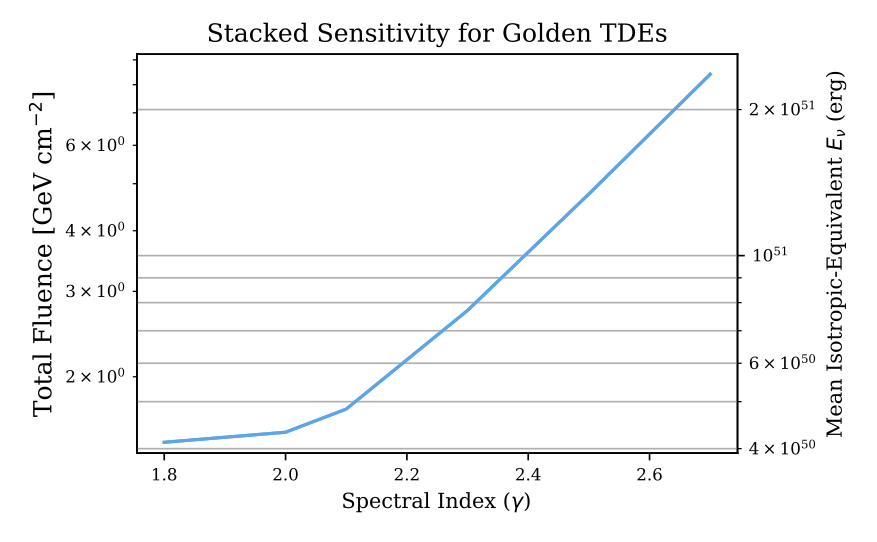
\includegraphics{results/gold_flux}
	\caption{Limits on the neutrino fluence and source energy for each catalogue. (Include numu + numubar in plot)}
	\label{fig:cat_upper_limit}
\end{figure}

\subsection{Population limits}

While the limits presented above constrain the contribution of those catalogues tested, we ultimately wish to constrain neutrino emission for the TDE population as a whole. If we \emph{assume that catalogue sources are representative of the broader population}, we can extrapolate from our per-source standard candle limits in Figure \ref{fig:cat_upper_limit} to the population flux. We seek to constrain the flux of two populations, namely jetted and non-jetted TDEs. For the latter case, we rely on the results of the golden TDE catalogue, since the extrapolation \emph{implicitly requires that the catalogues are not contaminated by misclassified objects}.

Using the most recent IceCube global fit of the astrophysical neutrino flux \sidecite{ic_global_fit_15}, with a best-fit spectrum of $E^{-2.50}$, we follow the procedure outline in Chapter \ref{ch:neutrino_cosmology}. We combine the golden TDE per-source limit shown in Figure \ref{fig:cat_upper_limit}, with a central local rate of $8 \times 10^{-7}$ Mpc$^{-3}$ year$^{-1}$ \sidecite{2018ApJ...852...72V} and a TDE source evolution derived by \cite{Sun:2015bda}. We constrain the contribution of non-jetted TDEs to be less than 26\% of the total. For jetted TDEs, under the assumption that they follow the same underlying source evolution as non-jetted TDEs with a central rate of $3 \times 10^{-11}$ Mpc$^{-3}$ year$^{-1}$ \sidecite{Sun:2015bda}, we find that they must contribute less than 1\% of the total.  These constraints are illustrated in Figure \ref{fig:DiffuseFlux}. 

\begin{figure}[!ht]
	\centering 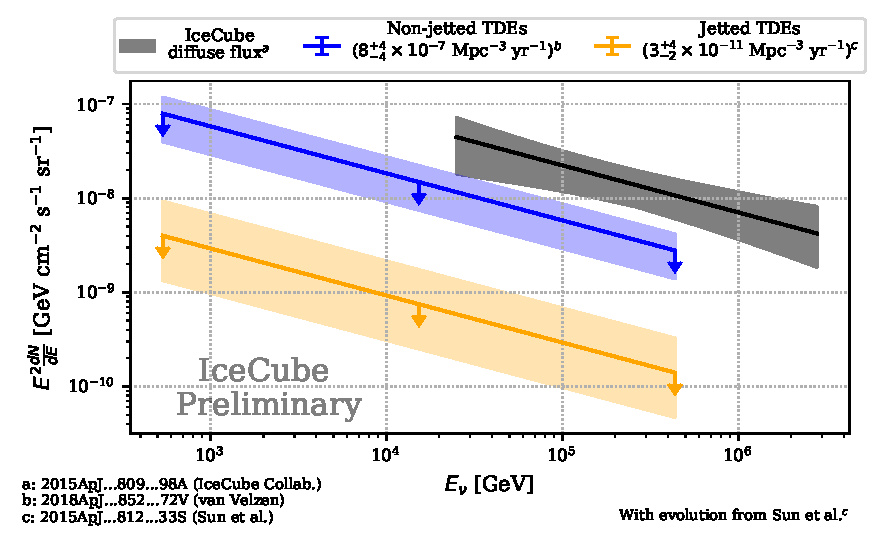
\includegraphics{results/tde_limits}
	\caption{Limits on the contribution of jetted and non-jetted TDEs to the diffuse neutrino flux.}
	\label{fig:DiffuseFlux}
\end{figure}

As the contribution from a population is directly proportional to the local population rate, the shaded bands indicate the uncertainty in our limits arising from rate estimates. For TDEs, these rates are the dominant source of uncertainty in neutrino flux. It will require systematic evaluation of observed TDE rates to enable more precise limits on neutrino emission. Any refined rate estimate can be used to linearly rescale these limits. Propagating through the current local rate uncertainty, we constrain non-jetted TDEs to be less than 13-39\%, and jetted TDEs to be less than 0.n-1.n\% of the total. With a more precise future measurement of the local TDE rate, these values can be linearly rescaled to provide more accurate limits.

Such limits also critically depend on the source evolution of TDEs as a function of redshift, but this is essentially unconstrained observationally because TDEs detections are overwhelmingly confined to the local universe (z $\lesssim$ 0.3). Estimates are made primarily based on theoretical predictions derived from the rate of SuperMassive Black Holes (SMBHs)?? \cite{Sun:2015bda}. If we instead consider a source evolution similar to the Star Formation Rate (SFR), as derived by CLASH-CANDELs, we would find limits of x and y \% respectively. For such a scenario, the contribution of unresolved TDEs is so large that the measured flux itself provides a stricter constraint than the catalogue test?

\subsection{Individual TDEs}

In addition, four TDEs were selected for individual analysis. Two of the three jetted TDEs, Swift J1644+57 and Swift J2058+05, were chosen due to their luminosity, as well as their position in the northern hemisphere where IceCube has the highest effective area. In addition, ASSASN-14li and  XMMSL1 J0740-85 were chosen as non-jetted TDEs which were both nearby and bright. These four TDEs were the only catalogue sources that were also detected in radio observations, typically a tracer for relativistic particle acceleration.

For each of the four individual TDEs, searches were conducted for neutrino clustering in both time and space, following the procedure outlined in Section \ref{sec:cluster_algorithm}. All single-object tests are described in Table \ref{tab:single_tests}

\begin{table*}[]
	\centering
	\begin{tabular}{||c |c c c c | c c c c| c||} 
	\hline
	Source & R.A & Dec & T$_{0}$ & T$_{1}$ & n$_{s}$ & $\gamma$ & t$_{s}$ & t$_{e}$ & TS\\
	& (deg.) & (deg.) & (MJD) & (MJD) & & & (MJD) & (MJD) & \\
	\hline
	Swift J1644+57 & 251.21 & 57.58 & 55644.00 & 55749.00 & 0.68 & 1.98 & 55650.90 & 55746.25 & 0.06\\
	Swift J2058+05 & 314.58 & 5.23 & 55694.00 & 55798.00 & 2.78 & 4.00 & 55774.25 & 55780.00 & 2.28\\
	ASASSN-14li & 192.06 & 17.77 & 56851.00 & 57072.00 & 2.95 & 2.53 & 57022.68 & 57032.75 & 1.52\\
	XMMSL1 J0740-85 & 115.03 & 85.66 & 56718.00 & 56848.00 & 2.84 & 2.19 & 56806.95 & 56807.51 & 3.49\\
	\hline
	AT2018cow & 244.00 & 22.27 & 58256.90 & 58386.90 & 5.91 & 2.98 & 58283.83 & 58298.53 & 3.91\\
	\hline
	\end{tabular}
	\caption{Summary of the five individual TDEs for which the temporal-cluster-search method was applied. All but AT2018cow were included in the stacking analysis.}
	\label{tab:single_tests}
\end{table*}{}

The results of each fit are provided in Table N, alongside pre-trial p-values. No significant emission was identified, and no discovery is claimed. Instead, upper limits are derived on neutrino emission for each source. As described in Section \ref{sec:cluster_algorithm}, the cluster-search method is more sensitive to shorter-scale emission. Upper limits were derived under the conservative assumption that neutrino emission was distributed uniformly in the search window, with any emission on shorter timescales being more constrained. 

\section{AT2018cow and FBOTs}

Following the four stacking analyses and four object analyses described above, an additional analysis was performed on AT2018cow \sidecite{Margutti:2018rri}. This object was a fast, bright, blue transient first discovered in 2018. The observations suggested AT2018cow was a nearby example of a recently-identified population of Fast Blue Optical Transients (FBOTs) \sidecite{drout_fbot}. 

At the time of discovery, AT2018cow was initially thought to be a bright Broad-Lined type Ic (Ic-BL) supernova, and thus a member of the rare subclass associated with long GRBs and relativistic jets \sidecite{sn_grb_06}. As outlined in Chapter \ref{ch:sources}, many models predict that such SNe may be neutrino sources, so an IceCube \emph{Fast Response Analysis} was run on AT2018cow shortly after discovery \sidecite{icrc_fra}. The IceCube search targeted choked-jet neutrino emission, and thus covered the 3-day period from the last non-detection to the first detection, aiming to isolate the supernova explosion time at which the neutrino emission would be expected. Ultimately, an excess of neutrinos was found in this time period, with a significance of 1.8 $\sigma$ \sidecite{2018ATel11785....1B}. The excess itself consisted of two signal-like neutrinos, which were considered significant owing to the small expected background for such a short search window.

Later multi-wavelength observations of AT2018cow were not consistent with a traditional Ic-BL SN, and the transient was instead identified as a nearby example of an FBOT \sidecite{Perley:2018oky}. The exact nature of these FBOTs had been difficult to probe, since they were primarily discovered at high redshift \cite{drout_fbot}, but promptly-identified AT2018cow at 60 Mpc provided a rich multi-wavelength dataset. It has since variously interpreted as a TDE with an Intermediate-Mass Black Hole, an extreme supernova or a Magnetar . In light of these developments, AT2018cow was re-analysed by the author in the context of a potential TDE classification. As for the other four individual TDEs detailed above, a dedicated search for neutrino clustering on timescales up to 130 days, extending from 30 days before peak to 100 days afterwards, was undertaken.  For this purpose, an additional year of IceCube data extending to October 2018 was analysed.

In this analysis of AT2018cow, a small excess was again found. Although the best-fit cluster from this search included the two signal-like neutrinos from the original IceCube analysis, when accounting for the expected fluctuations arising from background over the much longer 130 day search window, the significance of the excess was just 0.5 $\sigma$. The result is thus entirely consistent with expectations from atmospheric background, while not contradicting the original result published at the time. As such, no discovery is claimed and upper limits are accordingly derived (illustrated in Figure \ref{fig:at2018cow_limits}). Though AT2018cow was not included in the catalogues when the stacking analysis was performed, it would naturally belong to the silver non-jetted TDE sample. 

\begin{figure}[!ht]
	\centering 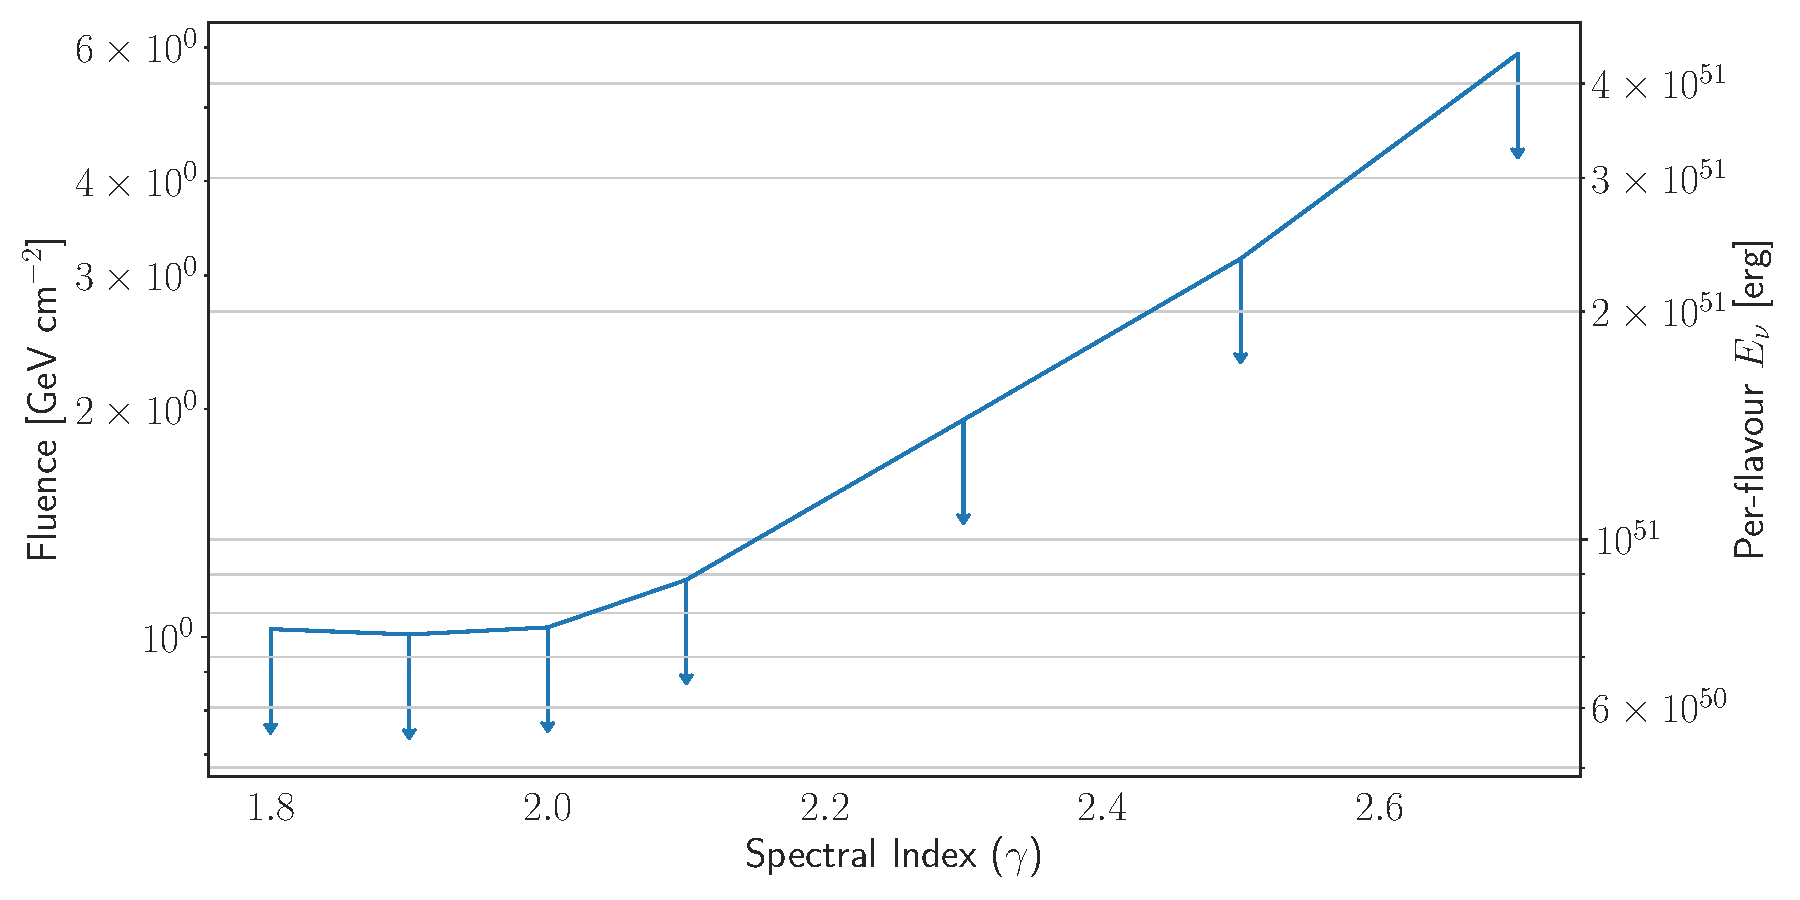
\includegraphics{results/at2018cow_limits}
	\caption{Limits on neutrino emission from AT2018cow, as a function of spectral index.}
	\label{fig:at2018cow_limits}
\end{figure}

The analysis of AT2018cow is the first example of a test for neutrino emission from FBOTs. In the two years since discovery in 2018, there have been theoretical studies considering possible neutrino emission from FBOTs in general, and AT2018cow in particular \sidecite{fang_fbot}. The predicted neutrino emission is typically several orders of magnitude below the limits presented in Figure \ref{fig:at2018cow_limits}, as shown in Figure N, and thus further supports the likely atmospheric origin for the neutrino excess \cite{2018ATel11785....1B}.

Given that AT2018cow is by far the closest example of an FBOT, we can already consider the implications for the broader population emission, following the same procedure above. While initial estimates suggested that these objects might equal $\sim$4-7\% of the CCSN rate \cite{drout_fbot, fang_fbot}, the lack of additional FBOTs in recent magnitude-limited surveys such as ZTF strongly suggest that the local rate to be $<$ 1.0\% of the CCSN rate \sidecite{ho_koala}, CITE ZTF BTS. This has implications for previous work. 

Following the same procedure for TDEs, we find that FBOTs contribute less than 16\% of the total diffuse neutrino flux \emph{assuming that AT2018cow is representative of the broader FBOT population}. This further assumes a CCSN-like source evolution \sidecite{sfr_madau_14}, proportional to the star formation rate, and a local FBOT rate of 4 $\times$ 10$^{-7}$ Mpc$^{-3}$ yr$^{-1}$ \cite{ho_koala}.

\begin{figure}[!ht]
	\centering 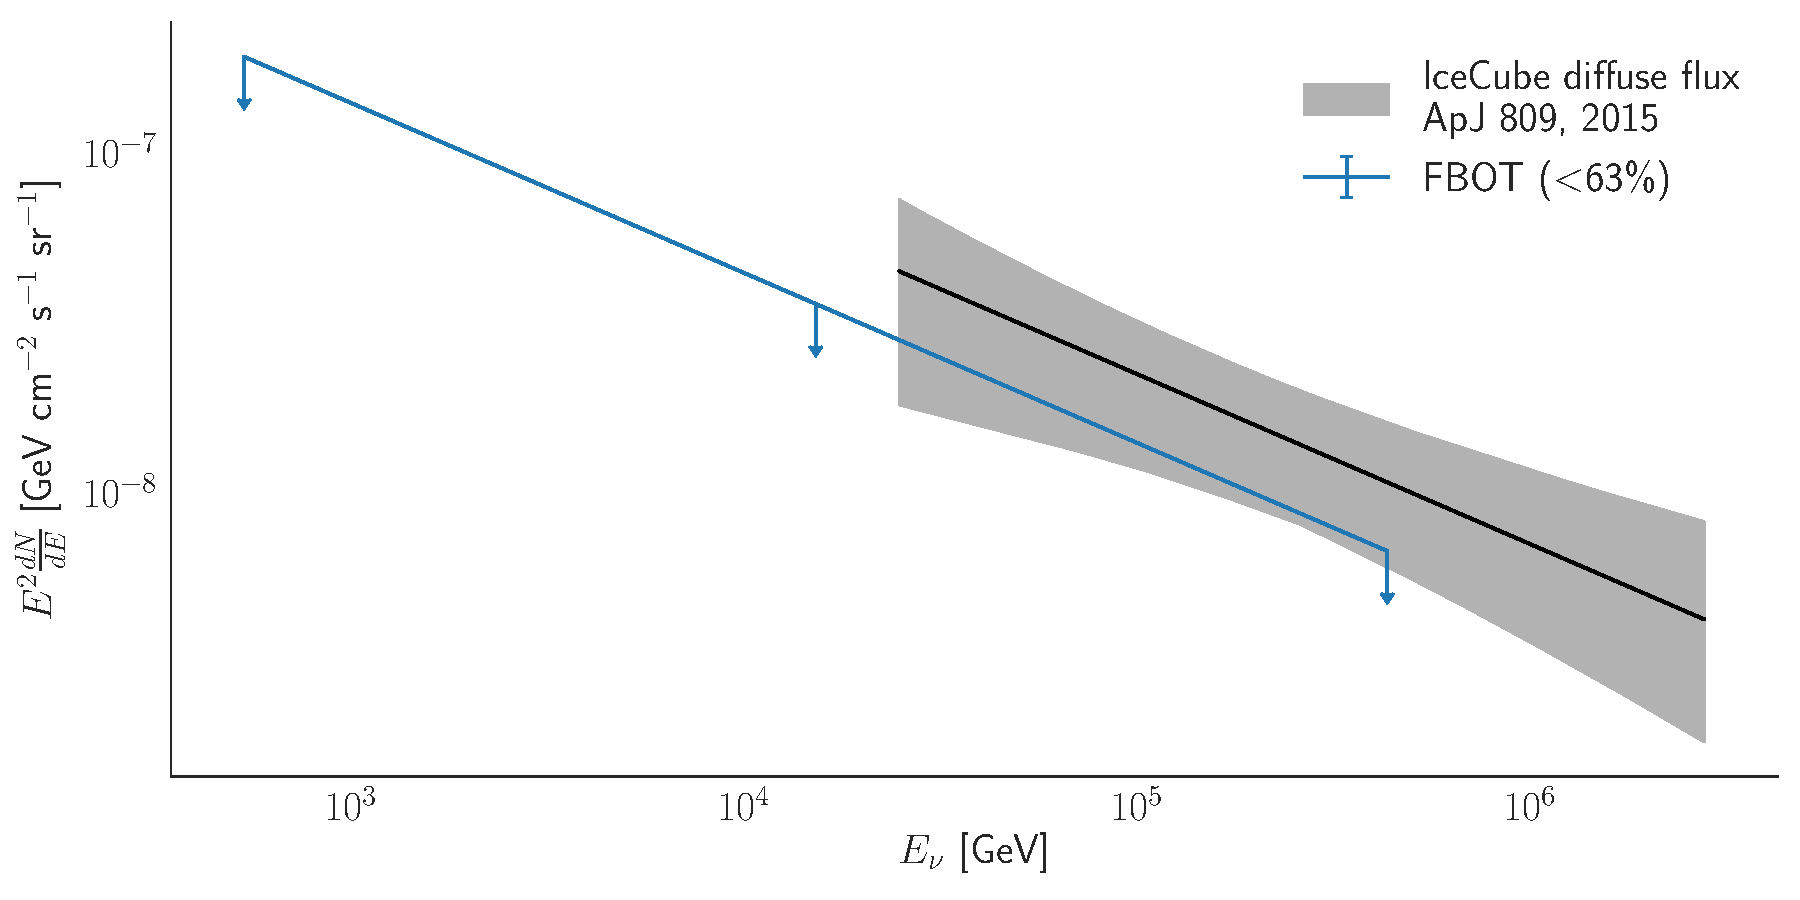
\includegraphics{results/fbot_limits}
	\caption{Limits on neutrino emission from FBOTs, using the limits from AT2018cow under the assumption of neutrino standard candles.}
	\label{fig:fbot_limits}
\end{figure}

Systematics 10\%
\setchapterimage[6.5cm]{Grid_FullView_Logo}
\setchapterpreamble[u]{\margintoc}
\chapter{Realtime Multi-Messenger Astronomy}
\labch{realtime}
\begin{fquote}[Isaac Asimov][Lady Windermere's Fan][18??] A stopped clock is right twice a day.
\end{fquote}

In recent years, there has been a significant renewed interest in the study of transient and variable objects in astronomy. Driven primarily by the speed at which objects can evolve and disappear, particularly GRBs and latterly Kilonovae, it is often essential that astronomy can be done with minimal latency. In this vein, it is now commonplace for detectors to automatically issue so-called alerts for observations that meet given criteria, to enable other instruments to rapidly obtain near-simultaneous observations. Realtime alerts are automatically issued by GRB-searching instruments such as Swift-BAT and Fermi-GBM, while gravitaional-wave events are issued by the LIGO-VIRGO observatories, and high-energy neutrino alerts are issued by IceCube as well as ANTARES.

These alerts are all typically issued via  the Gamma-ray Coordination Network (GCN) system, where observatories can subscribe to automatically be notified or point.  An essential component of this process is the additional information published by astronomers, via GCN or Astronomers Telegrams (ATELs), in which follow-up observations are coordinated. There have been two high-profile examples of this, namely the comprehensive followup of GW170817/GRB170817A that led to the first unambiguous observation of a kilonovae, and the followup of high-energy neutrino IC170922A, which led to the identification of TXS 0506+056 as the first candidate source of TeV neutrinos. 

As part of this thesis, the author maintained and further developed the IceCube Realtime System from October 2018 onwards, acting as first responder to the vast majority of neutrino alerts in that period.

\section{The IceCube Realtime System}
The IceCube Realtime System has been operating since 2016, providing the first source of high-energy neutrino alerts. The first iteration of the alert system consisted of two streams, namely High-Energy Starting Events (HESE) and Extremely High Energy (EHE) events CITE. Each was an established event selection used to identify likely-astrophysical neutrinos cite. Filters to identify relevant events are deployed on computers at the South Pole, and detections are flagged  with low latency. After fast "online" reconstruction algorithms are applied to events, an automated machine-readable "notice" is distributed via the GCN system. In parallel, data from the event is transmitted via satellite to a computing centre in Madison, Wisconsin where a full likelihood scan is performed on the event (see chapter \ref{ch:Event Selection and Reconstruction} for more details). 

Give V1 rates!

The alerts are vetted by humans to asses the event quality, with visually inspection being used to confirm classified topology and event reconstructions. The operating state of the detector is additionally checked. Following these steps, a plain-text GCN circular is distrubuted via the GCN system to confirm the good nature of the alert, and to provide the updated localisation arising from the full scan. 

This original system of alerts continued until May 2019, at which point a new alert system was implemented. While the original EHE selection was maintained, the HESE alert selection was improved to reduce the cascade contamination, and improve the astrophysical purity. In addition, a new alert stream based on the GFU event selection was initiated, with a significantly-elevated rate relative to EHE and HESE alerts. The publication of these three alert streams was unified into a new IceCube Astrotrack GCN stream, which was further subdivided into Gold and Bronze based on the average purity of alerts. Golden Astrotrack alerts will, as an ensemble, have an average of 50\% astrophysical neutrinos, while Bronze Astrotrack will have an average of 30\% astrophysical neutrinos.

A summary of all neutrino alerts issued to date is provided in table X. Individual neutrino alerts of interest are summarised in subsequent sections. 

\subsection{IC160427A - The "PanSTARRS Supernova Neutrino"}

The first alert issued under this system, HESE alert IC160427A, was found to be in spatial coincidence with an optical transient detected by the Pan-STARRS Observatory while following up the alert. This transient was initially tentaively classified as a Type Ic supernova, for which various models have predicted neutrino emission (see Chapter \ref{ch:sources}).  However, the further spectroscopic and photometric evolution indicated that this was  more likely a Type Ia Supernova, for which no neutrino emission would be expected. Nonetheless, dedicated efforts to simulate an ensemble of IC160427A-like events led to the first characterisation of the impact of systematic uncertainties in modelling the polar glacial ice on directional reconstruction with IceCube for high-energy alerts. 

\subsection{IC170922A The "TXS 0506+056 Neutrino"}
Subsequent neutrino alerts did not yield any probable counterparts, until the detection of EHE alert IC170922A in spatial coincidence with flaring blazar TXS 0506+056. Chance coincidence in this case was estimated  This event was also resimulated in the same manner as IC160427A. Remarkably, despite its radically-different topology of through-going muon rather than starting track, the results were found to be broadly consistent. More details are given in chapter N.

\subsection{IC190331A - The "Multi-PEV Neutrino"}

A starting track was observed 

\subsection{IC190730A - The "ICRC Neutrino"}

IC190730A was a golden neutrino alert with a signalness of roughly 65\%. Following the automated notice, Millipede Reconstruction clearly showed it was well-localised, and spatially coincident with blazar PKS 1502+106. This particular blazar is extremely bright, being Nth brightest in the sky in terms of integrated gamma-ray energy flux, and owing to its high redshift of z=1.84, is one of the most luminous known blazars. This coincidence was reported in the corresponding GCN circular, and triggered a broad multi-wavelength follow-up campaign. The archival SED is provided in figure N, originally from X, but annotated to illustrate contemporaneous observations from other instruments.

\begin{figure}[!ht]
	\centering 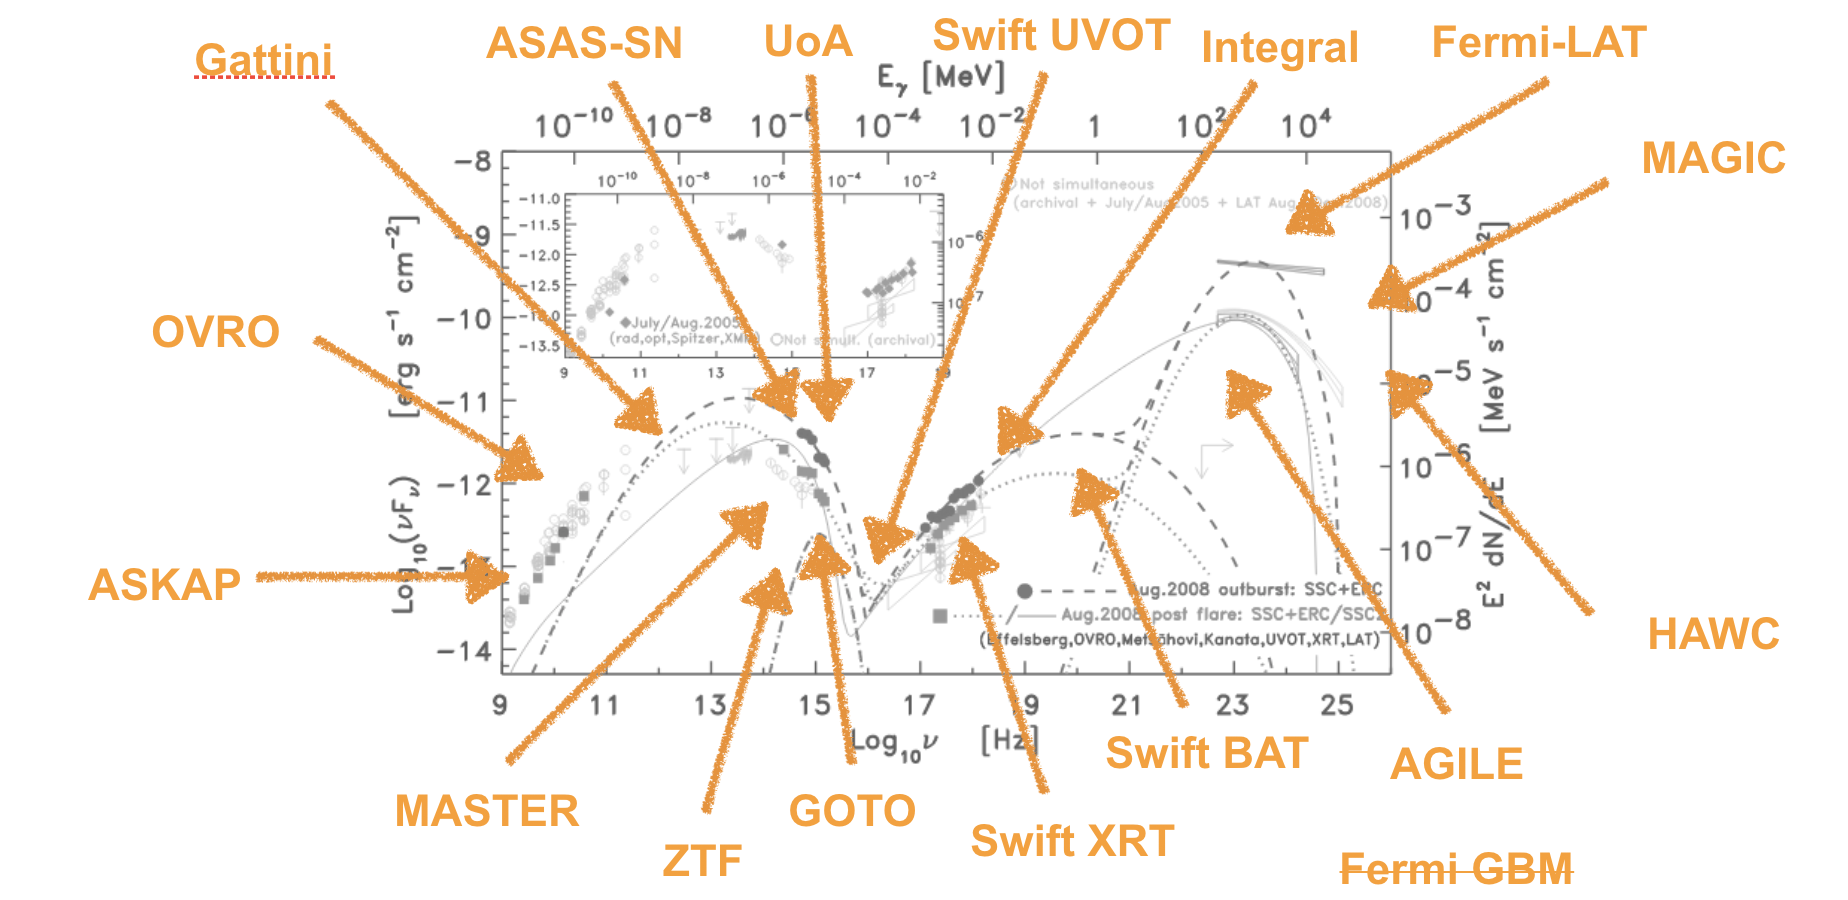
\includegraphics{pks_followup}
	\caption{The archival SED of PKS 1502+106 from X is shown. In orange, the names of various instruments that observed the source are overlaid, with orange arrows to indicate their corresponding energy regimes. CITEA-Z}
	\label{fig:PKSobs}
\end{figure}

Despite comprehensive wavelength coverage, 

The chance coincidence for at least one neutrino alert to be coincident with any of the  15 brightest blazars was calculated by the author, and found to be disfavoured at the level of 2.n sigma following the procedure in N. 

\subsection{IC190922B - The "SN2019pqh Neutrino"}

\subsection{IC191001A - The "Bran Stark Neutrino"}

\subsection{IC200107A - The "Flaring Extreme Blazar neutrino"}

\section{Interpreting high-energy neutrino alerts}

lalala

\subsection{Cluster searches}
lalaland

\subsection{OFU and GFU}.
\setchapterimage[7.5cm]{palomar}
\setchapterpreamble[u]{\margintoc}
\chapter{Transient Follow-up with ZTF}
\labch{ztf_too}
\begin{fquote}[Oscar Wilde][Lady Windermere's Fan][18??]We are all in the gutter, but some of us are looking at the stars
\end{fquote}

The motivation for all real-time analysis and prompt follow-up observations of external triggers is to obtain contemporaneous data. Put another way, these observations are designed to quickly identify time-dependent transient or variable activity which would be missed by untargeted survey operations.  In the case of GW and short GRB follow-up, searches are targeted towards identifying kilonovae (KNe), of which GW170817/AT2017gfo was a spectacular well-documented first example. These KNe are inherently fast-evolving transients which will by definition not be present before the extrenal trigger. For neutrinos, there are a proliferation of possible optical transients (e.g GRBs, TDEs, SNe) and variable objects (primarily blazars) which could be identified in an optical follow-up observations. In both cases, a handful of potentially interesting extragalactic objects will need to be selected against a vast background of spurious detections, and unrelated galactic or solar-system objects.

\section{The AMPEL Follow-up Pipeline}
Given the similar challenge, a single flexible analysis, the \ztf, was developed by the author to identify candidate counterparts to GW, GRB and neutrino trigger events. ZTF is particularly well-suited to this type of extragalactic transient discovery,  because ZTF routinely images the visible Northern Sky once every three nights to a median depth of $20.5^{m}$ as part of a public survey \sidecite{2019PASP..131g8001G, 2019PASP..131a8002B}.  This provides an extensive base to distinguish between new transients that could be coincident with an external trigger, and those with previous detections. The large volumetric survey speed of ZTF often provides significant serendipitous coverage of events. This wide-field cadence can however be supplemented by dedicated Target-of-Opportunity (ToO) observations scheduled for a particular trigger through the GROWTH ToO Marshal \sidecite{2019PASP..131d8001C}. 

Following both survey and ToO observations, the raw images are processed by IPAC, and alert packets are promptly generated for significant differences relative to survey reference images \sidecite{2019PASP..131a8003M,2019PASP..131a8001P}. These alerts are then distributed as part of a near-realtime stream to brokers, and are archived in a database of alert packets at DESY as part of the local infrastructure for multi-messenger data analysis (the \emph{archive database}).

External triggers, which come in the form of probability skymaps or GCN circulars, are downloaded and parsed with \ztf. The archive database is then queried for coincident alerts, using either temporal indexing or spatial indexing depending on the size of the target region. Once loaded, these alerts are then filtered by the \ztf~using \emph{AMPEL} \sidecite{2019A&A...631A.147N}, a platform for realtime analysis of multi-messenger astronomy data. Our selection is based on an algorithm for identifying extragalactic transients \cite{2019A&A...631A.147N}. In order to identify candidate counterparts, we apply the following cuts to ToO and survey data:

\begin{itemize}
	\item We reject likely subtraction artifacts using machine learning classification and morphology cuts \sidecite{2019PASP..131c8002M}. Subtractions must be positive, i.e a candidate must be brighter than the same position in stacked reference images.
	\item We reject solar system objects through matches to known catalogues \cite{2019PASP..131a8003M}. We further remove uncatalogued solar system objects by requiring multiple detections for each candidate at the same location, separated temporally by at least 15 minutes, thereby rejecting moving objects.
	\item We reject galactic stellar sources by removing detections cross-matched to objects with measured parallax in the second data release of the \emph{GAIA} satellite \sidecite{2018A&A...616A...1G}. Objects are rejected if they have non-zero parallax with a significance of at least 3$\sigma$. We further reject likely stars with machine learning classifications, based on sources detected by Pan-STARRS1 \sidecite{2018PASP..130l8001T}, removing those objects with an estimated stellar probability greater than 80\%. 
	\item We reject AGN variability by cross-matching objects to the WISE survey. We identify likely AGN by applying a series of cuts based on measured IR colour \sidecite{2010AJ....140.1868W}.
	\item We rejected unassociated objects by requiring both spatial and temporal coincidence with a given trigger.
\end{itemize}

\section{Neutrino Follow-up}
ZTF has since its inception had a dedicated program to identify sources of high-energy astrophysical neutrinos, through targeted follow-up observations. Given the proliferation of proposed source classes, neutrino follow-up are characterised by searching relatively well-localised regions for poorly-defined objects. This is particularly true for optical follow-up, where potential counterparts include Tidal Disruption Events (TDEs), Type IIn or choked jet SNe, kilonovae, GRB afterglows, superluminous supernovae (SLSNe) or blazar flares. While pre-neutrino detections could rule out neutrino production from choked jet supernovae, in most cases we do not even have stringent constraints in when neutrinos may be expected 

 We have followed up eight neutrinos in the period from survey start on 2018 March 20 to 2020 March 31, out of a total of 31 neutrino alerts published by IceCube. Table \ref{tab:nu_alerts} summarises each neutrino alert that has been observed by ZTF. From 2019 June 17, IceCube published neutrino alerts with improved selection criteria to provide an elevated alert rate \sidecite{2019ICRC...36.1021B} (see Chapter \ref{ch:realtime} for more details). In addition to 1 of the 12 alerts under the old V1 selection, ZTF followed up 7 of the 19 alerts published under the V2 selection. In general, we aim to follow all well-localised neutrinos of likely astrophysical origin reported by IceCube which are visible to ZTF and can be observed promptly. Those alerts not observed by ZTF are summarised in Table \ref{tab:nu_non_observed}. Of those 23 alerts not followed up by ZTF, the primary reasons were proximity to the Sun (8/23), alerts with poor localisation and low astrophysical probability (6/23) and alert retraction (4/23). For events which were reported with estimates of astrophysical probability\footnote{This value was not reported for high-energy starting events (HESE) under the old IceCube alert selection, nor for one recent alert, IC200107A, that was identified outside of the standard alert criteria \sidecite{stein:gcn26655}.}, we chose not to follow up those that had both low astrophysical probability ($<$ 50\%) and large localisation regions ($>$ 10 sq.\,deg.).

\begin{table*}
	\centering
	\begin{tabular}{||c c c c c c c ||} 
		\hline
		\textbf{Event} & \textbf{R.A. (J2000)} & \textbf{Dec (J2000)} & \textbf{90\% area} & \textbf{ZTF obs} &~ \textbf{Signalness}& \textbf{Ref}\\
		& \textbf{(deg)}&\textbf{(deg)}& \textbf{(sq. deg.)}& \textbf{(sq. deg.)} &&\\
		\hline
		IC190503A & 120.28 & +6.35 & 1.94& 1.37 & 36\%&\cite{blaufuss:gcn24378,2019ATel12730....1S}\\
		IC190619A & 343.26 & +10.73 & 27.16& 21.57 & 55\%&\cite{blaufuss:gcn24910, 2019ATel12879....1S}\\
		IC190730A & 225.79 & +10.47 & 5.41& 4.52 & 67\%&\cite{stein:gcn25225, 2019ATel12967....1T, 2019ATel12974....1S}\\
		IC190922B & 5.76 & -1.57 & 4.48 & 4.09 & 51\%&\cite{blaufuss:gcn25806,2019ATel13125....1S, stein:gcn25824}\\
		IC191001A & 314.08 & +12.94 & 25.53 & 20.56 & 59\%& \cite{stein:gcn25913,2019ATel13160....1S, stein:gcn25929}\\
		IC200107A\footnote{This event was reported without a signalness estimate} & 148.18 & +35.46 & 7.62 & 6.22 & - &\cite{stein:gcn26655,stein:gcn26667}\\
		IC200109A & 164.49 & +11.87 & 22.52 & 20.06 & 77\%&\cite{stein:gcn26696,reusch:gcn26747}\\
		IC200117A & 116.24 & +29.14 & 2.86 &  2.66 & 38\%&\cite{lagunas:gcn26802,reusch:gcn26813, reusch:gcn26816}\\
		IC200512A\footnote{This event occurred at low galactic latitude, and thus our observations were not sensitive to extragalactic objects.}&295.18&+15.79&9.77&9.67&32\%&\cite{IC200512A}\\
		IC200530A&255.37&+26.61&25.28&22.75&59\%&\cite{IC200530A}\\
		IC200620A&162.11&+11.95&1.73&1.34&32\%&\cite{IC200620A, ztf_IC200620A}\\
		\hline
	\end{tabular}
	\caption{Summary of the eleven neutrino alerts followed up by ZTF. The 90\% area column indicates the region of sky observed at least twice by ZTF, within the reported 90\% localisation, and accounting for chip gaps. The \textit{signalness} describes the probability that each neutrino is of astrophysical origin, rather than arising from atmospheric backgrounds.}
	\label{tab:nu_alerts}
\end{table*}

\begin{table}
	\centering
	\begin{tabular}{||c c||} 
		\hline
		\textbf{Cause} & \textbf{Events} \\
		\hline
		\textbf{Alert Retraction} & IC180423A\cite{IC180423A}, IC181031A\cite{IC181031A},\\ &IC190205A\cite{IC190205A}, IC190529A\cite{IC190529A}\\
		&\\
		\hline
		\textbf{Proximity to Sun} & IC180908A\cite{IC180908A}, IC181014A\cite{IC181014A},\\ &IC190124A\cite{IC190124A}, IC190704A\cite{IC190704A},\\
		& IC190712A\cite{IC190712A}, IC190819A\cite{IC190819A},\\
		& IC191119A\cite{IC191119A}, IC200227A\cite{IC200227A}\\
		&\\
		\textbf{Low Altitude} & IC191215A\cite{IC191215A}, IC200615A\cite{IC200615A}\\
		&\\
		\textbf{Southern Sky} & IC190331A\cite{IC190331A}, IC190504A\cite{IC190504A}\\
		&\\
		\hline
		\textbf{Poor Signalness \& Localisation} &
		IC190221A\cite{IC190221A}, IC190629A\cite{IC190629A}, \\
		&IC190922A\cite{IC190922A}, IC191122A\cite{IC191122A}, \\
		&IC191204A\cite{IC191204A}, IC191231A\cite{IC191231A}\\
		&IC200410A\cite{IC200410A}, IC200421A\cite{IC200421A}\\
		& IC200425A\cite{IC200425A}, IC200523A\cite{IC200523A}\\
		&IC200614A\cite{IC200614A}\\
		&\\
		\hline
		\textbf{Bad Weather} & IC200120A\cite{IC200120A,IC200120A_2}\\
		&\\
		\textbf{Telescope Maintenance} & IC181023A\cite{IC181023A}\\
		&\\
		\hline
	\end{tabular}
	\caption{Summary of the 23 neutrino alerts that were not followed up by ZTF since survey start on 2018 March 20. Of these, 4/23 were retracted, 11/23 were inaccessible to ZTF for various reasons, 6/23 were deemed alerts of poor quality, while just 2/23 were alerts that were missed although they passed our criteria.}
	\label{tab:nu_non_observed}
\end{table}

Each neutrino localisation region can typically be covered by one or two ZTF observation fields. Multiple observations are scheduled for each field, with both $g$ and $r$ filters, and a separation of at least 15 minutes between images. These observations typically last for 300~s, with a typical limiting magnitude of $21.0^{m}$.  ToO observations are typically conducted on the first two nights following a neutrino alert, before swapping to serendipitous coverage as part of the public survey. We search ZTF data both preceding and following the arrival of the neutrino. Our coincidence criteria require that an object lie within the 90\% localisation region reported by IceCube in a GCN circular, and must have been detected at least once following the neutrino arrival time. These cuts typically yield $\sim$0.2 candidates per square degree of sky. Promising candidates are prioritised for spectroscopic classification, to confirm or rule out a possible association with a given neutrino. 

A selection of highlighted  results are given below. A further candidate, AT2019dsg, is described in Chapter \ref{ch:bran}.

\subsection{PKS 1502+106}
As introduced in Chapter \ref{ch:realtime}, the neutrino IC190730A was reported in spatial coincidence with PKS 1502+106, a particularly bright Flat Spectrum Radio Quasar (FSRQ) \sidecite{2019ATel12967....1T}. The object was observed by ZTF as part of ToO observations, and the object DID was also identified by our follow-up pipeline as a candidate counterpart.  The blazar was repeatedly detected as part of the routine survey operations under the name \emph{ZTF18aaqnqzx}, with both positive and negative flux changes relative to survey reference images. The blazar lightcurve is shown in Figure \ref{fig:pks1502_ligtcurve}, with the neutrino arrival time marked in blue. Consistent with observations from other observatories across many wavelengths (Chapter \ref{ch:realtime}), there was no significant flaring observed for this source coincident with the neutrino. The blazar at this point was dimmer than survey reference images, with the neutrino arriving during a year-long fading. 

\begin{figure}[!ht]
	\centering 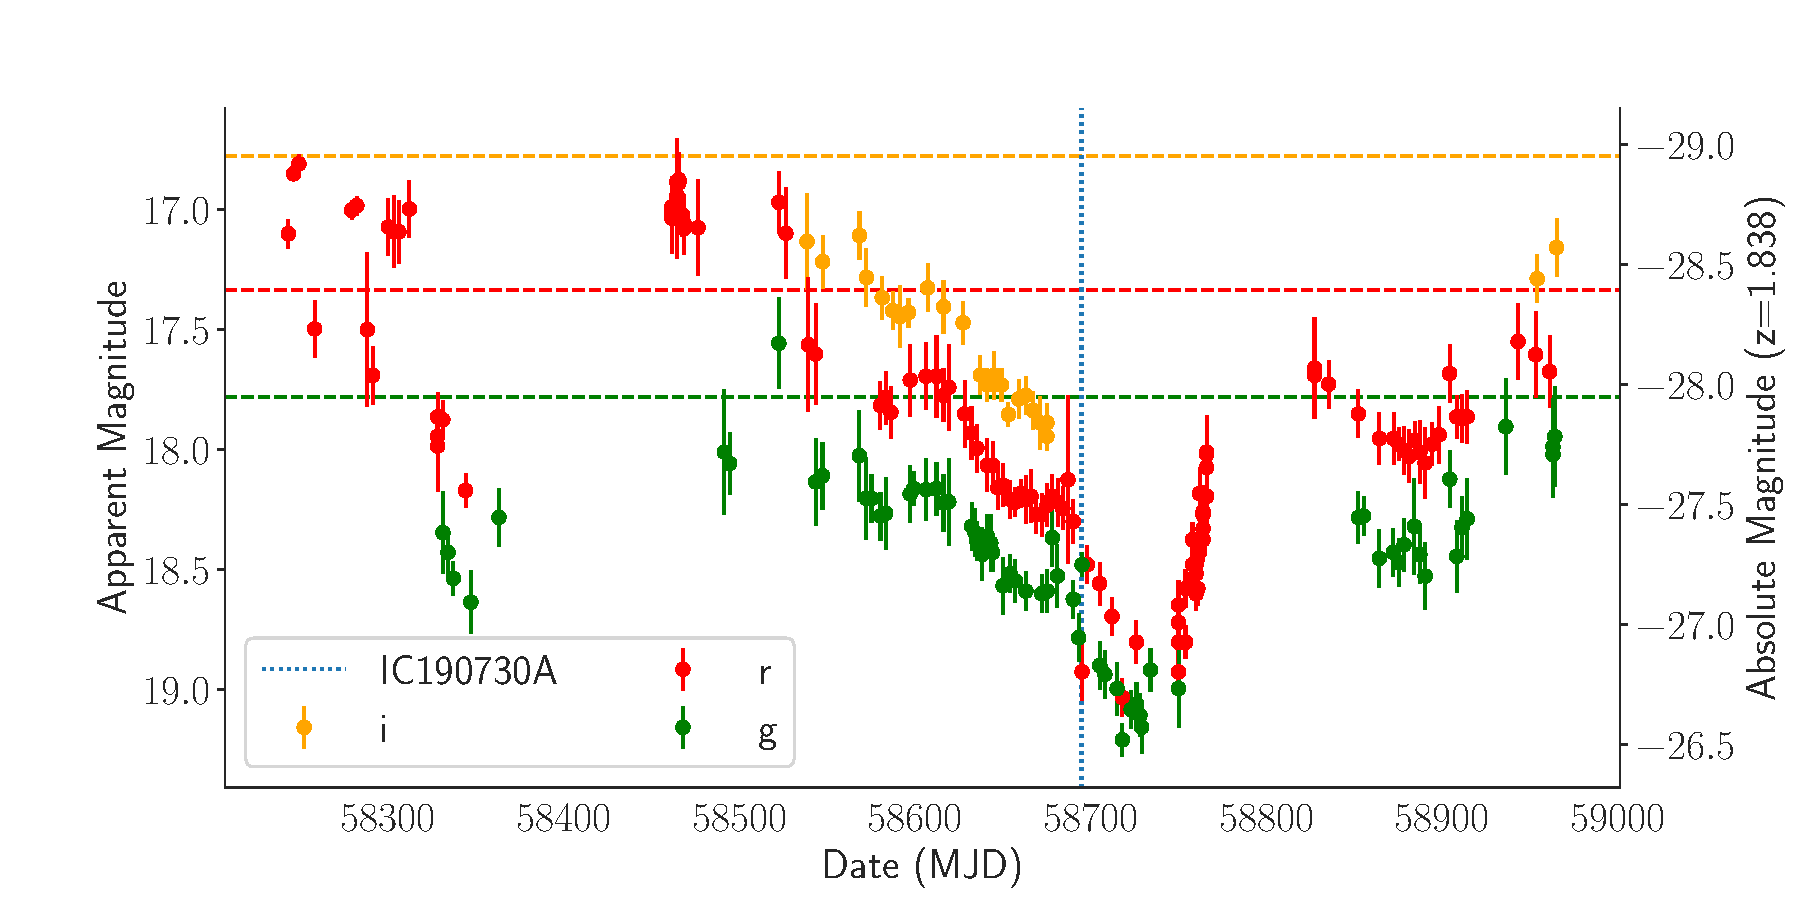
\includegraphics{ZTF/pks1502_lightcurve}
	\caption{ZTF lightcurve of blazar PKS 1502+106, with observations in g, r and i bands. The arrival time of the neutrino on 2019 July 30 is marked with a dotted line. The horizontal dashed lines indicate the magnitude of the source in reference images derived from the PanSTARRS survey.}
	\label{fig:pks1502_ligtcurve}
\end{figure}

\subsection{SN2019pqh}
As introduced in Chapter \ref{ch:realtime}, follow-up of IC190922B by ZTF identified a candidate supernova ZTF19abxtupj/SN2019pqh \sidecite{2019ATel13125....1S}. As outlined in chapter \ref{ch:sources}, neutrino emission has been predicted for core-collapse supernovae from either choked jets or interacting supernovae. SN2019pqh was not consistent with the former scenario, because it was detected prior to the neutrino. However, it was close to peak, as shown in the lightcurve in Figure \ref{fig:sn2019pqh_ligtcurve}. This was the first young supernova found in coincidence with a high-energy neutrino, which is interesting because CSM neutrino emission . 

\begin{figure}[!ht]
	\centering 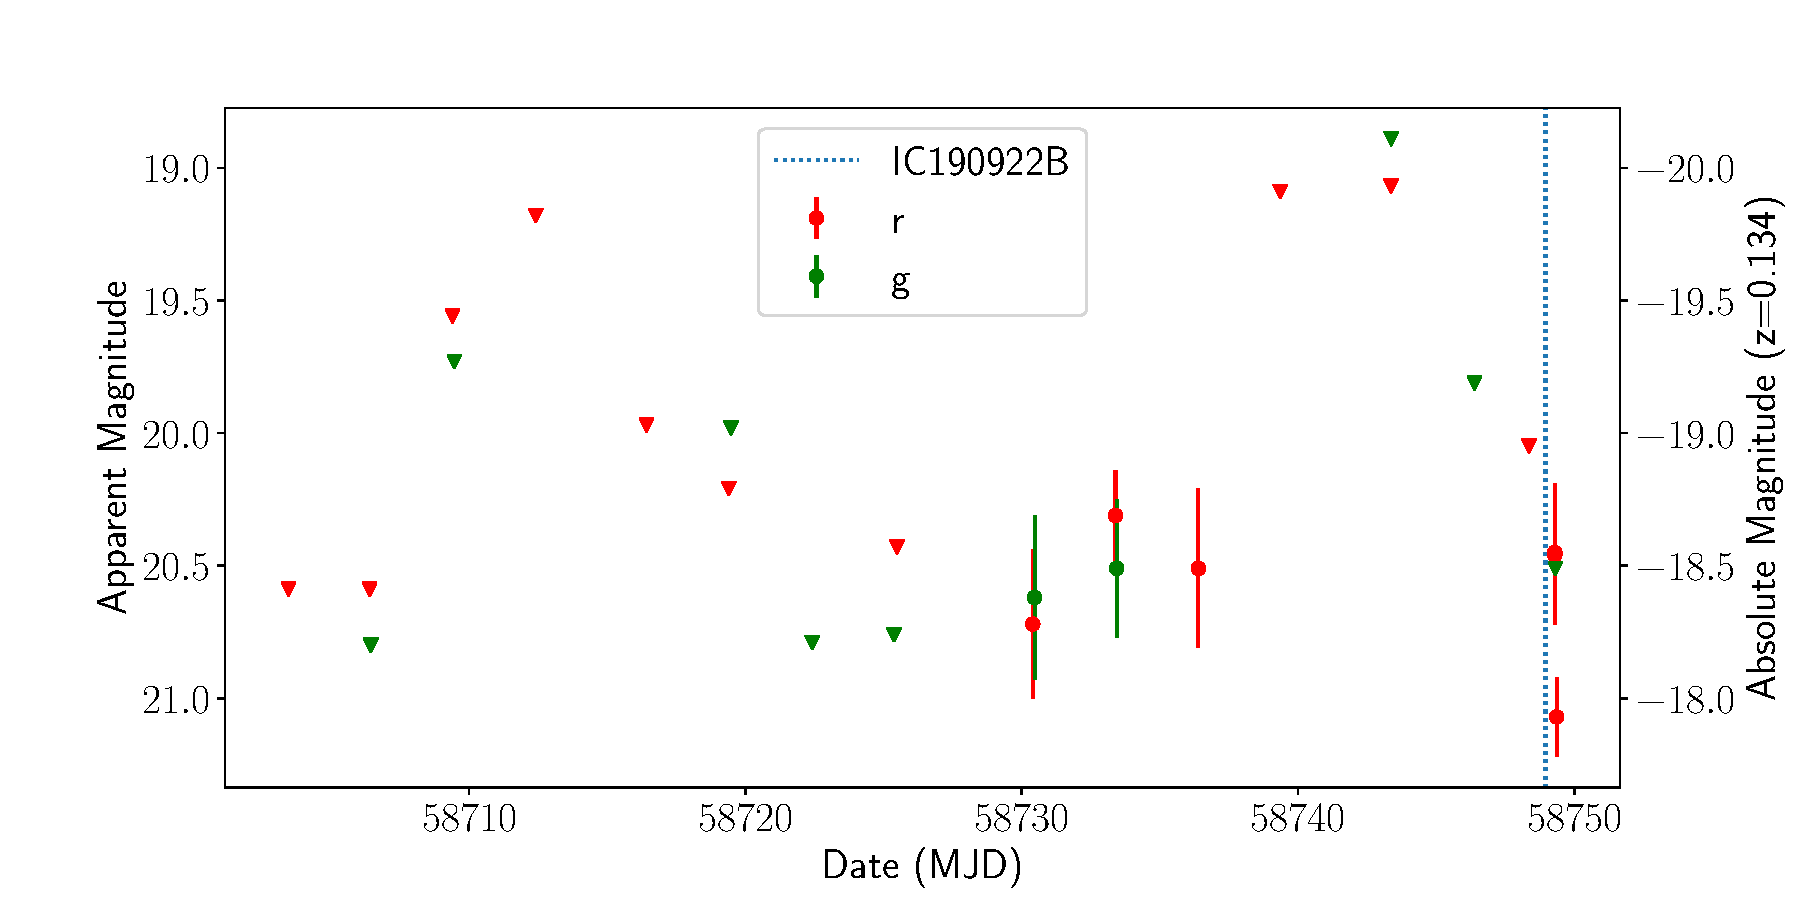
\includegraphics{ZTF/sn2019pqh_lightcurve}
	\caption{ZTF lightcurve of SN2019pqh, with observations in g and r band. The arrival time of the neutrino on 2019 September 22 is marked with a dotted line, and the supernova is detected in the subsequent ToO obsersations.}
	\label{fig:sn2019pqh_ligtcurve}
\end{figure}

This object had first been detected on A subsequent classification of the object as a Type II supernova was reported by ePESSTO (cite). 

A high-resolution spectrum of the object was obtained by De Sharma on 2019 September 28, using the (LRIS) spectrograph at the Keck 1 observatory (see Figure \ref{fig:sn2019pqh_spectrum}). The host galaxy, clearly visible in Figure N, had a spectroscopic redshift of z=0.134 measured by the Sloan .... (SDSS). Peaks are clearly visible in the spectrum matching hydrogen lines for this redshift, confirming that the transient is indeed coincident with the apparent host galaxy.

\begin{figure}[!ht]
	\centering 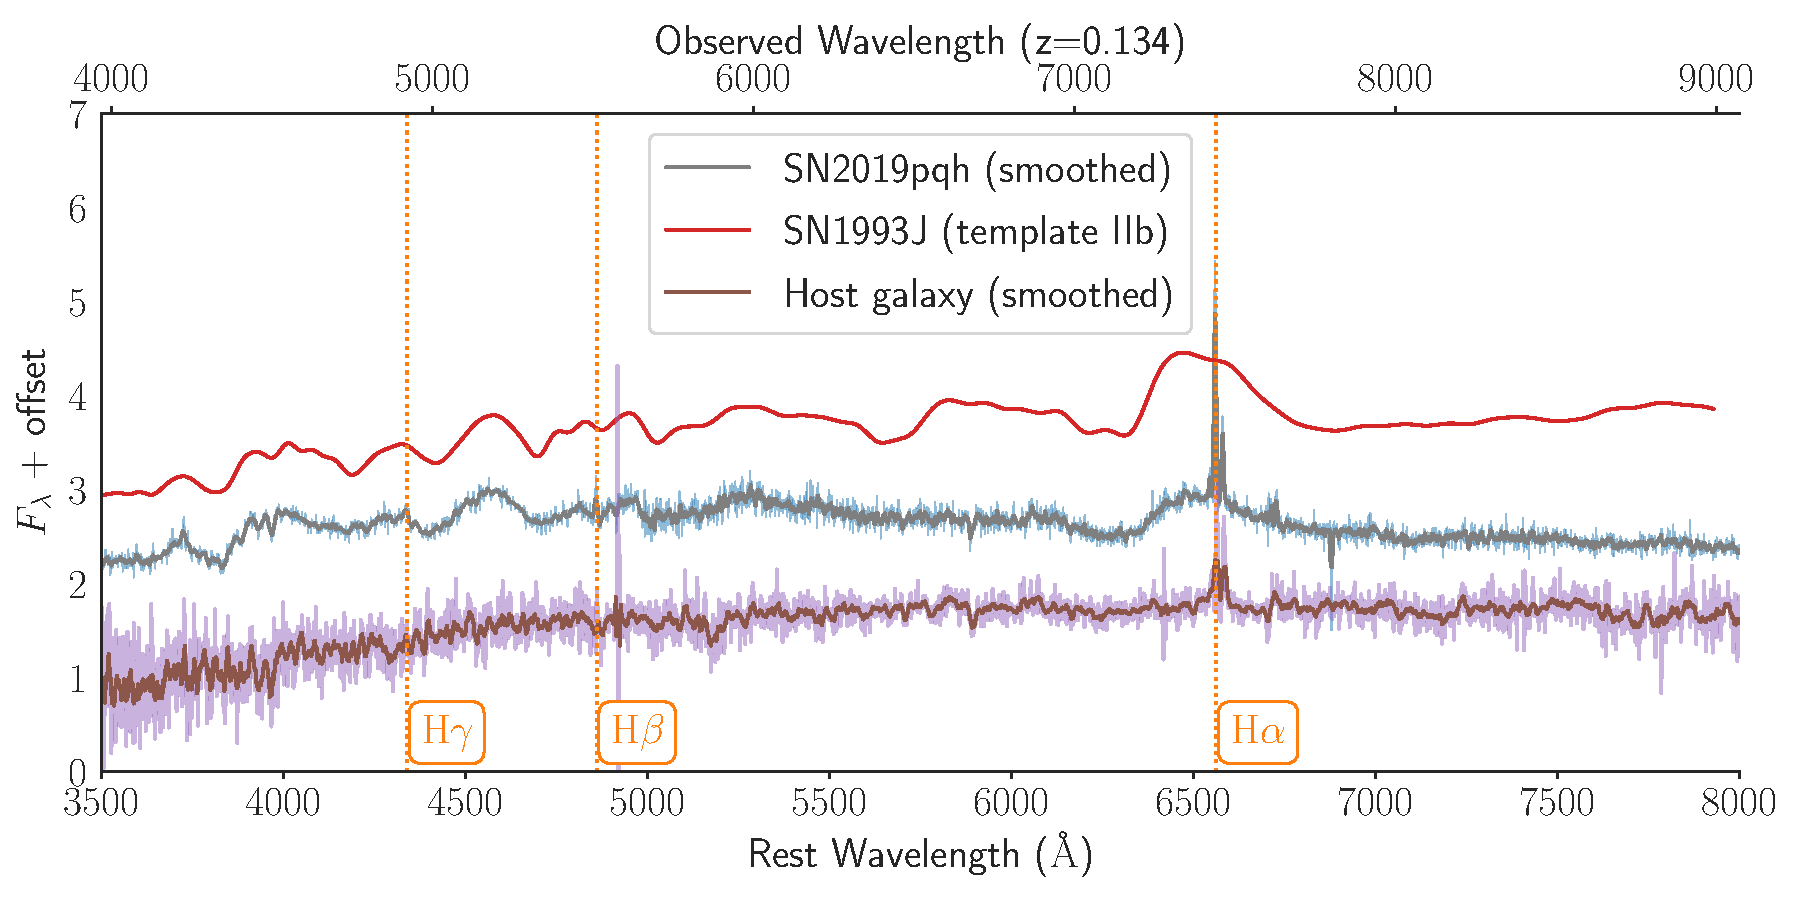
\includegraphics{ZTF/sn2019pqh_spectrum}
	\caption{Spectrum of SN2019pqh, taken on x. The prominent Balmer lines are highlighted in orange, from which a redshift of 0.134 is derived. A template-matching classification using SNID yields a match to a Type IIb supernova (SN1993J) 2 days before peak cite. }
	\label{fig:sn2019pqh_spectrum}
\end{figure}

\subsection{AT2019fdr}

ZTF serendipitously observed the localisation of neutrino IC200530A just 10 minutes after detection, as part of routine survey operations\cite{IC200530A}. Additional ToO observations were then conducted on 2020 May 31 in g- and r-band, and again on 2020 June 1. At this point AT2019fdr was identified by the pipeline as a candidate neutrino source  \sidecite{ztf_IC200530A}. The transient AT2019fdr had originally been discovered by ZTF on 2019 May 03 \cite{at2019fdr_ampel_disc}, but remained in a significantly-elevated flux state at the time of neutrino detection (see Figure \ref{fig:AT2019fdr_lightcurve}). 

\begin{figure}[!ht]
	\centering 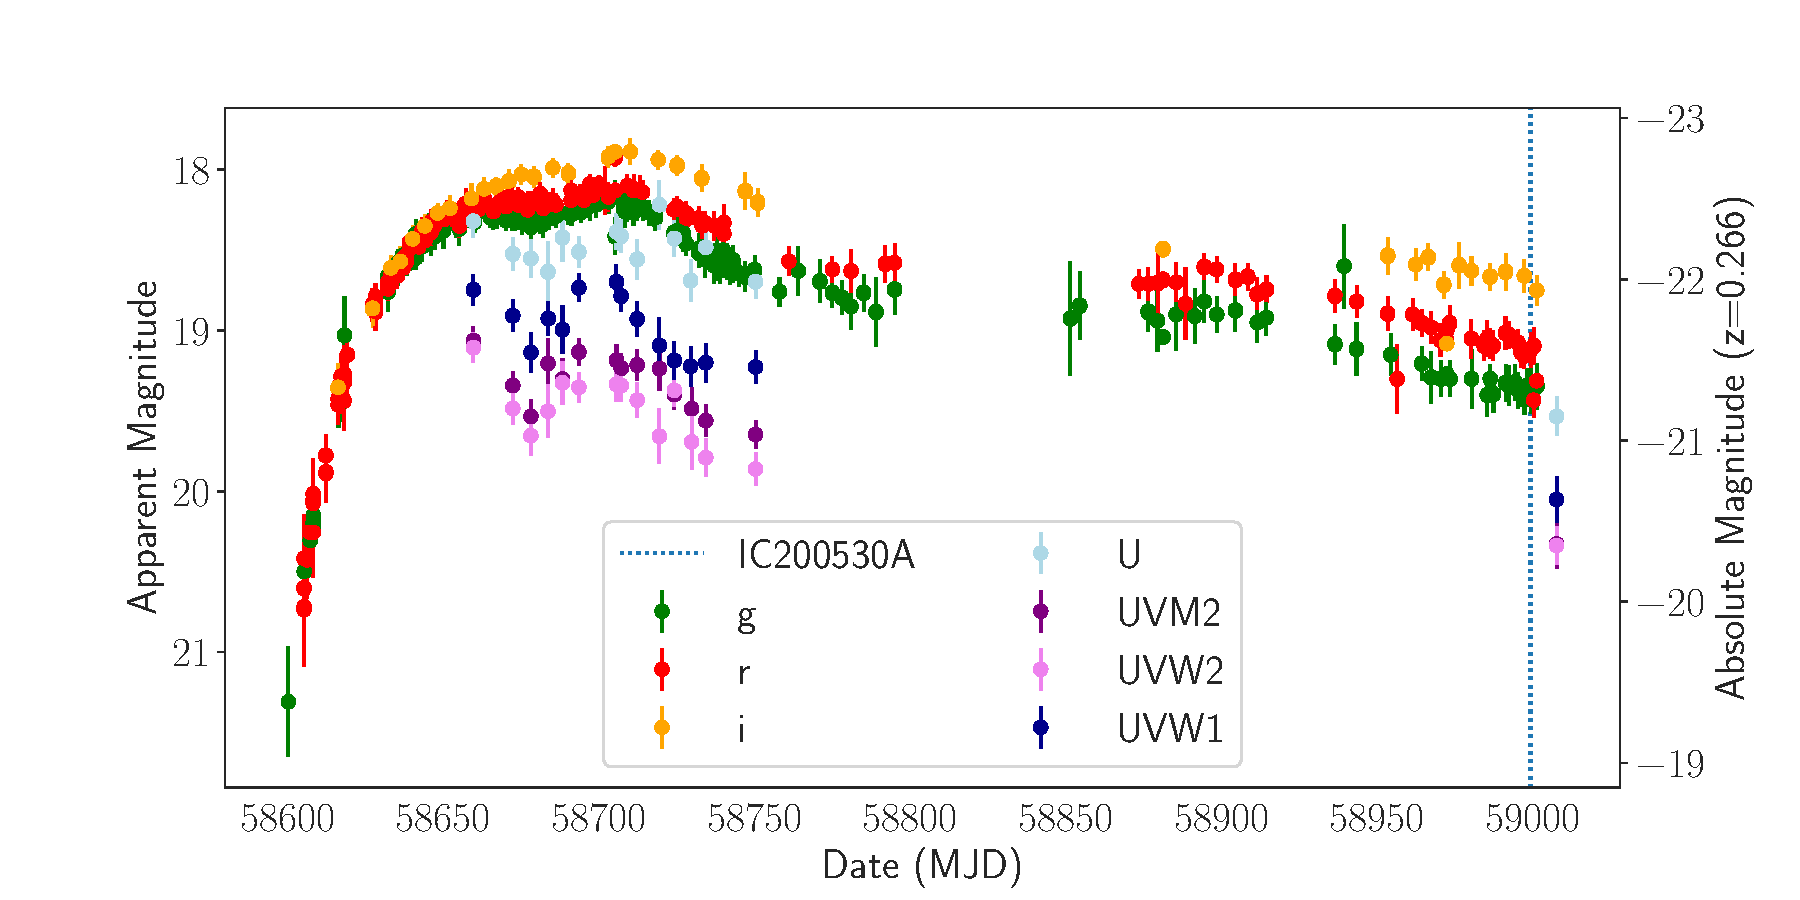
\includegraphics{ZTF/AT2019fdr_lightcurve}
	\caption{ZTF lightcurve of AT2019fdr, with observations in g, r and i band. Photometry from Swift-UVOT is also shown. The arrival time of the neutrino on 2020 May 30 is marked with a dotted line, and the supernova is detected in the subsequent ToO obsersations, for both ZTF and Swift.}
	\label{fig:AT2019fdr_lightcurve}
\end{figure}

A spectrum of the object was taken on 2019 June 8, which gave an ambiguous classification but found a redshift of 0.267 on the basis of nebular emission lines (see Figure \ref{fig:spectra}). Given the consistency of the transient position with the host nucleus, and the bright nature of transient, there was initially considerable interest in this object as a possible TDE or superluminous supernova (SLSN). As can be seen in Figure \ref{fig:AT2019fdr_lightcurve}, the transient peaked at an absolute magnitude of -22.8 in i-band, with little apparent fading through to the detection of the neutrino 10 months later. 

The object was tentatively classified as a luminous Type IIn supernova, though the possibility of an AGN classification was also mentioned \cite{at2019fdr_tns_class}.
Given the lack of temperature evolution over the subsequent 10 months of observation, a supernova classification seems unlikely. Instead, AT2019fdr more likely belongs to a recently-identified class of flares in Narrow-line Seyfert galaxies \sidecite{trakhtenbrot19}. Indeed, our late-time spectroscopy (Figure \ref{fig:spectra}) reveals iron emission lines  characteristic of these flares.

Flares that fall into the spectroscopic class defined by \cite{trakhtenbrot19} all occurred in Narrow-Line Seyfert\,1 (NLS1) galaxies. They show a large long-duration flare which leads to a sustained flux increase on timescales of many months, with little apparent temperature or color evolution. Such flares also have characteristic spectroscopic features, namely emission lines at $\lambda4640$ and $\lambda4686$ as well as an OIII-complex, which distinguish them from other objects. These signatures are also present for AT2019fdr (red and blue lines in Figure \ref{fig:at2019fdr_spectra}).

To date, ZTF has identified 5 large outburst from NLS1's. Accounting for all neutrinos followed-up by ZTF, \textbf{the probability that such a flare should be found by chance is just 0.9\%}. It is thus likely that AT2019fdr is indeed the source of IC200530A. AT2019fdr is the first NLS1 flare reported in spatial and temporal coincidence with a high-energy neutrino. However, neutrino emission has been predicted theoretically from Seyfert galaxies \cite[see e.g][]{murase_agn}. Indeed, in light of AT2019dsg, recent theoretical work has suggested that tidal disruption events may share a common neutrino production mechanism with active galaxy cores \sidecite{murase_bran}. 

Observations of AT2019fdr contemporaneous with the neutrino detection are needed to enable comprehensive modelling of the object, and identify possible mechanisms for neutrino production. Radio observations could again reveal the presence of an outflow, found for AT2019dsg and independently proposed for these flares \cite{trakhtenbrot19}. Such outflows may indeed be the key signature of neutrino production. Conversely, a radio non-detection would strongly disfavour the association of this object with IC200530A.

\subsection{SN2020xxx}

Two likely supernovae were also identified by the pipeline \cite{ztf_IC200530A}, but this is compatible with background expectations, and one has since been firmly excluded as a neutrino counterpart through spectroscopic classification. The other...

\section{Gravitational Waves and Gamma-ray Bursts}
In contrast to neutrinos, follow-up of GW and GRB triggers is more akin to searching for a needle in a haystack. The localisations tend to be much larger than for neutrinos, but with the well-defined aim of finding kilonovae. In this case, we at least know what our needle looks like. GW170817 provided an observational confirmation of theoretical predictions of kilonovae, namely that they are faint, fast-evolving, red transients which are generated following mergers of neutron stars. Though a trigger event may cover several hundred or thousand square degrees, these constraints enable us to efficiently reject the vast majority of candidates. Additional temporal coincidence is ensured by requiring that candidates are not detected prior to merger/burst, and spatial coincidence can be ensured using trigger probability skymaps integrated out to predefined confidence intervals (typically 90\% or 95\%). Unique among triggers, GW events are also typically reported with estimated distance ranges derived from template-matching. For candidates which have a resolved host galaxy, we can determine their distance using spectroscopic surveys such as SDSS, as well as photometric redshift estimates, and veto those candidates lying outside the desired distance range.

The third observing run of the LIGO/VIRGO (O3) extended from X to y, and for this period ZTF has followed-up LVc GW triggers. In this period, there were BNs candidates and Y BBH candidates.

There have been some predictions of EM signatures for BBH events...

\begin{table*}
	\centering
	\begin{tabular}{||c c c c c c c c c c||} 
		\hline
		\textbf{Name} & \textbf{P$_{\textup{t}}$} & \textbf{Area} & \textbf{Distance} & \textbf{Class} & \textbf{P$_{\textup{1}}$} & \textbf{P$_{\textup{2}}$} & \textbf{Time Lag} & \textbf{Depth} & \textbf{E(B$-$V)}\\
		&&(sq. deg.)&(Mpc)&&&&(hr)&&\\
		\hline
		GW190425 &  1\% & 7461  & 156 $\pm$ 41& BNS & 24.13\%  & 23.90\%  & 0.003& 21.5 & 0.03\\
		S190426c & 58\% & 1131  & 377 $\pm$ 100 & NSBH & 52.33\%  & 51.57\% & 13.06& 21.5 & 0.34\\
		S190814bv & 1\% & 23  & 267 $\pm$ 52 & NSBH & 88.57 \%  &  78.37\%  & 0.00 & 21.0 & 0.02\\ % check this
		S190901ap & 14\% & 14753  & 241 $\pm$ 79  & BNS & 56.94\% & 49.39\%  & 3.61& 21.0 & 0.03\\
		S190910d & 2\% & 2482 & 632 $\pm$ 186  & NSBH & 32.99\% & 31.17\%& 1.51& 20.3 & 0.04\\
		S190910h & 39\% & 24264 & 230 $\pm$ 88 & BNS & 33.26\%  & 28.92\% & 0.015& 20.4 & 0.08\\
		S190923y & 32\% & 2107  & 438 $\pm$ 133& NSBH & 38.99\%  & 19.22\% & 13.73& 20.1 & 0.09\\
		S190930t & 26\% & 24220  & 108 $\pm$ 38 & NSBH & 50.63\% & 43.42\% & 11.91& 21.1 & 0.05\\
		S191205ah & 7\% & 6378  & 385 $\pm$ 164  & NSBH & 5.68\% & 4.85\% & 10.66& 17.9 & 0.04\\
		S191213g & 23\% & 4480 & 201 $\pm$ 81  & BNS & 27.50\%  & 25.10\% & 0.013& 20.4 & 0.30\\
		S200105ae & 97\%& 7373  & 283 $\pm$ 74  & NSBH & 52.39\% & 43.99\%  & 9.96 & 20.2 & 0.05\\
		S200115j & 1\% & 765 & 340 $\pm$ 79 & NSBH & 22.21\% & 15.76\%  & 0.24 & 20.8 & 0.13\\
		S200213t & 37\% & 2326  & 201 $\pm$ 80& BNS & 72.17\% & 70.48\%  & 0.40 & 21.2 & 0.19\\
		\hline
	\end{tabular}
	\caption{Summary of ZTF follow-up of 13 gravitational wave events in O3. We list the GW False Alarm Rate (FAR) and in parantheses, the probability that the event is terrestrial (P$_{\textup{t}}$). We list the total size of the GW localization region, the GW median distance and the most probable GW classification. We report the integrated probability within the 90\% contour of the LALinference skymap, covered by triggered and serendipitous ZTF searches during the first three days after merger observed at least once (P$_{\textup{1}}$), and probability observed at least twice (P$_{\textup{2}}$). In parentheses, we include the coverage based on the BAYESTAR skymap. For some events, only BAYESTAR skymaps were made available. All estimates correct for chip gaps and processing failures. We also report the time lag between merger time and start of ZTF observations (hours), the median depth (AB mag), and the median line-of-sight extinction.}
	\label{tab:gw_alerts}
\end{table*}

\setchapterpreamble[u]{\margintoc}
\chapter{AT2019dsg and IC191001A}
\labch{bran}

On 2019 October 1, the IceCube Neutrino Observatory reported the detection of a $\sim$0.2 PeV neutrino, IC191001A, with a 59\% probability of being of astrophysical origin \cite{stein:gcn25913} (see Chapter \ref{ch:realtime}). Seven hours later, the direction of the incoming neutrino was observed by ZTF as part of our neutrino follow-up program. The data was processed by our multi-messenger pipeline (see Chapter \ref{ch:ztf_too}) and the radio-emitting tidal disruption event AT2019dsg was identified as a candidate neutrino source \cite{2019ATel13160....1S}.

\section{Discovery of AT2019dsg}

AT2019dsg was discovered by ZTF on 2019 April 9 under the name \emph{ZTF19aapreis}, and reported on 2019 April 22 as a likely extragalactic transient by AMPEL \sidecite{2019TNSTR.615....1N}. AT2019dsg was publically classified as a TDE on 2019 May 13 by ePESSTO+ on the basis of its optical spectrum\sidecite{2019ATel12752....1N}.  All candidate TDEs identified by ZTF are named after characters from HBO series \emph{Game of Thrones}. As the nth candidate TDE, AT2019dsg was given the official nickname of \emph{ZTF-BranStark} \sidecite{2020arXiv200101409V}. 

Radio emission was tentatively reported on 2019 May 23 by AMI-LA \cite{2019ATel12798....1S}, and confirmed on 2019 July 26 by e-MERLIN \cite{2019ATel12960....1P}. The potential neutrino association was reported on 2019 October 2 \sidecite{2019ATel13160....1S}. In addition to observations as part of a systematic ZTF search for TDEs \cite{2020arXiv200101409V}, the association with IC191001A prompted additional follow-up. 

\section{Observation of AT2019dsg}

\begin{figure}[!ht]
	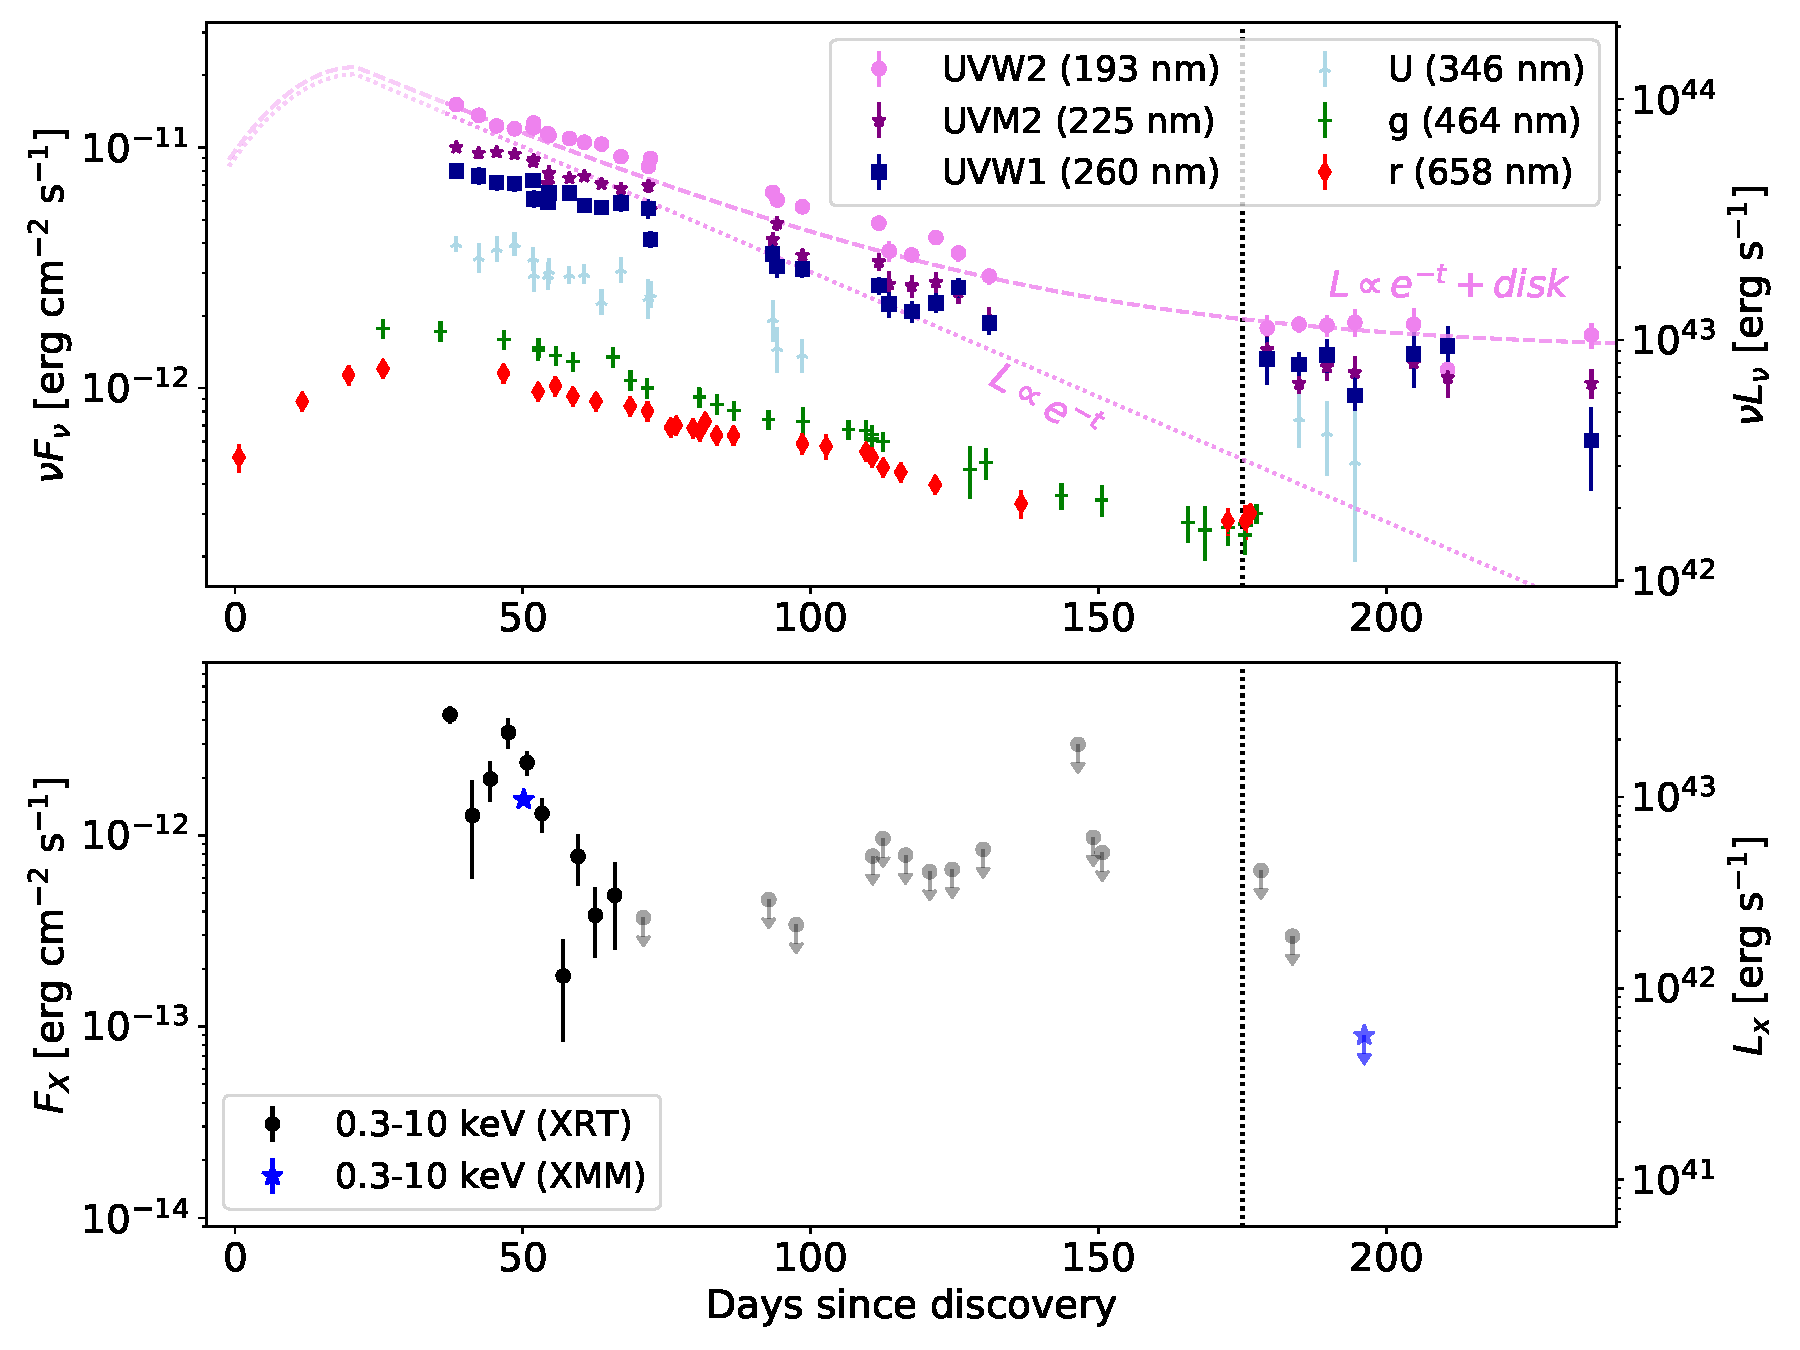
\includegraphics{Bran/lightcurve_wfit.pdf}
	\caption{Multi-wavelength lightcurve of AT2019dsg. Error bars represent 1$\sigma$ intervals. The upper panel shows the optical photometry from ZTF, alongside UV observations from \textit{Swift}-UVOT. The plateau luminosity is a factor of 10 brighter in UVW2 than the pre-disruption baseline of the host galaxy. The lower panel shows the integrated X-ray energy flux, from observations with \textit{Swift}-XRT and \textit{XMM-Newton}, in the energy range 0.3-10 keV. Arrows indicated 3$\sigma$ upper limits.  The vertical dotted line illustrates the arrival of IC191001A.}
	\label{fig:bran_lightcurve}
\end{figure}

\subsection{Optical/UV}

 The optical/UV continuum of AT2019dsg is well described by a single blackbody photosphere with a near-constant temperature \cite{2020arXiv200101409V} of $10^{4.59 \pm 0.02}$~K and radius of $10^{14.59 \pm 0.03}$~cm. The peak luminosity of $10^{44.54 \pm 0.08}$ erg\,s$^{-1}$ is in the top 10\% of the 40 known optical TDEs to date \cite{2020arXiv200101409V}, and the temperature is in the top 5\%. By the time of the neutrino detection, the optical/UV luminosity appeared to have reached a plateau (see Figure \ref{fig:bran_lightcurve}). Such plateaus are common in TDEs and interpreted as emission from the outer part of an accretion disk \cite{2019ApJ...878...82V,2020MNRAS.492.5655M}, but typically occur a few years after peak. The rapid appearance of an accretion-disk plateau would be expected for disruptions around higher-mass SMBHs. Indeed the total mass of the host galaxy of AT2019dsg is in the top 10$\%$ of all optical TDE hosts. Assuming 50$\%$ of the host mass is in the bulge, we estimate \cite{2013ApJ...764..184M} a black
hole mass of $\sim 3 \times 10^{7} \Msol$.

Prior to the detection of IC191001A, AT2019dsg had already been repeatedly detected by ZTF P48 telescope as part of the public MSIP survey, most recently on 2019 September 28. These data were supplemented by photometric observations from the 2m Liverpool Telescope\cite{2004SPIE.5489..679S} and SEDM\cite{Blagorodnova18,Rigault19} photometry\cite{fst+2016} obtained using the P60 telescope on Mt Palomar. ToO observations of the neutrino localisation field began on 2019 October 1, 7.4 hours after the neutrino detection. A second set of observations were performed the following night. In all of these images AT2019dsg was clearly visible. 

UV observations of AT2019dsg were conducted as part of a systematic survey of UV properties of all ZTF-identified TDEs\cite{2018ApJ...852...72V}, using the UltraViolet/Optical Telescope\cite{2005SSRv..120...95R} (UVOT) on board the \textit{Neil Gehrels Swift Observatory} (\textit{Swift})\cite{2004ApJ...611.1005G}. Data were reduced with \texttt{uvotsource} using an aperture of 7" to capture the entire galaxy (the host flux density was subtracted based on the best-fit galaxy model\cite{2018ApJ...852...72V} and uncertainties on this baseline are propagated into the reported UVOT difference photometry). The first UV observation was performed 15 days after the optical peak on 2019 May 17, and a bright source spatially coincident with the TDE was detected. Subsequent observations continued at a cadence of 2--3 days, up to 2019 September 7. In this period, AT2019dsg continued to steadily dim. An additional observation occurred shortly before the neutrino detection on 2019 September 27. Follow-up observations were then triggered by the identification of a possible association with IC191001A\cite{2019ATel13160....1S}, beginning on 2019 October 5. 

The optical/UV data are summarised in Table \ref{tab:photometry}. We note that in the final ZTF observations, the source appears to redden in the optical bands. This could be a signature of reverberation due emission from dust heated by the TDE\cite{2016ApJ...829...19V,2016MNRAS.458..575L}; this dust can reach a temperature of $\sim 2000$ K. An important caveat is that the contrast between the transient emission and the host is very small for these late-time optical detections, so the residuals in the difference image may need to be corrected to account for small systematic offsets. That can only be investigated when the images for this portion of the public survey are published as part of the next ZTF data release. We note that the UV observations are not subject to the same uncertainty because even at late times the transient UV flux is about an order of magnitude brighter than the host baseline.

\subsection{X-ray}

AT2019dsg was also detected in X-rays, beginning 37 days after discovery. Though the first X-ray observation indicated a bright source, with a high X-ray to optical ratio of $L_{\textup{X}}/L_{\textup{opt}} \sim $0.1, this X-ray flux faded extremely rapidly, as shown in Figure \ref{fig:bran_lightcurve}. This rate of decline is unprecedented, with at least a factor of 50 decrease in X-ray flux over a period of 159 days. Similar to the optical/UV emission, the observed X-ray spectrum is consistent with thermal emission, but from a blackbody of temperature $10^{5.9}$ K ($0.072 \pm 0.005$ keV) and, assuming emission from a circular disk, a radius $\sim 2 \times 10^{11}$ cm. As for most X-ray-detected TDEs\cite{2017ApJ...838..149A, 2019MNRAS.487.4136W,2019ApJ...872..198V}, the blackbody radius appears much smaller than the Schwarzschild radius ($R_{\textup{S}} \sim 10^{13}$~cm) inferred from the galaxy scaling relation\cite{2013ApJ...764..184M}. Small emitting areas can arise from an edge-on orientation, because the relativistic velocities at the inner disk can Doppler boost a large area of the disk out of the X-ray band.  Since our observations probe close to the Wien tail of the spectrum, a small temperature decrease due to absorption would also yield a significantly underestimated blackbody radius and luminosity\cite{2019ApJ...872..198V}. The exponential decrease of the flux could be caused by cooling of the newly-formed TDE accretion disk\cite{2020MNRAS.492.5655M} or increasing X-ray obscuration.

AT2019dsg was first observed in X-rays on 2019 May 17 by the X-Ray Telescope (XRT)\cite{2005SSRv..120..165B}, also on board \textit{Swift}\cite{2004ApJ...611.1005G}, as part of a program to categorise the X-ray properties of TDEs. AT2019dsg was detected at high significance at this epoch, with a measured energy flux of $F_{X}\sim 4 \times 10^{-12}$ erg cm$^{-2}$ (0.3--10 keV). Observations continued with a cadence of 2--3 days, and indicated a sharply-declining X-ray flux. The source was last detected on 2019 June 14, and not detected again in any of the following observations continuing until 2019 September 7. An additional observation was performed with the \textit{X-ray Multi-Mirror Mission} (\textit{XMM-Newton}) telescope on 2019 May 30, in the range 0.3-10 keV. The \textit{XMM-Newton} EPIC-pn observations (programs 082204 and 08425; P.I. Gezari) were taken in Wide window Thin1 filter mode and reduced using standard techniques with the \textit{XMM-Newton}\cite{2001A&A...365L...1J} Science Analysis System (SAS). The source extraction region was a circle of radius 35 arcsec at the location of the optical transient in the X-ray image, and the background was measured using a 108-arcsec circular region (shown in Figure \ref{fig:xraymap}). The \textit{XMM} spectrum was binned using the \texttt{GRPPHA} command, such that there were at least 20 counts contained in each bin. It was then fit ($\chi^2/\textup{dof}=59.26/65$) with the  disk blackbody (\texttt{diskbb}) model with Galactic\cite{HI4PI2016} and intrinsic ($N_{\textup{H}} \sim 4 \times 10^{20}$ cm$^{-2}$) absorption described using the \texttt{phabs} model in \texttt{XSPEC} v12.9.1\cite{1996ASPC..101...17A}. The flux was consistent with those of \textit{Swift}-XRT, and provided a high signal-to-noise X-ray spectrum well-fitted with a single disk temperature of $T_{\textup{disk}} = 10^{5.9}$ K (0.072 $\pm 0.005$ keV), shown in Figure \ref{fig:xrayspec}. Following the identification of AT2019dsg as a candidate counterpart to IC191001A\cite{2019ATel13160....1S}, additional X-ray observations were triggered. AT2019dsg was again not detected, with the first \textit{Swift}-XRT observation occurring on 2019 October 5. An additional \textit{XMM} observation on 2019 October 23 yielded a deep upper limit of $9 \times 10^{-14}$ erg cm$^{-2}$ s$^{-1}$ (0.3--10 keV) using the same thermal model, computed at the 3$\sigma$ confidence level using the \textit{XMM} SAS/HEASARC command \texttt{eregionanalyse}. 

\begin{marginfigure}
	\centering
	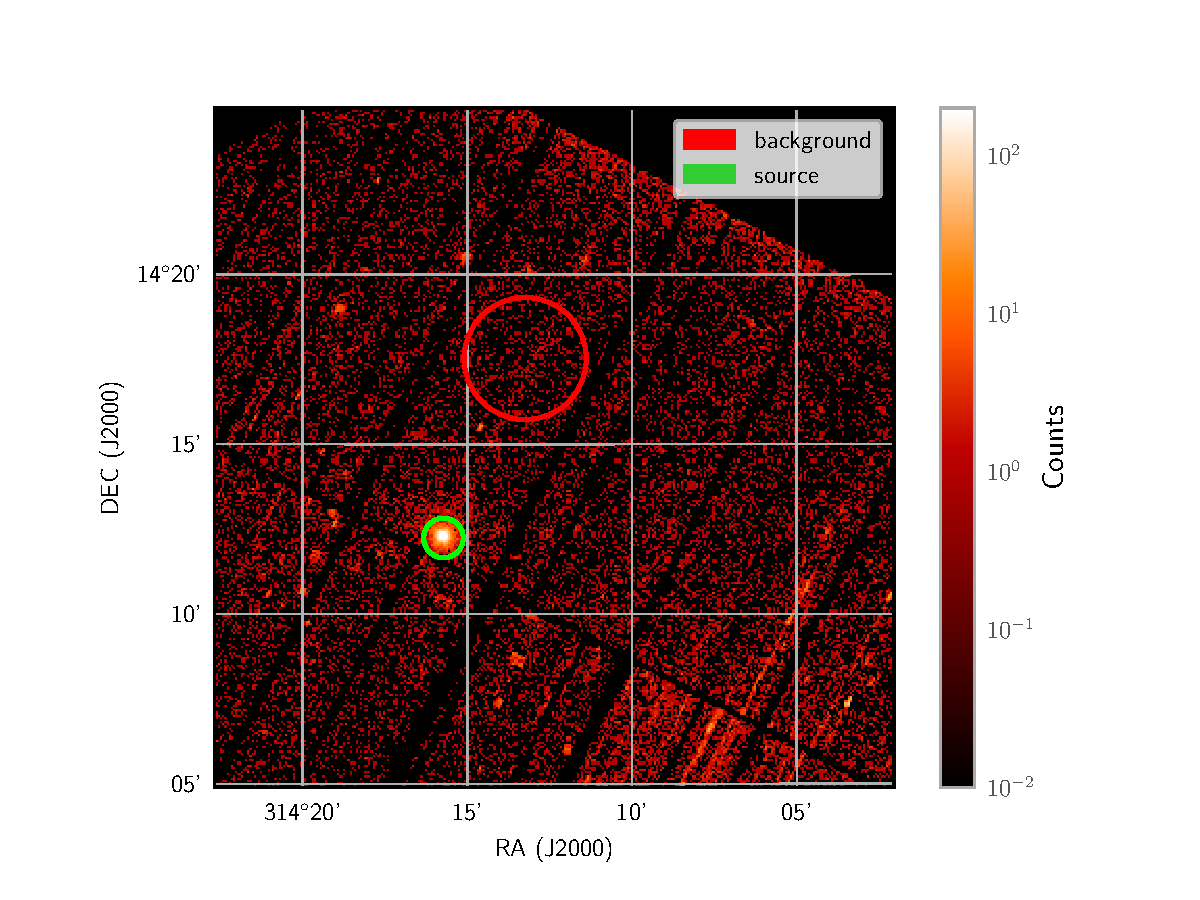
\includegraphics{Bran/Bran_XMM_epoch1_region.pdf}
	\caption{X-ray count map from \textit{XMM-Newton} (50 days after discovery). The green circle indicates the source region, while the red circular region was used to measure the background. The best-fit position derived from optical observations is spatially-coincident with the center of the X-ray source region.}
	\label{fig:xraymap}
\end{marginfigure}

\begin{figure*}
	\centering
	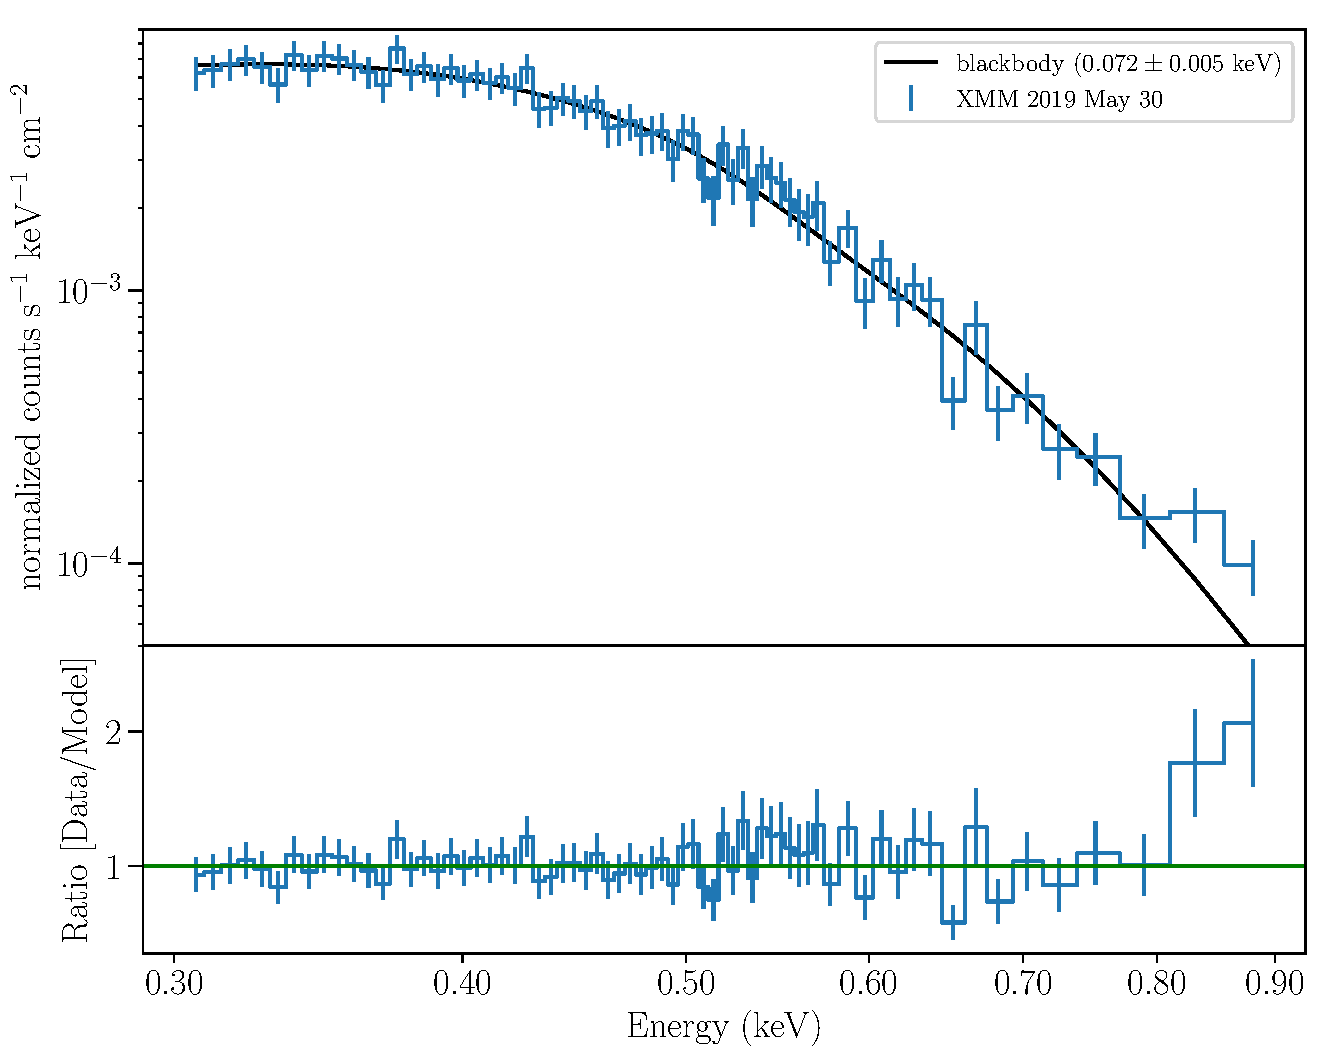
\includegraphics[width=0.95\textwidth]{Bran/3eyedraven_xmm_spc_0842590901_abs.pdf}
	\caption{Soft X-ray spectrum of AT2019dsg measured by \textit{XMM-Newton}, fitted with an absorbed disk blackbody model. Error bars represent 1$\sigma$ intervals.}
	\label{fig:xrayspec}
\end{figure*}

\subsection{Radio}

Radio observations shown in Figure \ref{fig:radio_spectrum} reveal a third distinct spectral component, namely synchrotron emission from non-thermal electrons. We model this emission with a  conical geometry as expected for outflows (e.g., jets or winds) that are launched from---and collimated by---the inner parts of flared accretion disks that emit close to the Eddington limit.
Given that electrons are typically accelerated with much lower efficiency than protons in astrophysical accelerators\cite{2012A&A...538A..81M}, we assume that they carry 10\% of the energy carried by relativistic protons ($\epsilon_{e} = 0.1$). We further assume that the magnetic fields carry 0.1\% of the total energy ($\epsilon_{B} = 10^{-3}$), as indicated by radio observations of other TDEs\cite{2018ApJ...854...86E} and supernovae\cite{2013MNRAS.436.1258H}. For a half-opening angle, $\phi$, of 30\arcdeg\ we find $R = 1.5 \times 10^{16}$ cm in our first epoch (41 days after discovery), increasing to $R = 7 \times 10^{16}$~cm shortly after the neutrino detection (177 days after discovery).  These radii scale\cite{2013ApJ...772...78B} as $R \propto [1-\cos(\phi$)]$^{-8/19}$. The implied expansion velocity is roughly constant at $v/c = \dot{R}/c = 0.12 \pm 0.01 $ during the first three epochs, with an acceleration to $v/c = 0.21 \pm0.02$ for the last epoch.  These are the velocities of the synchrotron-emitting region, and thus provide a lower limit to the velocity at the base of the outflow.  Indeed even the hotspots of relativistic jets from active galaxies that are frustrated by gas in their host galaxy are typical observed\cite{2003PASA...20...69P} to have subrelativistic expansion velocities of $\sim0.1c$. 

The inferred outflow energy, $E$, shows a linear increase from $2.5 \times 10^{49}$~erg to $2 \times 10^{50}$~erg (Figure \ref{fig:radio_spectrum}), which is not expected in models\cite{2016ApJ...819L..25A,2016ApJ...827..127K} of TDE radio emission that involve a single injection of energy. While some scenarios can yield an increase in inferred energy from a single energy injection, none of these are consistent with the full set of observed properties. First, a single ejection with a range of velocities could explain the observed linear increase of energy with time (the slower ejecta arrive later), but is incompatible with the increasing velocity. Second, an increase of the efficiency for conversion of Poynting luminosity to relativistic particles is unlikely because the target density that is available to establish this conversion is decreasing.  And finally, an increase of solid angle that emits to our line of sight is only expected for relativistic outflows that decelerate. Instead, for AT2019dsg, the observations suggest the presence of a central engine that yields continuous energy injection through a coupling of accretion power to the radio emission\cite{2018ApJ...856....1P}, with acceleration in the final radio epoch due to a decrease in the slope of the ambient matter density profile. 

Four observations of AT2019dsg were performed with the Karl G.\ Jansky Very Large Array (VLA) under project code 19A-395 (PI: van~Velzen), on 2019 May 22, June 19, August 8 and October 5.  The array was in its moderately-extended B configuration (maximum baseline 11\,km) for the first two epochs, and in its most extended A-configuration (maximum baseline 36\,km) for the final two epochs.  Our first epoch, on May 22, was a detection experiment, and we observed only in the 8--12\,GHz band.  Having established the presence of radio emission, we observed over a broader range of frequencies in the subsequent three epochs, using the 2--4\,GHz, 4--8\,GHz, and 8--12\,GHz bands.  We used 3C\,48 as a bandpass and flux density calibrator on May 22, and 3C\,286 for the other three epochs.  We used the nearby extragalactic sources ICRF J204945.8+100314 
% MFB: we should give source names that resolve on e.g. Simbad, and good to mention its an ICRF source - our posn accuracy should be good.
(at 4--8 and 8--12\,GHz) and ICRF J203533.9+185705 (at 2--4\,GHz) to determine the complex gain solutions, which were interpolated to AT2019dsg. We used the Common Astronomy Software Application (CASA)\cite{McMullin2007} Calibration pipeline (v5.4.1) to perform external gain calibration, and after removing residual radio frequency interference, we imaged the data within CASA, using Briggs weighting with a robust parameter of 1.  We split each baseband into multiple frequency bins for imaging (1\,GHz bins above 4\,GHz, and 0.5\,GHz bins below that) to provide better sampling of the broadband spectrum, allowing more precise constraints on the turnover frequency, and better spectral modelling.

% two paragraphs from AMI 
Radio observations of the field of AT2019dsg were also conducted using the AMI Large Array (AMI-LA)\cite{2008MNRAS.391.1545Z,2018MNRAS.475.5677H}. AMI-LA is a radio interferometer comprised of eight 12.8m-diameter antennas producing 28 baselines that range from 18m up to 110m, which operates with a 5 GHz bandwidth around a central frequency of 15.5 GHz. We observed AT2019dsg on several epochs (see Table \ref{tab:radio_data}) for four hours each. Initial data reduction, editing, and calibration of the phase, and flux density, was carried out using \verb reduce_dc , a customized AMI data reduction software package\cite{2015MNRAS.453.1396P}. Phase calibration was conducted using short interleaved observations of ICRF J205135.5+174336,
%MFB was: J2051+1743, 
while for absolute flux density calibration we used 3C\,286. Additional flagging and imaging were performed using CASA. All of our observations showed a source consistent with the location of AT2019dsg. We used the CASA task IMFIT to find the source flux and position. 

Further observations of AT2019dsg were conducted with the South African MeerKAT telescope, on 2019 June 19, July 29, October  5, and November 30, with each session being $\sim$2~h long.  We used ICRF J193925.0-634245 as a flux-density calibrator, and ICRF J213032.8+050217 as a phase and amplitude calibrator.  The initial calibration was done using the IDIA MeerKAT pipeline\footnote{\url{https://idia-pipelines.github.io/docs/processMeerKAT}}, which is implemented in CASA\@.  The observed band was 860 MHz wide and centred on 1280 MHz. We imaged the whole primary beam ($\sim 1$\arcdeg) using the CLEAN algorithm (CASA: tclean) in order to remove sidelobes from the many (unrelated) sources within the primary beam.  The total CLEAN flux density in the field was $\sim$1~Jy, and the peak brightness in the images was about 48 mJy~beam$^{-1}$ (not related to AT2019dsg). Since residual small calibration errors dominated the image rms background in the initial images, we self-calibrated the data in both phase and amplitude, with the mean amplitude gain being fixed at unity to minimise any drifting of the flux-density scale. The resolution is slightly different in each epoch, but was $\sim$11\arcsec\ north-south, and $\sim$6\arcsec\ east-west.  Image rms background levels also varied, ranging between 25 and 32 $\mu$Jy~beam$^{-1}$.  There was no sign of extended emission or confusing sources near AT2019dsg. The flux density was determined by fitting an elliptical Gaussian with the same geometry as the restoring beam to the images.  

The measured flux densities from our radio observations are reported in Table \ref{tab:radio_data}. For all radio observations, the reported uncertainties include both the image background rms and a 5\% fractional calibration uncertainty, added in quadrature.

\subsection{Gamma-ray}

We analysed data from the %pair-conversion telescope 
\textit{Fermi} Large Area Telescope (\textit{Fermi}-LAT)\cite{2009ApJ...697.1071A}, sensitive to gamma rays with energies from 20 MeV to greater than 300 GeV. During its sky-survey operations, the pair-conversion telescope \textit{Fermi}-LAT scans the entire sky about every three hours, and can monitor the variable gamma-ray sky over short and long timescales. We studied the region of AT2019dsg in three different time intervals, motivated by the multi-wavelength behavior of the source. The first interval (G1) includes 130 days of observations that include the peak of the optical emission from 2019 April 4 to 2019 August 12. The second one (G2) spans 2019 August 12 to 2019 November 20 and covers the UV plateau and the peak of the radio emission. The third period (G3) integrates the whole period between the start of G1 up to 2020 January 31. We use the photon event class from Pass 8 \textit{Fermi}-LAT data (P8R3\_SOURCE), and select a $15\arcdeg \times 15\arcdeg$ Region of Interest (RoI) centered on the AT2019dsg position derived from optical observations, with photon energies from 100 MeV to 800 GeV. We use the corresponding LAT instrument response functions P8R3\_SOURCE\_V2 with the recommended spectral models \textit{gll\_iem\_v07.fits} and \textit{iso\_P8R3\_SOURCE\_V2\_v1.txt} for the Galactic diffuse and isotropic component respectively. To minimise contamination from gamma rays produced in the Earth's upper atmosphere, we require an instrumental zenith angle $\theta<90\arcdeg$ for all events, in addition to the standard data quality cuts suggested by the \textit{Fermi} Science Support Center\footnote{\url{https://fermi.gsfc.nasa.gov/ssc/data/analysis/scitools/data_preparation.html}}. We perform a likelihood analysis, binned spatially with $0.1 \arcdeg$ resolution and 10 logarithmically-spaced bins per energy decade, using the \textit{Fermi}-LAT ScienceTools package (fermitools v1.0.1) along with the \textit{fermipy} package v0.17.4\cite{2017ICRC...35..824W}.

A search was already performed within the 90\%\ error region during both the 1-day and 1-month period prior to the arrival of the high-energy neutrino\cite{garrappa_buson:gcn25932}. No new gamma-ray source was identified, and there was no significant ($\geq 5 \sigma$) detection for any source from the fourth \textit{Fermi}-LAT point source catalog (4FGL\cite{2019arXiv190210045T}). Here, we specifically test a point-source hypothesis at the position of AT2019dsg under the assumption of a power-law spectrum. We find TS\footnote{TS is twice the difference in the maximum $\log \mathcal{L}$ of an ROI model with and without the source, where $\mathcal{L}$ is the likelihood of the data given the model.} = 0 for all intervals. Upper limits for the energy flux (integrated over the whole analysis energy range) have been derived for a power-law spectrum ($dN/dE \propto E^{-\Gamma}$) with photon power-law index $\Gamma$ = 2 and are listed in Table \ref{tab:lat_uls} along with the respective time intervals.

In all three time intervals, we detect a new, non-catalogued gamma-ray emitter in the RoI at a significance $\geq 5 \sigma$. This source lies just outside the IC191001A 90$\%$ error region, as indicated in Figure \ref{fig:fermi}. The source, which we label \textit{Fermi}-J2113.8+1120, is likely the gamma-ray counterpart of the radio-loud object GB6 J2113+1121, classified as a flat-spectrum radio quasar with redshift $z = 1.63$\cite{2013ApJ...767...14P}. The detection of an unrelated gamma-ray blazar within the neutrino uncertainty area is consistent with the background estimation. On average 1.5 4FGL gamma-ray blazars are expected in 20 sq.\,deg. In addition, a lightcurve analysis (Figure \ref{fig:fermi_lc}) reveals that the source is not significantly detected in gamma rays when IC191001A was detected. The lag between the closest significant detection of the source and the neutrino arrival was approximately $\sim$1 month. Such a lag is disfavored by recent studies on the temporal behavior of hadronic processes in blazars\cite{2015ApJ...802..133D,2019NatAs...3...88G}, suggesting that the blazar is unlikely producing the neutrino. %for which a shared origin of GeV photons and high-energy neutrinos from the same processes is disfavoured by recent studies on the temporal behavior of hadronic processes in blazars\cite{2015ApJ...802..133D,2019NatAs...3...88G}. 
Hence, given the lack of any obvious connection between the gamma-ray observations of \textit{Fermi}-J2113.8+1120 and IC191001A, we do not discuss this source any further.

The HAWC observatory also reported a search for transient gamma-ray emission on short timescales in the localisation of IC191001A\cite{ayala:gcn25936}, and set a limit for their most significant position at 95\% confidence of $E^{2} dN/dE = 3.51 \times 10^{-13} (\textup{E}/\textup{TeV})^{-0.3}$ TeV cm$^{-2}$ s$^{-1}$, in the energy range 300 GeV to 100 TeV, for the period from 2019 September 30 05:46:52 UTC to 2019 October 02 06:03:29 UTC. We note that this search covered a relatively large region of the sky, and thus had a large associated trial factor. A dedicated search at the position of AT2019dsg would be more sensitive, especially one that additionally targeted the longer period over which the central engine is active.

\begin{table}
	\centering
	\begin{tabular}{||c c c c||} 
		\hline
		\textbf{Interval} & \textbf{MJD Start} & \textbf{MJD Stop} & \textbf{UL}\\
		& & &  (erg cm$^{-2}$ s$^{-1}$)\\
		\hline
		\textit{G1} & 58577 & 58707 & 2.6 $\times 10^{-12}$\\
		\textit{G2} & 58707 & 58807 & 1.2 $\times 10^{-11}$\\
		\textit{G3} & 58577 & 58879 & 2.0 $\times 10^{-12}$\\
		\hline
	\end{tabular}
	\caption{Gamma-ray energy flux upper-limits for a point-source with power-law index $\Gamma$=2.0 at the position of AT2019dsg integrated over the analysis energy range 0.1-800 GeV.}
	\label{tab:lat_uls}
\end{table}

\begin{figure}
	\centering
	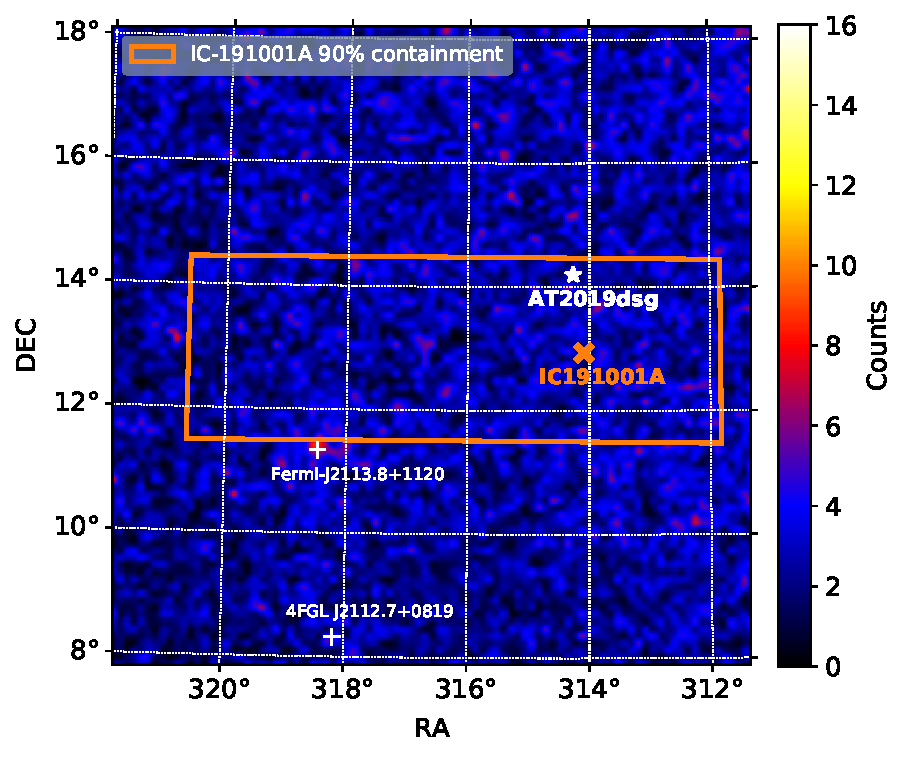
\includegraphics[width=\textwidth]{Bran/LAT_countsmap.pdf}
	\caption{LAT counts map of the Region Of Interest (ROI) in the integrated search period G3, showing the IC191001A 90$\%$ localisation region in green. The neutrino best-fit position is marked with a green `$\times$'. Two gamma-ray sources are significantly detected ($\geq$ 5 $\sigma$) in the ROI but outside the neutrino uncertainty region as marked with white crosses. There is no excess consistent with the position of AT2019dsg. %Gamma-ray sources significantly detected ($\geq$ 5 $\sigma$) are marked with white crosses. 
	}
	\label{fig:fermi}
\end{figure}

\begin{figure}
	\centering
	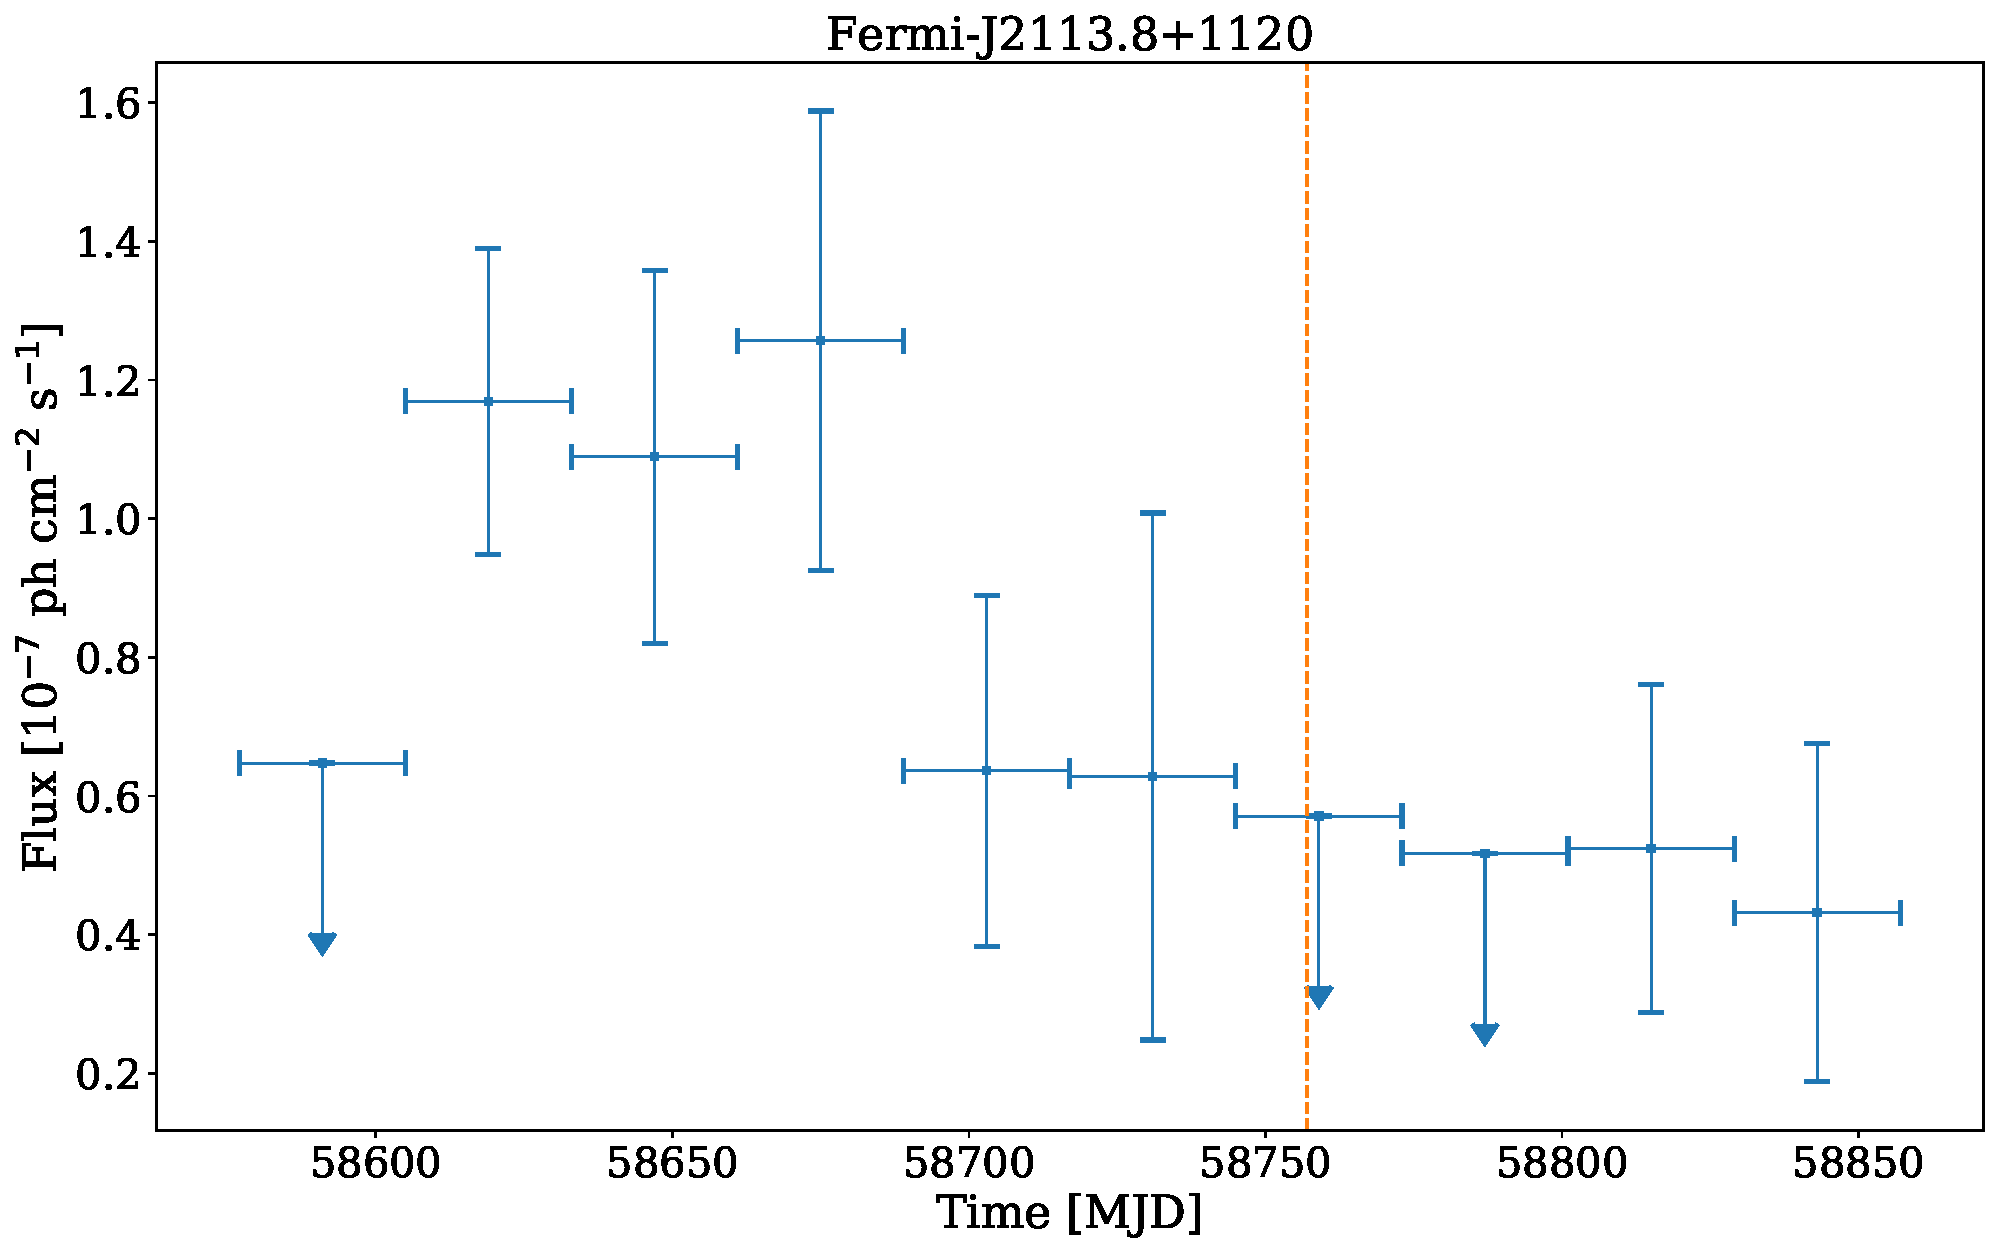
\includegraphics[width=0.8\textwidth]{Bran/fermi_lightcurve}
	\caption{LAT lightcurve in the 0.1-800 GeV energy range for the source \textit{Fermi}-J2113.8+1120 in the time interval G3, with evenly spaced binning of 28 days. Vertical error bars represent 1$\sigma$ intervals, horizontal bars denote bin width. 2$\sigma$ upper limits are shown for bins with TS$\leq$9. The orange dashed vertical line marks the arrival time of IC-191001A. Since this source lies outside the reported 90\% error region (see Figure~\ref{fig:fermi}), and given that the LAT lightcurve shows no obvious correlation with the neutrino arrival time, we conclude that it is unlikely to be associated with the neutrino.}
	\label{fig:fermi_lc}
\end{figure}


\subsection{Spectroscopy}


AT2019dsg was discovered by ZTF on 2019 April 9 under the name ZTF19aapreis, and publically reported as a  \sidecite{2019TNSTR.615....1N}, and was classified as a TDE on the basis of its optical spectrum\cite{2019ATel12752....1N} with a measured redshift of $z=0.051$, implying a luminosity distance $D_{\textup{L}} \approx$ 230 Mpc assuming a flat cosmology with $\Omega_{\Lambda}$ = 0.7 and $H_{0}$ = 70 km s$^{-1}$ Mpc$^{-1}$.

AT2019dsg was first classified as a TDE by ePESSTO+ on on 2019 May 13\cite{2019ATel12752....1N}, and the redshift of AT2019dsg was measured to be $z=0.051$. Further high-resolution spectroscopic observations were conducted using the De Veny Spectrograph on the 4.3m Lowell Discovery Telescope (LDT, PI: Gezari), the Kast Double Spectrograph on the 3m Lick Observatory Shane Telescope (Lick, PI: Foley)\cite{Miller93}, and the Low Resolution Imaging Spectrograph on the 10m Keck Telescope (Keck, PI: Graham)\cite{Oke95}, with the most recent spectrum on 2019 September 25. These spectra confirm that AT2019dsg belongs to the common spectroscopic class of TDEs with Bowen fluorescence emission lines and broad H$\alpha$ emission lines\cite{2020arXiv200101409V}. We note that the Ca triplet is also clearly visible in our late-time spectra (rest-frame 8498 \AA, 8542\AA ~and 8662 \AA), so the SMBH mass could in principle be inferred more precisely using higher-resolution spectroscopy of this feature\cite{2005MNRAS.359..765G}. Following the identification of AT2019dsg as a candidate neutrino source, additional high-resolution spectra of the source were taken with the 200in Hale Telescope Double Spectrograph at Palomar Observatory (P200, PI: Kasliwal \& Kulkarni) on 2019 October 3 and again with  Lick on 2019 October 5 and 2019 October 29 (shown in Figure \ref{fig:bran_spectrum}). There is no evidence of any significant spectral evolution between these spectra and the most recent pre-neutrino spectrum from 2019 September 25, and the spectral evolution of AT2019dsg is consistent with that of other TDEs\cite{2020arXiv200101409V}. 

\begin{figure*}[h!]
	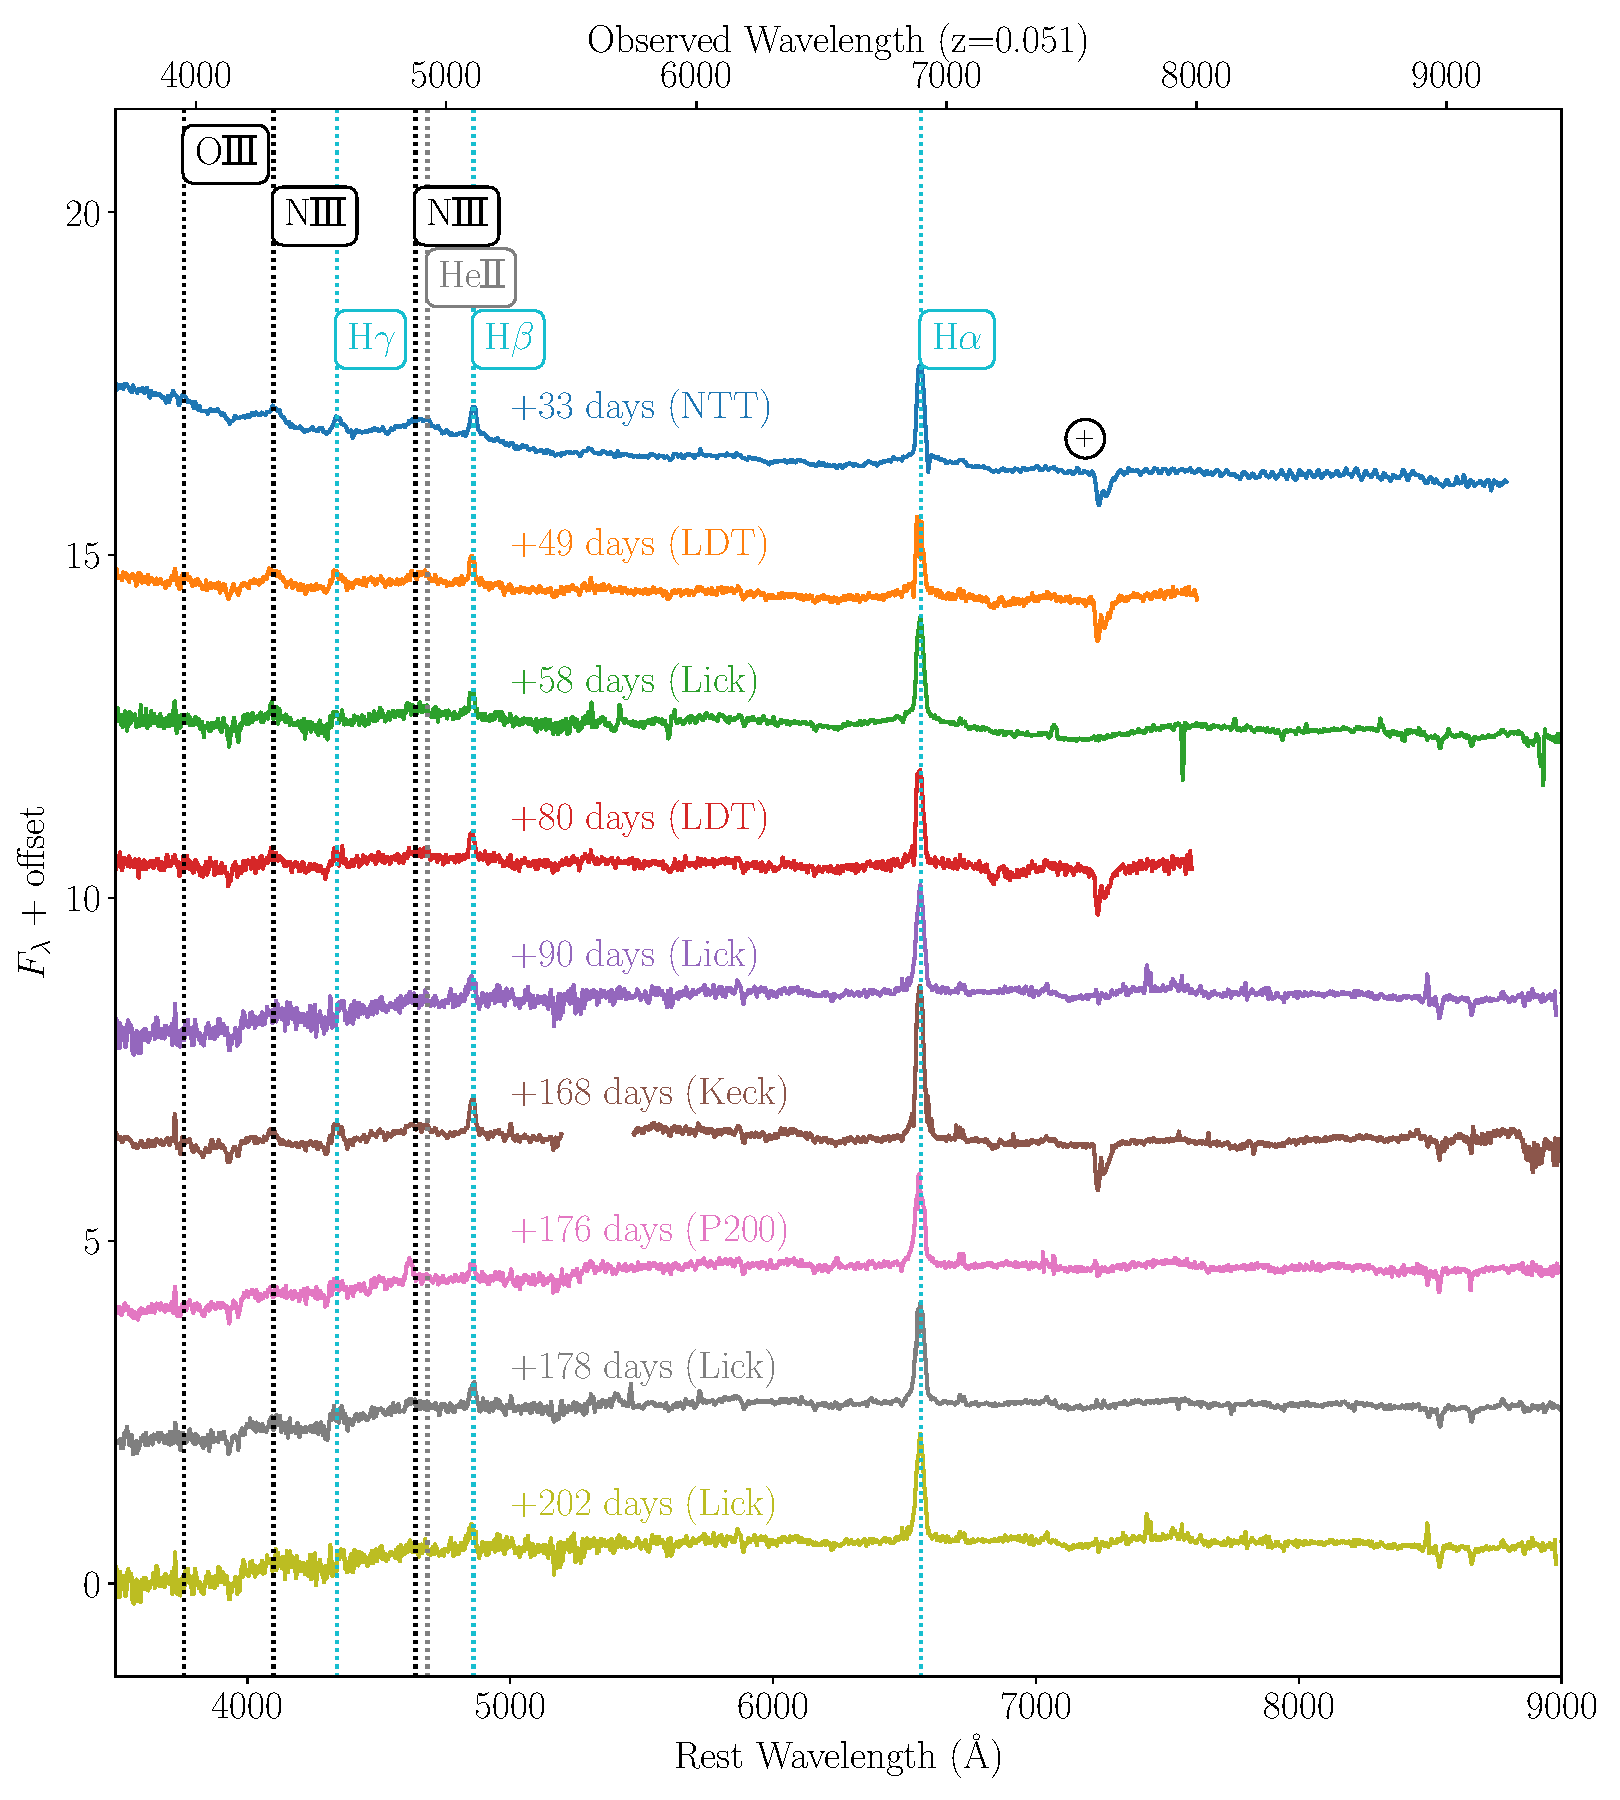
\includegraphics{Bran/spectra.pdf}
	\caption{The spectroscopic evolution of AT2019dsg, beginning with the publicly available classification spectrum taken with the NTT\cite{2019ATel12752....1N}, and further spectra from LDT, Lick, Keck and P200. The Balmer lines are highlighted in cyan, the HeII lines in gray, and the Bowen fluorescence lines (OIII at 3760\AA, NIII at 4100\AA ~and 4640\AA) in black. Telluric lines are marked with +.}
	\label{fig:bran_spectrum}
\end{figure*}

\section{Neutrino emission from AT2019dsg} With this strong evidence for three distinct emission zones derived purely from multi-wavelength observations, we consider whether this picture is consistent with AT2019dsg being the source of the neutrino IC191001A. In particular, neutrino production requires protons to be accelerated to sufficiently high energies, and to collide with a suitably abundant target. The detection of a single high-energy neutrino implies a mean expectation in the range $0.05 < N_{\nu, \textup{tot}} < 4.74$ at 90\% confidence, where $N_{\nu, \textup{tot}}$ is the cumulative neutrino expectation for all TDEs that ZTF has observed. AT2019dsg emits $f_{\textup{bol}} \sim 0.16$ of the population bolometric energy flux, and if we take this as a proxy for neutrino emission, we would expect $0.008 \lesssim N_{\nu} \lesssim 0.76$ for this source.

% Accounting for the large Eddington bias that arises from the Poisson-dominated emission of single high-energy neutrinos\cite{2019A&A...622L...9S}, the TDE should reasonably have sufficient flux to produce an expected number of high-energy neutrino alerts $N_{\nu} \sim$ 0.01-1. 

Radio observations confirm that particle acceleration is indeed occurring, and that this continues without decline through to the detection of the neutrino at $\sim$180 days post-discovery. Given that neutrinos typically take a fraction $\eta_{p\nu} \sim 0.05$ of the parent proton energy, our accelerator must be capable of accelerating protons to at least 4 PeV. We evaluate the Hillas criterion \sidecite{1984ARA&A..22..425H} that the proton Larmor radius be less than the system size, to determine whether this is possible. We use  our estimates for conditions in the synchrotron zone at the time of neutrino detection, with $B \sim$ 0.07 G and $R \sim 7 \times 10^{16}$ cm for the near-contemporaneous radio epoch. Taking this as a baseline, we find a maximum proton energy of $\sim$160 PeV, far in excess of our requirements. The Hillas criterion can also be satisfied within the engine that powers the radio-emitting outflow because the product $BR$ is not expected to decrease at smaller radii (e.g. $B \propto R^{-1}$ for a toroidal configuration). 

The target for neutrino production can be either photons (p$\gamma$ interactions) or protons (pp interactions). For a photon target, neutrino production occurs above an energy determined by the mass of the $\Delta$ resonance, $m_{\Delta}$. For a thermal spectrum, of temperature $T$, we then find $\epsilon_{\nu} \sim \eta_{p\nu}[(m_{\Delta}^{2} - m_{p}^{2})/ 4 \epsilon_\gamma ] \approx 0.3 \times \left(T/10^{5} \textup{K} \right)^{-1} \textup{PeV}$. For the UV photosphere of the TDE, we find $\epsilon_\nu \sim$ 0.8 PeV, while for the compact X-ray source, we find $\epsilon_\nu \sim$ 0.05 PeV. Both of these values are compatible with the observed neutrino, for which there is a typical uncertainty of one energy decade\cite{2018Sci...361.1378I}, so either photon field could serve as a target. For the UV photosphere, we find that the mean free path for the parent proton of a PeV neutrino ($\sim2 \times 10^{13}$ cm, see SI) is much smaller than the photosphere radius, so the UV photosphere is indeed optically thick. At smaller radii, the X-rays would overtake the UV photons as dominant scattering targets. 

In the multi-zone model shown in Figure \ref{fig:diagram}, the thermal photons provide a guaranteed target for pion production. However hadrons could in principle also serve as a target, leading us to consider a single-zone scenario in which the protons are accelerated at the same location as the synchrotron-emitting electrons, with the neutrino spectrum following the same intrinsic energy power law as the protons and electrons. For pp neutrino production, high target densities of $n_{\textup{p}}\sim 1/(\sigma_{\textup{pp}} R)\sim 10^8$~cm$^{-3}$ would be required for efficient production of neutrinos, where $\sigma_{\textup{pp}}$ is the proton-proton cross section and $R \sim 10^{17}$~cm is the characteristic size of the radio region at the time of neutrino production. This high density could be provided by the unbound stellar debris, although this component moves with a typical maximum velocity\cite{2016ApJ...827..127K} of $0.05\,c$ , and therefore the majority of this debris would have to be swept up with the outflow. Alternatively, the density could be provided by pre-existing gas, although since this gas orbits in the sphere of influence of the black hole, it would be challenging to satisfy the upper limits on pre-disruption accretion. 

To obtain the expected neutrino flux from this source we have to estimate the energy carried by protons ($E_{\textup{p}}$) that are accelerated above the energy threshold needed to produce high-energy neutrinos. 
The outflow energy of $2 \times 10^{50}$~erg that we derived from the radio observations (Figure~\ref{fig:radio_spectrum}) represent a lower bound to the energy that is available for particle acceleration in a central engine.  Indeed, the total energy budget for a TDE is set by the mass of the disrupted star, with $E_{\textup{TDE}} \sim (1/2)\, 0.1 \, \Msol \, c^{2} \sim 10^{53}$ erg for a solar-mass star. We will assume 1\% of this total energy budget is carried by relativistic protons, $E_{\textup{p}} \sim 10^{51}$ erg. The total energy in muon neutrinos would then be $E_{\nu, \textup{tot}} = (1/8) E_{\textup{p}} \sim 10^{50}$ erg for efficient optically-thick pion production, after accounting for the pion decay yield and subsequent neutrino flavour oscillations. Convolving this implied energy $E_{\nu, \textup{tot}}$ with the effective area, $A_{\textup{eff}}$, of IceCube's high-energy neutrino alert selection\cite{2019ICRC...36.1021B}, we estimate the expected number of neutrino alerts. Approximating the sharply-peaked p$\gamma$ neutrino spectrum as a monoenergetic flux anywhere between  0.2 PeV $\lesssim \epsilon_\nu \lesssim 1$ PeV, we find $N_\nu = (E_{\nu, \textup{tot}}$ /$\epsilon_\nu)(A_{\textup{eff}}$ / 4$\pi D_{\textup{L}}^{2})  \sim 0.03$. Thus any optically-thick p$\gamma$ scenario would be sufficient to produce the neutrino under these assumptions. 

In contrast to a peaked p$\gamma$ neutrino spectrum, for pp production the neutrinos would instead follow a power law. Many of these neutrinos would then fall below the threshold of IceCube's alert selection. The associated gamma rays would however fall within the sensitive range of gamma-ray telescopes, so this scenario could be securely identified through a joint neutrino-gamma ray signal. While no gamma-ray emission was measured using the \textit{Fermi}-LAT telescope for AT2019dsg (see SI), gamma-ray Cherenkov telescopes may be sensitive to the expected gamma-ray signal, and the corresponding low-energy (TeV) neutrino emission could confirm a hadronic origin. Conversely, the high optical depth of the UV photosphere would absorb any gamma rays accompanying p$\gamma$ neutrino emission\cite{2016PhRvD..93h3005W}. Some contribution from gamma-dark sources is required to explain the large astrophysical neutrino flux\cite{2016PhRvL.116g1101M}.

The Hillas criterion\cite{1984ARA&A..22..425H} for a system of magnetic field strength $B$ and physical radius $R$ can be expressed as\cite{1984ARA&A..22..425H}:

\begin{equation}
\frac{E_{\textup{max}}}{\textup{PeV}} \approx
1600 \times \frac{B}{\textup{Gauss}} \times \frac{R}{10^{16} \textup{cm}} \times
\beta Z
\end{equation}
where $Z$ is the particle charge, $\beta \sim 0.2$ is the outflow velocity in units of c and $E$ is the maximum charged-particle energy. In order for particle acceleration to occur, the timescale required for particle acceleration must be shorter than the associated particle cooling timescale. Previous work has found this condition can be satisfied in TDEs for relevant energies\cite{2017ApJ...838....3S, 2017PhRvD..95l3001L}, although a detailed calculation is beyond the scope of this work.

%\subsection{Target Density}
These accelerated protons then need sufficient target density. For a photon target, with p$\gamma$ pion production via the $\Delta$ resonance, we expect that neutrino production will occur above a threshold:

\begin{equation}
E_{\gamma}E_{p} \sim \Gamma ^{2} 0.16 \, \textup{GeV}^{2}
\end{equation} With this constraint, we can derive the necessary photon energies required for a target to produce IC191001A. Taking the reconstructed neutrino energy of $\sim$0.2 PeV directly, we find a threshold photon target of $E_{\gamma} > $40 eV. However, these reconstructed neutrino energies typically have upper bounds an order of magnitude or more above the central estimate\cite{2018Sci...361.1378I}, so the true neutrino energy could be substantially higher. For example, with a true neutrino energy of $\sim$1 PeV, we would instead require photons $E_{\gamma} > $8 eV for pion production.

During pion production roughly half of the energy will be lost through the neutrino-less $\pi^{0}$ channel\cite{2010ApJ...721..630H}, while for the charged pion channel energy is shared roughly equally among the decay products 

%$\pi^{\pm} \rightarrow e^{\pm} + \overset{\brobor}{\nu_{e}} + \overset{-}{\nu_{\mu}} + \nu_{\mu}$\cite{Waxman:1998yy}

. Thus $\sim$3/8 of the pion energy is transferred to neutrinos, with a 1:2:0 flavour composition at source. However, across the cosmological baseline travelled, neutrino oscillations will lead to a mixed 1:1:1 composition on Earth. The IceCube realtime event selection is dominated by muon neutrinos, a channel which will carry no more than $\sim$1/8 of the pionic energy. Thus we find:

\begin{equation}
E_{\nu} \approx f_{\pi} \frac{E_{p}}{8}
\end{equation} where $f_{\pi} \leq1$ is the conversion efficiency of proton energy to pion energy. We can derive the mean free path, $\lambda$, for a proton:

\begin{equation}
\lambda = \frac{1}{\sigma_{p\gamma} n_{\gamma}}
\end{equation} with cross section $\sigma_{p\gamma} \sim 5 \times 10^{-28}$ cm$^{2}$ and photon number density $n_{\gamma}$. For a blackbody of temperature $T_{BB} \sim 10^{4.6}$ K, the mean free path for the parent proton of a 1 PeV neutrino is $\lambda \sim 2 \times 10^{13}$ cm. Accounting for the fact that each proton interaction will lead to a typical energy reduction of 20\%, we then find:

\begin{equation}
f_{\pi}(x) = 1 - e^{\left( \frac{-0.2x}{\lambda} \right)}
\end{equation} for path $x$. Equating $x$ with the radius of the UV photosphere $x \approx 10^{14.6}$cm, we then find that each proton or neutron will typically undergo $\sim$ 10 interactions, which would represent a high efficiency $f_{\pi} \sim 0.9$. We caution that this estimate is only approximate, and that detailed numerical simulations are required to accurately calculate the pion production efficiency\cite{2010ApJ...721..630H}.

We then calculate the effective area for a single high-energy neutrino, under the assumption of a mono-energetic neutrino spectrum which approximates the expectation for p$\gamma$ production. The effective area for IceCube varies from 50-200 m$^{2}$ for a 0.2-10 PeV neutrino energy. Below 1 PeV, this corresponds to a roughly-constant threshold of $6 \times 10^{-4}$ erg cm$^{-2}$ for an expectation of one neutrino alert. Given the redshift of AT2019dsg, we find a required total energy in neutrinos $E_{\nu} \approx 4 \times 10^{51}$ erg to produce a single neutrino alert. 
%With the assumed baryon loading ratio and beaming fraction, 
We can thus express the expected number of detected neutrinos as:

\begin{equation}
N_\nu \approx  0.03 \times \frac{E_{\nu}}{10^{50} \textup{erg}}
\end{equation} 

This expectation would also be valid for any power-law distribution in the same energy range.


\section{Probability of Chance Coincidence}

AT2019dsg was thus quickly identified as a promising candidate neutrino source \cite{2019ATel13160....1S}. Given that there are typically $\lesssim$2 radio-emitting TDEs in the entire northern sky at any one time, we find that in the 80 sq. deg. of sky observed during the eight neutrino follow-up campaigns by ZTF up to March 2020, the probability of finding a radio-detected TDE by chance is 0.5\%. With the second highest bolometric energy flux of all seventeen TDEs detected by ZTF, the probability of finding a TDE at least as bright as AT2019dsg by chance is just 0.2\% (see SI).

During the first 18 months of survey operations, ZTF identified 17 TDEs \cite{2020arXiv200101409V}, distributed over 28000 deg of observed sky (the ZTF survey footprint, after removing sources with a Galactic latitude $|b|<7$). Of these TDEs, each was typically detected for $\sim$6 months \cite{2020arXiv200101409V}. We thus estimate that the density of ZTF-detected TDEs is approximately 2.0 $\times 10^{-4}$ per sq.\,deg. of sky in the survey footprint at any given time. Our follow-up pipeline requires that any candidate be detected by ZTF in ToO observations following a neutrino, in order to establish temporal coincidence. We assume that our neutrino pipeline does not have a significantly higher selection efficiency than the dedicated ZTF program to identify TDEs \cite{2020arXiv200101409V}, and thus that the latter provides a reasonable estimate on the background rate of TDEs passing our pipeline.

Those TDEs with radio detections are considered the most promising candidates for neutrino production, as the radio emission serves as a tracer for the particle acceleration required in neutrino sources. We can consider the fraction of TDEs which would additionally be detected in radio, assuming that all could be observed. Among the ZTF sample of confirmed TDEs, we undertook radio follow-up observations with the VLA for 6, of which 2 were detected. Taking this implied radio-emitting fraction of 33\%, we then find a final density of 5.9 $\times 10^{-5}$ radio-emitting TDEs per sq.\,deg. of surveyed sky. 

As shown in Chapter \ref{ch:ztf_too} (Table \ref{tab:nu_alerts}), ZTF has followed-up eight neutrinos up to January 2020, and has covered a combined localisation region of 81.05 sq.\,deg. With this sky area, the expected number of coincident radio-detected TDEs across all of our neutrino follow-up campaigns is 4.8 $\times 10^{-3}$. The Poisson probability of observing at least one chance-coincidence radio-emitting TDE during our entire neutrino follow-up campaign is thus 4.8$ \times 10^{-3}$. 

As radio follow-up observations of ZTF TDEs were biased towards those most likely to be detectable, this estimate is an overly conservative one. Because the bolometric energy flux derived from UV/optical observations (i.e., the blackbody luminosity over the square of the distance) serves as a proxy the non-thermal emission, TDEs which were bright under this metric were preferentially selected for radio observations. To avoid this selection bias, we can instead directly use this bolometric energy flux  as a proxy for neutrino flux to identify the most promising candidates for neutrino detection, namely those TDEs which are both nearby and luminous. Of the 17 TDEs observed by ZTF, AT2019dsg ranks second in this metric. The probability of finding a TDE in our neutrino follow-up campaign with a bolometric energy flux that is at least as high as AT2019dsg is thus 1.9$ \times 10^{-3}$.

\section{Implications of AT2019dsg}

Given the different neutrino spectrum expectations, a search for accompanying lower-energy neutrinos could be used to probe the conditions at the site of proton interaction. IceCube has already searched for correlations between a sample of TDEs and a neutrino dataset dominated by lower-energy events\cite{2019ICRC...36.1016S}. Thermal TDEs account for less than 39\% of the diffuse astrophysical flux under the assumption of standard candles following a power-law spectrum. This finding is not in tension with the association we have identified, particularly given the low expected neutrino flux we have derived for AT2019dsg. As TDE discovery rates have increased substantially since the previous IceCube analysis\cite{2020arXiv200101409V, 2019ICRC...36.1016S}, future searches will be able to study neutrino emission from TDEs with much greater sensitivity. A measurement of O($\sim$1-10) TeV neutrinos without accompanying gamma rays would indicate that neutrino production is occurring in the X-ray photosphere, rather than in the UV photosphere. Indeed, such a detection would confirm the presence of a hidden X-ray source in the first place, while our electromagnetic observations cannot. Conversely, a lack of complementary low-energy neutrinos and gamma rays implies that only UV photons serve as a target. Neutrinos can uniquely serve as probes of the inner region of TDEs, using this novel method of extragalactic neutrino tomography. Now that a persistent central engine has been revealed in coincidence with a high-energy neutrino, we can begin to shed light on the role of TDEs as astrophysical accelerators.
\setchapterpreamble[u]{\margintoc}
\chapter{Overflow}
\labch{options}
\begin{fquote}[Henri Poincare][Lady Windermere's Fan][18??] Without interpolation all science would be impossible. 
\end{fquote}
\begin{fquote}[Feynman][Lady Windermere's Fan][18??] In theory there is no difference between theory and practice. In practise, there is.
\end{fquote}
\begin{fquote}[Douglas Adams][The Hitchiker's Guide to the Galaxy][18??] A neutrino is not a big thing to be hit by. In fact it's hard to think of anything much smaller by which one could reasonably hope to be hit. And it's not as if being hit by neutrinos was in itself a particularly unusual event for something the size of the Earth. Far from it. It would be an unusual nanosecond in which the Earth was not hit by several billion passing neutrinos.
\end{fquote}
\section{The Zwicky Transient Facility (ZTF)}
\begin{fquote}[Oscar Wilde][Lady Windermere's Fan][18??]We are all in the gutter, but some of us are looking at the stars
\end{fquote}

\section{Event Selection}

\subsection{Event Reconstruction}
\subsection{Angular Errors}

ns bias as function of ...

\section{Diffuse Astrophysical Neutrino Flux}

\section{Neutrinos from Optical Transients}
\subsection{The Plot}
sensitivity versus depth
Alerts vs ZTF

Cosmology + The PLOT

Eddington Bias?

As far back as X, when nuclear fusion was proposed as a mechanism to power the sun, it was expected that a flux of solar neutrinos should be detectable on Earth. This prediction was confirmed by early neutrino detectors, ZZ and Z, which measured the flux xyc.
The discovery of a source of neutrinos from beyond the solar system followed soon after, with the detection of nearby supernova SN1987A. Nearby supernova occur either within our galaxy, or in the neighbouring Magellanic clouds, at a rate of a couple per century. In thie case of SN1987A, the detection of the supernova was preceded by simultaneous detections of an elevated neutrino flux in multiple detectors on Earth. The coincident detection of photons and neutrinos marjked the first multi-messenger detection of an astrophysical source.

It is now well-understood that there is a diffuse flux of MeV-neutrinos produced from SN?, and preparations are underway for the inevitable next nearby SN, coordinated by the SuperNova Early Warning System (SNEWS). Given the increased volume of current-generation neutrino detectors, the next nearby supernova will be measured with much greater precision. IceCube itself will contribute to this, through a dedicated supernova detection system. Given the detector geometry, IceCube will not be able to identify individual neutrino events, nor reconstruct their directions. However, an increase in DOM noise will be clearly measurable, and likely with sufficiently resolution to resolve the time-evolution of the signal. 

In both cases, the neutrinos detected at MeV-energies.  However, in light of the discovery of a flux of high-energy astrophysical neutrinos by IceCube, a new branch of astronomy has developed searching for sources of these astrophysical neutrinos. The central fact for neutrino astronomy, at least in the ~TeV-PeV range for which IceCube is sensitive, is that at lower energies there is an overwhelming background, while at higher energies, statistics are poor. This is illustrated in Fig. The power of IceCube to detect an astrophysical flux depends on the degree to which this differs from the atmospheric background. Above all, the expected energy distribution for most astrophysical sources likely differs from the soft-spectrum atmospheric neutrino flux. In addition, the spatial distribution of the background is broadly isotropic, and uniform as a function of right ascension. The temporal distribution of this background, beyond small-scale season variations, is also reasonably isotropic. Foreground fuxes which differ substantially will be most easily detected.

The expected degree of anisotropy in the extragalactic astrophysical neutrino flux strongly depends on the properties of the assumed sources, in particular their density and source evolution. The source evolution describes the rate or density evolution of astrophysical objects as a function of redshift. For sources with a negative source evolution, the density in the local universe is greater than at high redshift, so there are fewer neutrinos produced by distant, unresolved sources. Conversely, for a strongly positive source evolution, we expect a greater fraction of neutrinos to arrive from unresolved sources. When local density and source evolution are coupled, we then find arrive at a flux which anisotropic to varying degrees. Given that the atmospheric backgrounds are broadly isotropic, and uniform as a function of right ascension, the sensitivity of IceCube to a given astrophysical flux will depend strongly on whether that flux is sufficiently spatially anistotropic to distinguish it from atmospheric backgrounds. A higher-density source population, with positive evolution, would be much harder to identify that a low-density one with negative evolution. Anisotropy in neutrino arrival times can be an additional metric to distinguish astrophysical neutrinos. For sources which are variable or transient, neutrino emission is only expected for distinct time periods, eliminating background events.

In general, given knowledge about the background, the most agnostic methods to identify neutrino sources look for clustering within the data without reference to external datasets. Such auto-correlation analyses can be done with either a time-integrated or time-dependent all-sky likelihood scan. The result of such an analysis is a pixelised likelihood map. Comparisons of this map can then be made to expectations from background, either using the single "hottest spot" in the sky, or by comparing the distribution of hotspots. No significant excess was found for either approach, providing significant general constraints on neutrino source populations, . Given the current detector volumes and resolution, as well as the lack of observed lower-significance overfluctuations, it appears that the astrophysical neutrino flux is not sufficiently anisotropic for auto-correlation analyses to discover a neutrino source in the near future.

As an alternative to agnostic searches, specific source hypothesis tests can be substantially more sensitive. Given the position of a known astrophysical object, the threshold for a significant excess is greatly reduced due to the avoidance of an all-sky trial factor. Sensitivity can be further enhanced when information from multiple objects is combined in a so-called 'stacking search'. These methods can be used to test for neutrino excesses correlated to astrophysical populations. One drawback of these methods is that their sensitivity strongly depends on the quality of available multi-wavelength data. Often these catalogues are not complete, particularly in the case of transient or variable objects. 

On the other hand, realtime analysis is a complementary method that inverts this traditional object neutrino relationship. Instead of taking a known object, and asking whether neutrinos are correlated to it, realtime analysis identifies likely-astrophysical neutrinos and seeks to identify coincident astrophysical objects that could potentially have produced the neutrino. The power of realtime searches is that they can, if a possible counterpart is identified, lead to contemporaneous multi-wavelength follow-up that maybe reveal more about a given object. Within this context, the 

However, it should be noted that both realtime and stacking analyses are only sensitive to cases where neutrino sources have detectable EM counterparts. It might however be the case that EM emission from neutrino sources is either absorbed or attenuated, and consequently stacking analyses will be unable to identify such EM-dark neutrino sources. Furthermore, particularly for CCSNe-like populations following the Star Formation Rate (SFR), a large fraction of the astrophysical neutrino might in fact come from unresolved sources.

Neutrino Astronomy with IceCube is rather distinct from more mature branches of astronomy, because we have much less power to distinguish astrophysical signal from background. This regime is to some extent fixed by the raw event rate, in which irreducible atmospheric backgrounds are overwhelmingly dominant over astrophysical neutrinos except at the highest energies. However, it is exacerbated by the limited angular resolution of the detector, where each IceCube event covers a relatively-large area of the sky. Further, owing to the limited effective area of IceCube, there are insufficient numbers of signal-like neutrinos to form cleanly-identifiable clusters. Fundamentally, there is almost no signature in data for which a background origin can be discounted.

It is thus not difficult to find interesting things that are correlated with neutrino arrival directions or times, such as weekends or star signs, because any individual hypothesis will have a small probability to be correlated with  neutrinos by chance. The sum of these many small probabilities can become a large probability, and unless we are careful to correct for this look-elsewhere effect, many spurious correlations will be found. To shield against this, anisotropies in neutrino data are studied through \emph{blind analysis}, in which methods are first developed using simulated datasets. Once an analysis method and hypothesis has been finalised, and the procedure for determining the significance of a result has been fixed, the analysis can then be repeated on real data.

\appendix % From here onwards, chapters are numbered with letters, as is the appendix convention

\pagelayout{wide} % No margins
\addpart{Appendix}
\pagelayout{margin} % Restore margins

%\setchapterstyle{lines}
\labpage{appendix}
\blinddocument


%----------------------------------------------------------------------------------------

\backmatter % Denotes the end of the main document content

\setchapterstyle{plain} % Output plain chapters from this point onwards

%----------------------------------------------------------------------------------------
%	BIBLIOGRAPHY
%----------------------------------------------------------------------------------------

% The bibliography needs to be compiled with biber using your LaTeX editor, or on the command line with 'biber main' from the template directory

\defbibnote{bibnote}{Here are the references in citation order.\par\bigskip} % Prepend this text to the bibliography
\printbibliography[heading=bibintoc, title=Bibliography, prenote=bibnote] % Add the bibliography heading to the ToC, set the title of the bibliography and output the bibliography note

%----------------------------------------------------------------------------------------
%	NOMENCLATURE
%----------------------------------------------------------------------------------------

% The nomenclature needs to be compiled on the command line with 'makeindex main.nlo -s nomencl.ist -o main.nls' from the template directory

\nomenclature{$c$}{Speed of light in a vacuum inertial frame}
\nomenclature{$h$}{Planck constant}

\renewcommand{\nomname}{Notation} % Rename the default 'Nomenclature'
\renewcommand{\nompreamble}{The next list describes several symbols that will be later used within the body of the document.} % Prepend this text to the nomenclature

\printnomenclature % Output the nomenclature

%----------------------------------------------------------------------------------------
%	GREEK ALPHABET
% 	Originally from https://gitlab.com/jim.hefferon/linear-algebra
%----------------------------------------------------------------------------------------

\vspace{1cm}

{\usekomafont{chapter}Greek Letters with Pronounciation} \\[2ex]
\begin{center}
	\newcommand{\pronounced}[1]{\hspace*{.2em}\small\textit{#1}}
	\begin{tabular}{l l @{\hspace*{3em}} l l}
		\toprule
		Character & Name & Character & Name \\ 
		\midrule
		$\alpha$ & alpha \pronounced{AL-fuh} & $\nu$ & nu \pronounced{NEW} \\
		$\beta$ & beta \pronounced{BAY-tuh} & $\xi$, $\Xi$ & xi \pronounced{KSIGH} \\ 
		$\gamma$, $\Gamma$ & gamma \pronounced{GAM-muh} & o & omicron \pronounced{OM-uh-CRON} \\
		$\delta$, $\Delta$ & delta \pronounced{DEL-tuh} & $\pi$, $\Pi$ & pi \pronounced{PIE} \\
		$\epsilon$ & epsilon \pronounced{EP-suh-lon} & $\rho$ & rho \pronounced{ROW} \\
		$\zeta$ & zeta \pronounced{ZAY-tuh} & $\sigma$, $\Sigma$ & sigma \pronounced{SIG-muh} \\
		$\eta$ & eta \pronounced{AY-tuh} & $\tau$ & tau \pronounced{TOW (as in cow)} \\
		$\theta$, $\Theta$ & theta \pronounced{THAY-tuh} & $\upsilon$, $\Upsilon$ & upsilon \pronounced{OOP-suh-LON} \\
		$\iota$ & iota \pronounced{eye-OH-tuh} & $\phi$, $\Phi$ & phi \pronounced{FEE, or FI (as in hi)} \\
		$\kappa$ & kappa \pronounced{KAP-uh} & $\chi$ & chi \pronounced{KI (as in hi)} \\
		$\lambda$, $\Lambda$ & lambda \pronounced{LAM-duh} & $\psi$, $\Psi$ & psi \pronounced{SIGH, or PSIGH} \\
		$\mu$ & mu \pronounced{MEW} & $\omega$, $\Omega$ & omega \pronounced{oh-MAY-guh} \\
		\bottomrule
	\end{tabular} \\[1.5ex]
	Capitals shown are the ones that differ from Roman capitals.
\end{center}

%----------------------------------------------------------------------------------------
%	GLOSSARY
%----------------------------------------------------------------------------------------

% The glossary needs to be compiled on the command line with 'makeglossaries main' from the template directory

\newglossaryentry{computer}{
	name=computer,
	description={is a programmable machine that receives input, stores and manipulates data, and provides output in a useful format}
}

% Glossary entries (used in text with e.g. \acrfull{fpsLabel} or \acrshort{fpsLabel})
\newacronym[longplural={Frames per Second}]{fpsLabel}{FPS}{Frame per Second}
\newacronym[longplural={Tables of Contents}]{tocLabel}{TOC}{Table of Contents}

\setglossarystyle{listgroup} % Set the style of the glossary (see https://en.wikibooks.org/wiki/LaTeX/Glossary for a reference)
\printglossary[title=Special Terms, toctitle=List of Terms] % Output the glossary, 'title' is the chapter heading for the glossary, toctitle is the table of contents heading

%----------------------------------------------------------------------------------------
%	INDEX
%----------------------------------------------------------------------------------------

% The index needs to be compiled on the command line with 'makeindex main' from the template directory

\printindex % Output the index

%----------------------------------------------------------------------------------------
%	BACK COVER
%----------------------------------------------------------------------------------------

% If you have a PDF/image file that you want to use as a back cover, uncomment the following lines

%\clearpage
%\thispagestyle{empty}
%\null%
%\clearpage
%\includepdf{cover-back.pdf}

%----------------------------------------------------------------------------------------

\end{document}
